%Formattazione
%Scelgo report al posto di article per poter dividere l'elaborato in 3 capitoli
\documentclass[a4paper,10pt]{report}
\usepackage[utf8]{inputenc}

%Pacchetti che avevo già in altri file
%\usepackage{ucs}
\usepackage[italian]{babel}
%Per i circuiti quantistici
%\usepackage[braket, qm]{qcircuit}
\usepackage{amsmath}
\usepackage{amssymb}
\usepackage{amsthm}
\usepackage{physics}

%Pacchetti aggiunti dall'internet:
%Questo Pacchetto serve per modificare le impostazioni del line spacing inline
\usepackage{setspace}
\usepackage{graphicx}
%Per centrare il circuito di QFT (Chapter_2)
\usepackage{changepage}
%Per le liste nelle descrizioni degli algoritmi
\usepackage{enumitem}
%Per la sfera di Bloch
\usepackage{tikz}
%Per i circuiti quantistici
\usetikzlibrary{quantikz}
\usetikzlibrary{arrows.meta}
% Per sistemare il simbolo di misurazione nel testo
\usepackage{adjustbox}

%Per le appendici
\usepackage[title]{appendix}

%Per il Frontespizio
\usepackage{tabularx}
\usepackage{geometry}

%Dal Darione
\usepackage{layaureo}

\usepackage{mathtools}
\setlist[description]{leftmargin=3.2em,labelindent=3.2em}

%Comandi miei
%Sillabazione
%\hyphenation{distinto}
\newcommand{\R}{\mathbb{R}}
\renewcommand{\P}{\mathbb{P}}
\newcommand{\C}[1]{\mathbb{C}^{#1}}
\newcommand{\Zn}[1]{\mathbb{Z}/{#1}\mathbb{Z}}
\newcommand{\Z}{\mathbb{Z}}
\newcommand{\N}{\mathbb{N}}
\newcommand{\bket}[2]{\braket{#1\,}{\, #2}}
\newcommand{\bbket}[3]{\mel{#1\,}{\, #2 \,}{\, #3}}
\renewcommand{\op}[2]{\ket{#1}\! \bra{#2}}

\newtheorem{post}{Postulato}
\newtheorem{thm}{Teorema}[section]
\newtheorem{lem}{Lemma}

\newtheoremstyle{algoritmo}
{1.7em}%〈Space above〉
{1em}%〈Space below〉
{}%〈Body font〉
{}%〈Indent amount〉
{\bfseries}%〈Theorem head font〉
{}%〈Punctuation after theorem head〉
{.5em}%〈Space after theorem head〉
{\thmname{#1}\thmnumber{ #2}\thmnote{: #3.}}%〈Theorem head spec(can be left empty, meaning ‘normal’)〉
\newtheoremstyle{definizione}
{0.7em}
{3pt}
{\it}
{}
{\bfseries}
{}
{.5em}
{\thmname{#1}\thmnumber{ #2}\thmnote{: #3. \\*}}


\theoremstyle{algoritmo}
\newtheorem*{algo}{Algoritmo}

\theoremstyle{definizione}
\newtheorem{defn}{Definizione}[chapter]
\theoremstyle{definizione}
\newtheorem*{daniel}{Osservazione}

\numberwithin{equation}{chapter}

%Simbolo QED
\renewcommand{\qedsymbol}{\ensuremath{\blacksquare}}

%Bibliografia
\usepackage{csquotes}
\usepackage[
backend=biber,
style=alphabetic,
citestyle=alphabetic,
doi=false,
url=false,
isbn=false
]{biblatex}
\usepackage{hyperref}
\addbibresource{Bibliography.bib}

%opening
\title{Introduzione alla computazione quantistica}
\author{Andrea Panontin}

\begin{document}

%Frontespizio
\newgeometry{top=2.5cm,left=2.5cm,bottom=2.5cm,right=2.5cm}
\linespread{1,5} 
\noindent
\begin{titlepage} 
\begin{center}

\bf\LARGE{Università degli Studi di Milano-Bicocca} \\ 
\vspace{-4mm}
{\Large\sc dipartimento di matematica e applicazioni} \\
\bf\large{Corso di Laurea Triennale in Matematica}
\end{center}
\vspace{22mm} 
\begin{figure}[htp]
\begin{center}
 
\includegraphics[scale=0.24]{Images/Logo_Bicocca}
\end{center}
\end{figure}
\vspace{30mm}
\begin{center}

{\fontsize{21pt}{1pt}\selectfont\bfseries {Introduzione alla computazione quantistica}}

\vspace{64mm}
\setlength{\tabcolsep}{0pt}
\begin{tabularx}{0.90\textwidth}{l X r}
\large
  Relatore & \hfill & Candidato\\
[-0.1em]
  {\bfseries Prof. Davide Luigi Ferrario} & \hfill & {\bfseries Andrea Panontin} \\
[0.2em]
    & \hfill & Matricola \\
[-0.1em]
    & \hfill & {\bfseries 813475} \\
\end{tabularx}

\vspace{23mm}
{\large{\bf Sessione di Laurea di settembre\\
Anno Accademico 2018--2019}}
\end{center}
\end{titlepage}
\restoregeometry
\singlespacing


% Gioca con le impostazioni per vedere cosa è più piacevole dal punto di vista grafico
\tableofcontents

\newpage

\begin{abstract}
Negli ultimi decenni si sono registrati importanti sviluppi nel campo dell'informatica quantistica, branca di ricerca nata a partire dall'idea di Feynman di sfruttare sistemi quantistici per eseguire computazioni.
Recentemente, grazie alla grande ricerca tecnologica, si è vista la realizzazione dei primi computer quantistici.
Parallelamente la ricerca teorica nel campo della computazione quantistica ha portato allo sviluppo di svariati algoritmi con richieste computazionali minori rispetto ai corrispettivi classici, in alcuni casi addirittura in maniera esponenziale.

Alcuni algoritmi quantistici riescono a risolvere in modo efficiente -- ovvero con una richiesta di operazioni che dipende in modo polinomiale dalla dimensione del dato in input -- problemi considerati ``difficili'' -- ovvero non risolubili in modo efficiente -- nell'ambito della computazione classica.
Questo, dal punto di vista pratico, potrebbe minare la sicurezza delle più diffuse implementazioni di sistemi di crittografia a chiave pubblica.
Dal punto di vista teorico, invece, mette in dubbio la veridicità della tesi forte di Church-Turing, la quale afferma che, per ogni problema risolubile in modo efficiente su un arbitrario sistema computazionale, si possa trovare un algoritmo classico efficiente.
Risultati in questa direzione porterebbero ad approfondire le conoscenze necessarie per affrontare il problema del millennio \textbf{P} vs \textbf{NP}, potenzialmente accentuando l'importanza del paradigma quantistico nella teoria della complessità.

L'elaborato, traendo spunto da \cite{Book:QCQI} per la parte propriamente di computazione quantistica e da \cite{Book:CCModern} e \cite{Book:PapadimitriouCC} per la parte riguardante la complessità computazionale, ha l'obiettivo di spiegare il funzionamento di alcuni noti algoritmi quantistici, dando gli strumenti necessari a comprenderne l'importanza dal punto di vista della teoria della complessità computazionale.

Inizia, nel primo capitolo, introducendo le basi di algebra lineare e di meccanica quantistica necessarie per poter definire circuiti e algoritmi quantistici.
Vengono, inoltre, descritti il funzionamento di un computer quantistico e alcune differenze del nuovo paradigma di computazione da quello classico, in particolare mostrando operazioni non implementabili su un substrato quantistico.

Nel secondo capitolo si introducono gli strumenti alla base della complessità computazionale, che saranno utilizzati per analizzare le richieste degli algoritmi quantistici e i vantaggi rispetto alle controparti classiche.
A tal fine viene introdotto il concetto di classe di complessità e ne vengono dati esempi, tra cui le celeberrime \textbf{P} ed \textbf{NP}, per dare un contesto alla teoria citata.

Nel terzo capitolo si analizzano i primi algoritmi, inizialmente mostrando  semplici applicazioni del comportamento quantistico dell'hardware, tra cui il parallelismo e il teletrasporto quantistici, che stanno alla base dei grandi vantaggi computazionali rispetto alla computazione classica.
Il lavoro finisce con la descrizione del funzionamento di una lista di algoritmi che sfruttano le peculiarità del nuovo paradigma computazionale per ottenere una riduzione nelle richieste computazionali, a volte esponenziale, rispetto alle più efficienti controparti classiche.
Tra questi figurano gli importantissimi algoritmi per l'individuazione dell'ordine, per la fattorizzazione degli interi e per il calcolo del logaritmo discreto, descritti per la prima volta da Peter Shor in \cite{Article:Shor:1997}.
\end{abstract}

\begin{center}
 \subsubsection*{Ringraziamenti}
\end{center}
Ringrazio innanzitutto la mia famiglia, che mi ha sempre supportato nel corso degli studi.
Dedico un grande ringraziamento alla prof.ssa Maria Elena Jary e al prof. Franco Vergani, le cui lezioni mi hanno fatto intravedere la bellezza della matematica e mi hanno portato a seguire questo bellissimo percorso didattico.

Ringrazio i miei compagni di corso, per avermi sopportato e supportato in questi anni, condividendo la grande passione per la matematica.
Un ringraziamento va anche a tutti i professori che, durante tutti gli scorsi tre anni, mi hanno mostrato nuovi ambiti della materia, facendomi appassionare a temi di cui non sarei stato altrimenti in grado di scoprire la bellezza.

Infine desidero ringraziare il mio relatore, prof. Davide Luigi Ferrario, il quale mi ha guidato nella stesura di questo documento, prima manifestazione di indipendenza didattica.

\newpage
\begin{center}
 \subsubsection*{Struttura dell'elaborato}
\end{center}
Il seguente elaborato vuole essere un'introduzione all'argomento della computazione quantistica.
Per questo motivo presuppone semplicemente conoscenze di algebra lineare e analisi matematica di base, presenti in ogni curriculum di matematica o fisica.
Si presuppone, inoltre, che il lettore abbia un'educazione matematica, non necessariamente fisica, quindi si dedica una grande mole di spazio per introdurre concetti basilari di meccanica quantistica, presentati in qualsiasi corso su tale argomento.
Questo non è un invito, per il lettore esperto nella materia sopracitata, ad evitare di leggere le parti relative alla meccanica quantistica.
Esse, infatti, sono riprese in ottica computazionale, con alcune variazioni rispetto alla usuale trattazione fisica.

L'opera si divide in tre capitoli, un primo il cui fine è di descrivere il funzionamento di un computer quantistico, un secondo che vuole trattare la complessità computazionale e, infine, un terzo in cui sono descritti una famiglia di algoritmi quantistici.
È chiara la forte dipendenza logica del terzo capitolo dal primo.
Il funzionamento degli algoritmi, invece, non richiede conoscenze di complessità computazionale per essere compreso.

La dipendenza dei capitoli è, quindi, la seguente:
Il primo e il secondo capitolo risultano, sostanzialmente, indipendenti (a meno dell'ultima sezione del secondo capitolo, che risulta più chiara in luce di una lettura del primo).
Il terzo capitolo, principalmente, ha come scopo quello di descrivere il funzionamento degli algoritmi, obiettivo per il quale è necessario possedere le conoscenze descritte nel primo capitolo.
Il secondo capitolo è necessario, nel terzo capitolo, solo per chiarificare la nozione di richieste computazionali, usate per descrivere la velocità di esecuzione dell'algoritmo descritto.


\chapter{Introduzione}\label{chap:Introduction}
La computazione quantistica rappresenta un paradigma computazionale fondamentalmente diverso dall'analogo classico.
Innanzitutto si sostituisce il bit con il qubit, un ente più complesso, con maggiori potenzialità, ma anche grandi restrizioni al proprio utilizzo.
I gate utilizzabili nella computazione saranno altrettanto diversi dalle controparti classiche, con conseguenti peculiarità nel modus operandi del computer quantistico.
Tutto ciò è dovuto alle particolarità della meccanica quantistica e dalle sue differenze dalle teorie classiche.
Per questo motivo, inoltre, si noterà una computazione intrinsecamente probabilistica, poiché è tale il comportamento delle misure quantistiche, usate per ottenere i risultati della computazione salvati nei qubit.

Queste peculiarità non sono senza pregi. Renderanno possibili fenomeni inimmaginabili dal punto di vista classico. 
Per citarne alcuni, introdotti nel capitolo \ref{chap:algorithms}, si vedrà la possibilità di computare tutte le immagini di una funzione con l'esecuzione di un solo circuito quantistico -- indipendentemente dal numero di immagini da calcolare.
Si studierà un canale di comunicazione quantistico -- realizzato anche in pratica con buone tolleranze di errore -- in cui lo scambio di un solo qubit permetterà lo scambio di 2 bit classici.
Si vedranno, infine, algoritmi esponenzialmente più veloci rispetto alle migliori controparti classiche esistenti.

Per arrivare a comprendere tutti questi affascinanti fenomeni è necessario possedere un lessico matematico che spesso non viene fornito nei curricula universitari.
A questo scopo verrà dedicato questo capitolo, il cui fine è quello di fornire tutti gli strumenti necessari per lavorare con la computazione quantistica.

In particolare l'introduzione che segue è fortemente ispirata alla trattazione di \cite{SGQC}, con aggiunte tratte da \cite{Book:QCQI}. 
L'organizzazione di questa sezione rispecchia la prossima descrizione.
In primis viene introdotta l'algebra lineare complessa, ovvero il lessico usato per descrivere la meccanica e la computazione quantistica.
In particolare si usa la notazione di Dirac, standard nella letteratura.
Segue una veloce trattazione dei postulati della meccanica quantistica, che governano il comportamento di un computer quantistico.
Infine si introduce più propriamente la computazione tramite gate e circuiti quantistici.
Il capitolo termina sfruttando questi strumenti per dare una prima visione generale delle peculiarità della computazione quantistica, in particolare tramite il paragone con la controparte classica.

\section{Algebra Lineare Complessa}
Per comprendere il resto della trattazione è necessaria una conoscenza dell'algebra lineare complessa di base, della quale si dà una breve descrizione. 
Seguendo la convenzione nell'ambito della computazione quantistica, ereditata dalla meccanica quantistica, si userà la notazione di Dirac.
La seguente sezione va interpretata come un'introduzione alla notazione e al lessico, sfruttata per ripassare i concetti fondamentali, ai fini della computazione quantistica, della materia.

\subsection{Notazione di Dirac}
Nell'ambito della computazione quantistica si è interessati principalmente allo spazio di Hilbert $V = \C{n}$.
In particolare gli stati di una computazione saranno vettori unitari in tale spazio. 
Come in letteratura, i vettori in tale spazio saranno indicati con la notazione \textit{ket} di Dirac:
\begin{align*}
 \ket{v} := \left(v_1, \dots, v_n\right) \quad \text{ con } v_i \in \C{} \ \ \forall i \in \, \left\{1, \dots, n\right\}
\end{align*}
dove $\left(v_1, \dots, v_n\right)$ è da intendersi come un vettore $n \cross 1$ in colonna, in cui gli $v_i$ sono le componenti del vettore $v$ rispetto alla base canonica, la cui nomenclatura verrà spiegata nella sezione \ref{sec:computational_basis}
\begin{align*}
\ket{1} := \left(1, 0, \dots, 0\right),\ \dots,\ \ket{n} := \left(0, \dots, 0, 1\right).
\end{align*}
Sempre rispetto alla stessa base, si introduce la notazione \textit{bra}, per il duale
\begin{align*}
\bra{v} := \ket{v}^\dagger = [v_1^*, \dots, v_n^*]
\end{align*}
in cui $[v_1^*, \dots, v_n^*]$ è da intendersi come il vettore riga $1 \cross n$, i cui elementi $v_i^*$ sono i complessi coniugati di $v_i$.
Considerati i due stati ${\ket{v} = (v_1, \dots, v_n)}$ e ${\ket{w} = (w_1, \dots, w_n)}$, si rappresenta il prodotto interno con la notazione \textit{braket}:
\begin{align*}
 \bket{v}{w} := \bra{v} \;\!\! \ket{w} = \ket{v}^{\dagger} \ket{w} = \sum_{i=1}^n v_i^* w_i.
\end{align*}
È degno di nota il fatto che, a differenza della definizione di prodotto interno in spazi di Hilbert presentata nelle trattazioni matematiche, quella appena introdotta è lineare rispetto alla seconda componente, non rispetto alla prima.

Segue da questa definizione che, data una base $\ket{1}, \dots, \ket{n}$ di $V$, un qualsiasi vettore $\ket{v} \in V$ ha l'unica rappresentazione:
\begin{align*}
 v = \sum_{i=1}^n \bket{i}{v} \cdot \ket{i}
\end{align*}
in particolare gli elementi $\bket{i}{v}$ sono le componenti di $\ket{v}$ nella base $\ket{1}, \dots, \ket{n}$.

In funzione del prodotto interno, inoltre, si introducono i concetti di norma ${\norm{v}} := {\sqrt{\bket{v}{v}}}$ e di ortogonalità, per cui $\ket{v}$ e $\ket{w}$ sono ortogonali sse ${\bket{v}{w} = 0}$.
In particolare si dice che la base $\ket{1}, \dots, \ket{n}$ è \textit{ortonormale} sse ${\bket{i}{j} = \delta_{ij}} \ \forall \, i,j$, ove $\delta_{ij}$ è la delta di Kronecker.
D'ora in avanti il termine base sarà usato per indicare una base ortonormale.

\subsection{Operatori e prodotto esterno}
I gate quantistici sono descritti da particolari funzioni sullo spazio degli stati: gli \textit{operatori unitari}, i quali manipolano lo stato della computazione come descritto a seguire.
Si definisce \textit{operatore} su $V$ una qualsiasi applicazione $A: V \to V$ lineare, ovvero tale che, per ogni $a_1, \dotsc, a_n \in \C{}$ e $\ket{v_1}, \dotsc, \ket{v_n} \in V$
\begin{align*}
 A\left(\sum_{i = 1}^n a_i \ket{v_i}\right) = \sum_{i = 1}^n a_i \cdot A\ket{v_i}.
\end{align*}
Dato un operatore $A$ su $V$ esiste un unico operatore $A^\dagger$ su $V$ tale che
\begin{align*}
 \bket{v}{Aw} = \bket{A^\dagger v}{w} \quad \forall\, v,w \in V
\end{align*}
ove $\ket{Aw} := A\ket{w}$ e $\bra{A^\dagger v} = \left(A^\dagger \ket{v} \right)^\dagger $. L'operatore $A^\dagger$ viene detto \textit{aggiunto} di $A$ e, se la rappresentazione matriciale di $A$ è $A_{ij}$, quella di $A^\dagger$ è $A_{ji}^*$.

Un operatore $U$ si dice \textit{unitario} sse $U^\dagger U = Id$. In tal caso vale
\begin{equation}\label{eqn:Unitary_inner_prod}
 \bket{Uv}{Uw} = \bket{v}{U^\dagger U w} = \bket{v}{w} \quad \forall\, v,w \in V
\end{equation}
ovvero l'operatore preserva il prodotto interno e, di conseguenza, la norma. Segue da ciò che ogni operatore unitario ha autovalori di norma 1.
Sempre da \eqref{eqn:Unitary_inner_prod} si desume che un operatore unitario manda basi ortonormali in basi ortonormali, un'osservazione che tornerà utile.

Si definisce, inoltre, \textit{proiezione} un operatore $P$ tale che $P = P^\dagger = P^2$.

Dati due vettori $\ket{v}$ e $\ket{w}$ se ne definisce \textit{prodotto esterno} l'operatore $\op{v}{w}$ su V, definito dalla seguente proprietà:
\begin{align*}
 \left(\op{v}{w}\right) \ket{v'} := \bket{w}{v'} \ket{v} \quad \forall\, v' \in V
\end{align*}
In particolare, posta $\ket{1}, \dots, \ket{n}$ una base di $V$, si ha:
\begin{align*}
 \left(\sum_{i=0}^n\op{i}{i}\right) \ket{v} = \sum_{i=0}^n \bket{i}{v} \ket{i} = \ket{v} \quad \forall\, v \in V
\end{align*}
da cui segue immediatamente l'\textit{equazione di completezza} $\sum \op{i}{i} = Id$.

Preso un arbitrario operatore $A$ su $V$, applicando due volte l'\textit{equazione di completezza} si ottiene: 
\begin{align}\label{eqn:outer_product_representation}
 A = I_V A I_V = \sum_{i,j=0}^n \ket{j}\! \bbket{j}{A}{i}\! \bra{i} = \sum_{i,j=0}^n \bbket{j}{A}{i} \op{j}{i}
\end{align}
in cui è stata introdotta la notazione per l'elemento di matrice $\bbket{i}{A}{v} := \bket{i}{Av}$. Quella in \eqref{eqn:outer_product_representation} si chiama rappresentazione di $A$ tramite prodotto esterno, in cui gli elementi $\bbket{j}{A}{i}$ sono le componenti della rappresentazione matriciale di $A$ nella base $\ket{1}, \dots, \ket{n}$, detti anche \textit{elementi di matrice}.
In particolare, fissato un sottospazio $W$ di $V$ e una base $\ket{1}, \dots, \ket{k}$ di $W$, la proiezione su $W$ si può rappresentare nella forma $P = \sum_{i=1}^k \op{i}{i}$.

\subsection{Prodotto Tensore}
Siano $V = \C{n}$ e $W = \C{m}$. Siano ${\ket{v} = (z_1, \dots, z_n) \in V}$ e ${\ket{w} = (y_1, \dots, y_m) \in W}$. È definita naturalmente una mappa $T: V \cross W \to \C{mn}$ che opera come segue:
\begin{align*}
 T(\ket{v},\ket{w}) = T((z_1,\dots,z_n), (y_1, \dots, y_m)) = (z_1y_1, \dots, z_1y_m, \dots, z_ny_1, \dots, z_ny_m)
\end{align*}

Si denota con $\ket{v} \otimes \ket{w} := T(\ket{v},\ket{w})$ il \textit{prodotto tensore} di $\ket{v}$ e $\ket{w}$. Tale operazione gode delle seguenti proprietà:
\begin{enumerate}
 \item\label{prop:tensore_1} $a\left(\ket{v} \otimes \ket{w}\right) = \left(a\ket{v}\right) \otimes \ket{w} = \ket{v} \otimes \left(a \ket{w} \right) \quad \forall \, a \in \C{}$
 \item\label{prop:tensore_2} $\left(\ket{v_1} + \ket{v_2} \right) \otimes \ket{w} = \ket{v_1} \otimes \ket{w} + \ket{v_2} \otimes \ket{w}$
 \item\label{prop:tensore_3} $\ket{v} \otimes \left(\ket{w_1} + \ket{w_2} \right) = \ket{v} \otimes \ket{w_1} + \ket{v} \otimes \ket{w_2}$
 \item\label{prop:tensore_4} $\bket{v_1 \otimes w_1}{v_2 \otimes w_2} = \bket{v_1}{v_2}\bket{w_1}{w_2}$
\end{enumerate}
Si chiama $V \otimes W$ il più piccolo spazio vettoriale contenente tutti gli elementi $\ket{v} \otimes \ket{w}$ al variare di $\ket{v} \in V$ e di $\ket{w} \in W$. Dalla definizione di $T$ e dalle proprietà \ref{prop:tensore_2} e \ref{prop:tensore_3} risulta chiaro che, se $\ket{v_1} ,\ \dots,\ \ket{v_n}$ e $\ket{w_1} ,\ \dots,\ \ket{w_m}$ sono basi rispettivamente per $V$ e $W$, allora, scelto un ordinamento (per esempio lessicografico) sulle coppie ordinate $\left(i,j\right)$, l'insieme ordinato $\ket{v_i} \otimes \ket{w_j}$ forma un insieme di generatori linearmente indipendenti per $V \otimes W$, la cui dimensione è, dunque, $\dim{V \otimes W} = \dim{V} \dim{W}$. Inoltre la proprietà \ref{prop:tensore_4} garantisce che tale insieme ordinato sia ortonormale, ovvero una base.

Dati due operatori $A$ e $B$ rispettivamente su $V$ e $W$, essi definiscono l'operatore $A \otimes B$ su $V \otimes W$ tramite la seguente formula:
\begin{align*}
 A \otimes B \left(\sum_{i,j} a_{ij} \ket{v_i} \otimes \ket{w_j} \right) := \sum_{i,j} a_{ij} A\ket{v_i}\otimes B\ket{w_j}
\end{align*}

Si può mostrare che quanto appena definito può essere generalizzato a prodotti tensore di ordine maggiore, ovvero si possono definire spazi $V_1 \otimes \dots \otimes V_n$, descritti come sopra.
In particolare se $V_1 = \dots = V_n = V$ si introduce la notazione $V^{\otimes n} := V \otimes \dots \otimes V$.
Analogamente si definiscono $\ket{v}^{\otimes n} := \ket{v} \otimes \dots \otimes \ket{v}$ e $A^{\otimes n} := A \otimes \dots \otimes A$, rispettivamente per $\ket{v} \in V$ e $A$ operatore su $V$.

Un commento riguardo alla scelta del nome \textit{prodotto tensore}: l'applicazione $T$ può essere vista come:
\begin{align*}
 T(\ket{v},\ket{w}) = T((z_1,\dots,z_n), (y_1, \dots, y_m)) = 
 \begin{bmatrix}
      z_1y_1    & \dots     & z_1y_m    \\
      \vdots    & \ddots    & \vdots    \\
      z_ny_1    & \dots     & z_ny_m    \\
 \end{bmatrix}
 = \ket{v}\ket{w}^{T}
\end{align*}
In cui l'immagine $Q := T(\ket{v},\ket{w})$ è una matrice $n \cross m$, che rappresenta un 2-tensore, inteso come applicazione bilinieare, che opera come $Q(\ket{u},\ket{t}) := \ket{u}^{T}Q\ket{t}$, dove $\ket{u} \in V$ e $\ket{t} \in W$. In altri termini, nelle basi precedenti, il tensore $Q$ può essere espresso come
\begin{align*}
Q = \sum_{i=1}^n \sum_{j=1}^m (z_i y_j)(\bf{v_i} \otimes \bf{w_j}),
\end{align*}
dove $\bf{v_i}$ e $\bf{w_j}$ sono i duali degli elementi delle basi. In quest'ottica il prodotto tensore di due spazi $V$ e $W$, di dimensione finita, fissata una base, è isomorfo allo spazio dei 2-tensori definiti su $V \cross W$ e l'isomorfismo è facilmente ricorstruibile sulla base dell'osservazione appena proposta. Questo breve excursus mostra la motivazione dietro alla nomenclatura di \textit{prodotto tensore}.

\subsubsection{Entanglement}\label{sec:entanglement}
Alcuni elementi di $V \otimes W$ possono essere scritti nella forma $\ket{v} \otimes \ket{w}$, ove $\ket{v} \in V$ e $\ket{w} \in W$ e verranno chiamati vettori \textit{decomponibili}.
In genere, però, gli elementi di $V \otimes W$ non possono essere decomposti in un singolo prodotto tensore, ma devono essere espressi come somma finita di \textit{vettori decomponibili}, ovvero ${\ket{x} = \sum_{i=1}^n \ket{v_i} \otimes \ket{w_i}}$, con $\ket{v_i} \in V$ e $\ket{w_i} \in W$.
Questi stati sono detti \textit{entangled} e ricoprono un importante ruolo nella computazione quantistica.
Un semplice esempio, che si mostrerà fondamentale nell'analisi della sezione \ref{sec:Quantum_phenomena} sui fenomeni quantistici, di stato \textit{entangled} è:

\begin{align*}
\ket{\beta_{00}} = \frac{\ket{0}\otimes\ket{0} + \ket{1}\otimes\ket{1}}{\sqrt{2}} \in V^{\otimes 2}, \quad \text{con } V:= \C{2}.
\end{align*}
La nomenclatura $\beta_{00}$ è standard e verrà rivista meglio nella sezione \ref{sec:Bell_states} sugli stati di Bell.

Il fatto che lo stato $\ket{\beta_{00}}$ sia \textit{entangled} si dimostra per assurdo: si assume che esistano ${\ket{a} \in V}$ e ${\ket{b} \in W}$ tali che ${\ket{\beta_{00}} = \ket{a} \otimes \ket{b}}$.
Si considera, ora, il prodotto interno di $\ket{\beta_{00}}$ con $\ket{0}\otimes\ket{0}, \ket{1}\otimes\ket{1}$ e $\ket{0}\otimes\ket{1}$; per le proprietà \ref{prop:tensore_1}, \ref{prop:tensore_2} e \ref{prop:tensore_4} del prodotto tensore si ottiene: 
\begin{align*}
 \bket{a}{0}\bket{b}{0} \stackrel{\ref{prop:tensore_4}}{=} \bket{\beta_{00}}{0\otimes 0} \stackrel{\ref{prop:tensore_1}, \ref{prop:tensore_2}}{=}& \frac{1}{\sqrt{2}}\left(\bket{1\otimes 1}{0\otimes 0} + \bket{0\otimes 0}{0\otimes 0} \right) \stackrel{\ref{prop:tensore_4}}{=} \frac{1}{\sqrt{2}} \\
 \bket{a}{1}\bket{b}{1} = \bket{\beta_{00}}{1\otimes 1} =& \frac{1}{\sqrt{2}}\left(\bket{1\otimes 1}{1\otimes 1} + \bket{0\otimes 0}{1\otimes 1} \right) = \frac{1}{\sqrt{2}} \\
 \bket{a}{0}\bket{b}{1} = \bket{\beta_{00}}{0\otimes 1} =& \frac{1}{\sqrt{2}}\left(\bket{1\otimes 1}{0\otimes 1} + \bket{0\otimes 0}{0\otimes 1} \right) = 0.
\end{align*}
Dalla prima equazione si ricava che ${\bket{a}{0} \neq 0}$, dalla seconda che ${\bket{b}{1} \neq 0}$, mentre dalla terza che almeno una delle due deve essere 0: una contraddizione.

\subsection{La base computazionale}\label{sec:computational_basis}
Prima di passare a nuovi concetti un alleggerimento notazionale: nel prosieguo della trattazione il prodotto tensore $\ket{v_1} \otimes \dots \otimes \ket{v_n}$ sarà indicato con $\ket{v_1}\ket{v_2} \dots \ket{v_n}$ o, ancora più semplicemente, con $\ket{v_1 v_2 \dots v_n}$.
Insieme con la proprietà \ref{prop:tensore_4} del prodotto tensore, questa notazione comporta che $\ket{v_1 v_2 \dots v_n}^\dagger = \bra{v_1 v_2 \dots v_n} = \bra{v_1} \otimes \dots \otimes \bra{v_n}$.

Spesso, nell'ambito della computazione quantistica, si ha a che fare con lo spazio $V = \C{2}$, rappresentante il singolo \textit{qubit}, che, nel caso di sistemi con $n$ qubit, dà origine allo spazio $V^{\otimes n} = \C{2n}$.
Il nome qubit vuole richiamare il bit, in quanto il concetto di qubit è il più stretto analogo a quello di bit.
È, infatti, il più piccolo sistema su cui si opera in computazione quantistica e, scelta una qualsiasi base ortonormale, si possono associare i due elementi di tale base agli stato $0$ e $1$ del bit.

In particolare, se si usa la notazione di Dirac per la base canonica di $\C{2}$: $\ket{0} := (1,0)$ e $\ket{1} := (0,1)$, si ottiene la seguente base per $V^{\otimes n}$:
\begin{align*}
 \ket{0\dots00}, \ket{0\dots01}, \ket{0\dots10}, \ket{0\dots11},\dots, \ket{1\dots11}
\end{align*}
dove ogni elemento è prodotto tensore di $n$ vettori scelti tra $\ket{0}$ e $\ket{1}$.
Questa particolare base viene detta \textit{base computazionale}. 

Ciascuno dei vettori di tale base è identificato da un numero binario.
Si può, quindi, introdurre un'analoga notazione associando a $\ket{i}$ il vettore della \textit{base computazionale} corrispondente alla rappresentazione binaria di $i$.
Si ottiene, dunque, la seguente forma:
\begin{align*}
 \ket{i} \quad \text{per } 0 \leq i \leq 2^n - 1
\end{align*}
Nel resto della trattazione si assumerà sempre l'uso della base computazionale, dove non altrimenti specificato.

\section{I postulati della meccanica quantistica}\label{sec:postulati_mq}
La teoria della meccanica quantistica si occupa di descrivere particelle quantistiche e le loro interazioni.
Un sistema fisico consistente di una o più particelle quantistiche si dice \textit{sistema quantistico} e viene rappresentato da uno spazio di Hilbert.
Per una completa descrizione di tale sistema è necessario, in genere, uno spazio infinito-dimensionale ma, restringendosi a una rappresentazione parziale del sistema, si può ottenere uno spazio degli stati di dimensione finita. 
In particolare un sistema, per cui si considera una tale descrizione parziale, si dice \textit{finito-dimensionale}.
In quanto ai fini della computazione quantistica è sufficiente limitarsi allo studio di questi spazi, nel prosieguo dell'elaborato tutti i sistemi considerati saranno finito-dimensionali.

Un sistema quantistico, inoltre, si dice \textit{isolato} se non interagisce con altri sistemi fisici.
Per la trattazione teorica dell'informatica quantistica anche questo fatto giocherà un ruolo importante, quindi, a meno che diversamente specificato, verrà assunto che i sistemi considerati siano isolati.

\begin{post}\label{post:mq1}
 Ad ogni sistema quantistico isolato è associato uno spazio di Hilbert $V = \C{n}$, chiamato {\upshape spazio degli stati} del sistema. Inoltre il sistema, in ogni istante, è desciritto da uno {\upshape stato}, ovvero da un vettore unitario in $V$
\end{post}
In particolare il più semplice sistema quantistico ha come spazio degli stati $V = \C{2}$ ed è chiamato \textit{qubit}.
Questo sarà l'atomo della computazione quantistica e sarà su sistemi comprendenti uno o più qubit che avverrà la computazione quantistica.
Fissata la base computazionale $\left(\ket{0}, \ket{1}\right)$, il generico stato del qubit assume la forma $\ket{x} = a\ket{0} + b\ket{1}$ in cui $a$ e $b$ sono elementi di $\C{}$ tali che $|a|^2 + |b|^2 = 1$. 
Da questo fatto segue una grande differenza di un qubit da un bit: mentre un bit è costretto ad assumere i valori della base (ovvero 0 o 1) il qubit può assumere una loro arbitraria combinazione lineare, a cui spesso ci si riferisce con il termine sovrapposizione, di norma unitaria. 
Si passa da uno spazio degli stati discreto (con solo due elementi distinti per il bit) ad uno spazio continuo ($\mathbb{CP}^{n-1}$).
% tk Mi veniva stampato il postulato 2 su due pagine, da sistemare se si cambiano i margini
\newpage
\begin{post}\label{post:mq2}
 L'evoluzione di un sistema quantistico isolato è descritta da un operatore {\upshape unitario} sul suo spazio degli stati; ovvero lo stato $\ket{\psi(t_2)}$, al tempo $t_2$, è legato allo stato $\ket{\psi(t_1)}$, al tempo $t_1$, da un operatore unitario $U_{t_1,t_2}$, tale che $\ket{\psi(t_2)} = U_{t_1,t_2}\ket{\psi(t_1)}$
\end{post}
L'unitarietà dell'operatore garantisce che l'evoluzione temporale preservi i prodotti interni tra i vari stati, inoltre, mantenendo la norma, mappa stati, ovvero vettori unitari, in vettori unitari, quindi stati. Una particolarità di ogni operatore unitario è la reversibilità: è un'operatore biunivoco dallo spazio degli stati in sé stesso. Ciò giocherà un ruolo nel differenziare i computer quantistici da quelli classici.

A priori non tutti gli operatori unitari su uno spazio di Hilbert corrispondono a evoluzioni temporali ammissibili del sistema quantistico associato.
Risulta, però, che, nel caso del qubit, tale affermazione è vera, per cui, ignorando la praticità dell'implementazione fisica, ogni operatore unitario rappresenta un valido gate quantistico.
Come conseguenza si ha che, anche per un singolo qubit, esistono infiniti gate quantistici teoricamente ammissibili, addirittura un continuum di essi.

In realtà, dal punto di vista dell'implementazione pratica, tale postulato risulta difficile da rispettare.
Innanzitutto risulta complesso ottenere un sistema quantistico isolato, ancor più difficile operare su di esso lasciando il sistema isolato.
In questa trattazione si ignoreranno tali problematiche.
Si rimanda a \cite{Book:QCQI}, capitolo $3$, per approfondire la matematica dei codici a correzione di errori sviluppati per mitigarle.

\begin{post}\label{post:mq3}
 Le {\upshape misure quantistiche} sono descritte da una successione finita di proiettori $\{P_m\}_m$ che agiscono sullo spazio degli stati del sistema e soddisfano l'equazione di completezza $\sum_m P_m = Id$.
 Se lo stato prima della misura è $\ket{\psi}$ allora la probabilità che l'$m$-esima misura dia risultato positivo è $p(m) = \bbket{\psi}{P_m}{\psi}$ e, in seguito ad essa, il sistema si troverà nello stato
 \begin{align*}
  \frac{P_m\ket{\psi}}{\bbket{\psi}{P_m}{\psi}^{1/2}} = \frac{P_m\ket{\psi}}{\sqrt{p(m)}}.
 \end{align*}

\end{post}
In particolare lo stato di un sistema non è immediatamente accessibile ad un osservatore esterno.
Per ottenerne informazioni, infatti, l'unico modo possibile è di operare con una misura quantistica su di esso, con una conseguente perturbazione del sistema.
Inoltre, è importante notare che una misura porta a perdere gran parte dell'informazione contenuta in uno stato arbitrario, soprattuto se in sovrapposizione di svariati elementi della base.
Questo è dovuto al fatto che, in seguito al processo di misura, si ottiene solo un risultato, un elemento della base, e si altera lo stato del sistema, allineandolo all'output della misuta.
Per quanto riguarda la computazione questo fatto si ripercuote sulla difficoltà nell'accedere all'informazione racchiusa da uno stato quantistico.
Per arrivare ad essa, infatti, bisogna misurare il sistema, ottenendo solamente un elemento della base come risultato, invece dell'intera combinazione lineare che lo rappresenta.
Per questo motivo, in generale, una volta preparato uno stato contenente un grande quantitativo di informazione -- ovvero in una sovrapposizione di molti stati della base -- è necessario operare su tale stato per ridurre la varietà della combinazione lineare a pochi elementi, di interesse per la computazione.
La precedente frase, un po' criptica, verrà esemplificata con l'algoritmo di Deutsch-Josza in sezione \ref{sec:Deutsch-Josza}.

Una misura quantistica di particolare importanza per la computazione è la \textit{misura nella base computazionale} che, nel caso di $V^{\otimes n} = \C{2n}$, assume la forma $\left\{P_i \right\}_{i=0}^{2^n-1}$, dove $P_i := \ket{i}\bra{i}$.
\\

Prima di introdurre l'ultimo postulato si definisce \textit{sistema composito} un sistema quantistico ottenuto considerando insieme un numero finito di più piccoli sistemi quantistici, detti \textit{componenti}.

\begin{post}\label{post:mq4}
 Lo spazio degli stati di un sistema composito è dato dal {\upshape prodotto tensore} degli spazi degli stati dei propri componenti. Se i componenti sono esattamente $n$, rispettivamente negli stati $\ket{\psi_1}, \dots, \ket{\psi_n}$, lo stato del sistema composito è $\ket{\psi_1} \otimes \dots \otimes \ket{\psi_n}$.
\end{post}
Se si considera il sistema composito di $n$ componenti, ciascuna delle quali è un \textit{qubit}, il sistema si dice $n$-\textit{qubit}.
In genere lo si dota della base computazionale $\ket{x}$, con $x \in \{0,2^n-1\}$ con associata la misura nella base computazionale $\left\{P_x \right\}_{x=0}^{2^n-1}$.

\subsection{La sfera di Bloch}
Si considerino, per un $n$-qubit, gli stati $e^{i\theta}\ket{\psi}$ e $\ket{\psi}$, con $\theta \in \mathbb{R}$.
Si dice che i due stati differiscono per un fattore di \textit{fase globale} $e^{i\theta}$.
Dal punto di vista delle misurazioni due stati che differiscono per una \textit{fase globale} risultano indistinguibili e, per questo motivo, si tende a ignorare tale fattore di fase.
Per chiarificare l'affermazione precedente, fissato un arbitrario $i \in \left\{0, \dots, 2^n-1 \right\}$ si considera la proiezione associata $P_i$, elemento della misura nella base computazionale.
La probabilità che $\ket{\psi}$ venga misurato nello stato $\ket{i}$ è data da $p(i) = \bbket{\psi}{P_i}{\psi}$, mentre per $e^{i\theta}\ket{\psi}$ è $p_\theta(i) = \bbket{e^{i\theta}\psi}{P_i}{e^{i\theta}\psi} = \bbket{\psi}{P_i}{e^{-i\theta}e^{i\theta}\psi} = \bbket{\psi}{P_i}{\psi} = p(i)$.
Per l'arbitrarietà di $i$, si nota che hanno le stesse probabilità di essere misurati in un qualsiasi stato della base computazionale.
Il procedimento appena evidenziato è indipendente dalla scelta di base, ma risulta valido anche con altre definizioni di misurazione e per spazi infinito-dimensionali.
Per questa universalità, in genere, si considerano due stati che differiscono per una fase globale come fisicamente equivalenti.

Un importante concetto che segue da quanto appena mostrato è che, ai fini computazionali, un qubit non necessita di 4 numeri reali per essere rappresentato, in quanto se ne può scartare uno, che rappresenta la fase globale del qubit.
In particolare, per un arbitrario stato $\ket{\psi} = a \ket{0} + b \ket{1}$, si può utilizzare la seguente rappresentazione:
\begin{equation}\label{eqn:Rappr_Bloch}
 \ket{\psi} = e^{i\gamma} \left( \cos \frac{\theta}{2} \ket{0} + e^{i\varphi}\sin \frac{\theta}{2} \ket{1} \right)
\end{equation}
nella quale $\theta, \gamma, \varphi$ sono numeri reali.
Questa rappresentazione è sensata in quanto $|a|^2 + |b|^2 = 1$.
Per quanto affermato in precedenza si può effettivamente ignorare il fattore $e^{i\gamma}$ di fase globale, per ottenere l'equivalente stato
\begin{equation}\label{defn:Rappr_Bloch}
 \ket{\psi} = \cos \frac{\theta}{2} \ket{0} + e^{i\varphi}\sin \frac{\theta}{2} \ket{1},
\end{equation}
in cui i numeri $\varphi$ e $\theta$ individuano il punto 
\begin{equation}\label{defn:Vett_Bloch}
 \left( \cos \varphi \sin \theta, \sin \varphi \sin \theta, \cos \theta \right)
\end{equation}
sulla sfera unitaria $\mathbb{S}^2$. 
Per l'importanza che ricopre nel creare un'intuizione riguardo allo stato dei qubit questa rappresentazione ha un nome: quello in \eqref{defn:Vett_Bloch} è detto \textit{vettore di Bloch} e rappresenta un punto sulla \textit{sfera di Bloch}, come mostrato in fugura \ref{fig:Bloch_sphere}.

\begin{figure}[h]
 \centering
 \begin{tikzpicture}[line cap=round, line join=round, >=Triangle]
  \clip(-2.19,-2.49) rectangle (2.66,2.58);
  \draw [shift={(0,0)}, lightgray, fill, fill opacity=0.1] (0,0) -- (56.7:0.4) arc (56.7:90.:0.4) -- cycle;
  \draw [shift={(0,0)}, lightgray, fill, fill opacity=0.1] (0,0) -- (-135.7:0.4) arc (-135.7:-33.2:0.4) -- cycle;
  \draw(0,0) circle (2cm);
  \draw [rotate around={0.:(0.,0.)},dash pattern=on 3pt off 3pt] (0,0) ellipse (2cm and 0.9cm);
  \draw (0,0)-- (0.70,1.07);
  \draw [->] (0,0) -- (0,2);
  \draw [->] (0,0) -- (-0.81,-0.79);
  \draw [->] (0,0) -- (2,0);
  \draw [dotted] (0.7,1)-- (0.7,-0.46);
  \draw [dotted] (0,0)-- (0.7,-0.46);
  \draw (-0.08,-0.3) node[anchor=north west] {$\varphi$};
  \draw (0.01,0.9) node[anchor=north west] {$\theta$};
  \draw (-1.09,-0.76) node[anchor=north west] {$\mathbf {\hat{x}}$};
  \draw (2.07,0.3) node[anchor=north west] {$\mathbf {\hat{y}}$};
  \draw (-0.5,2.6) node[anchor=north west] {$\mathbf {\hat{z}=\ket{0}}$};
  \draw (-0.4,-2) node[anchor=north west] {$-\mathbf {\hat{z}=\ket{1}}$};
  \draw (0.4,1.65) node[anchor=north west] {$|\psi\rangle$};
  \scriptsize
  \draw [fill] (0,0) circle (1.5pt);
  \draw [fill] (0.7,1.1) circle (0.5pt);
 \end{tikzpicture}
 \caption{Stato di un qubit rappresentato sulla sfera di Bloch}\label{fig:Bloch_sphere}
\end{figure}

Per quanto questa rappresentazione sia intuitiva e comoda per studiare l'effetto dei gate quantistici su singoli qubit, non è facilmente generalizzabile al caso di $n$ qubit.
Questo in quanto in quel caso la quantità di numeri reali necessari per descrivere lo stato della computazione è troppo grande per poter essere facilmente rappresentata in 3 dimensioni, rendendo pressoché inutile una rappresentazione alternativa dello stato di un $n$-qubit, ché non gioverebbe all'intuizione.

\section{Gate quantistici}
Per poter costruire i primi circuiti ed algoritmi quantistici è fondamentale introdurre delle prime matrici, e quindi degli operatori, su $\C{2}$ con \textit{base computazionale}.
La scelta dei seguenti ricade sulla loro grande presenza nel lavoro che segue e in letteratura.

\subsubsection{Gate di Pauli e di Hadamard}
Le prime che saranno citate sono le \textit{matrici di Pauli}, di grande utilità, anche nel più vasto campo della meccanica quantistica:
\begin{align}
\sigma_0 := Id = \begin{bmatrix}
      1 &   0   \\
      0 &   1   \\
     \end{bmatrix},
 \quad &
 \sigma_1 = \sigma_x = X := \begin{bmatrix}
      0 &   1   \\
      1 &   0   \\
     \end{bmatrix},
 \quad\\
\sigma_2 = \sigma_y = Y := \begin{bmatrix}
      0 &  -i   \\
      i &   0   \\
     \end{bmatrix},
 \quad &
 \sigma_3 = \sigma_z = Z := \begin{bmatrix}
      1 &   0   \\
      0 &   -1   \\
     \end{bmatrix}.
\end{align}
Segue la \textit{matrice di Hadamard}, che ricorrerà spesso nella stesura degli algoritmi quantistici:
\begin{align*}
 H := \frac{1}{\sqrt{2}}\left(X + Z \right) = 
 \frac{1}{\sqrt{2}} 
 \begin{bmatrix}
      1 &   1   \\
      1 &   -1   \\
 \end{bmatrix}.
\end{align*}
Tutti questi, chiaramente, sono operatori unitari su $V = \C{2}$ e, quindi, gate quantistici per singoli qubit.
In particolare, la matrice $X$ scambia gli elementi della base computazionale, mandando $\ket{0}$ in $\ket{1}$ e viceversa.
Per questo motivo, in accordo con la computazione classica, si chiama gate \textsc{not} quello che agisce come definito da $X$ sulla base computazionale.

Chiaramente si possono introdurre anche gate che agiscono su più di un qubit.
Un primo, ed importantissmo, esempio è basato sull'operatore di \textit{Hadamard} $H$, su $V$, il quale può essere generalizzato a $H^{\otimes n}$ su $V^{\otimes n}$, un gate su $n$-qubit che ritornerà frequentemente nel resto della trattazione.
Per ottenerne una scrittura esplicita bisogna, innanzitutto, esprimere l'operatore di \textit{Hadamard} come prodotto esterno:
\begin{align*}
 H = \frac{1}{\sqrt{2}} \left(\op{0}{0} + \op{0}{1} + \op{1}{0} - \op{1}{1} \right) = \frac{1}{\sqrt{2}} \sum_{x,y=0}^1 (-1)^{x \cdot y} \op{x}{y}
\end{align*}
dove $x$ e $y$ sono in $\{0,1\}$ e $x\cdot y$ indica l'usuale prodotto. Ciò diventa:
\begin{align*}
 H^{\otimes 2} = \frac{1}{\sqrt{2^2}}  \sum_{x,y,x',y'} (-1)^{x \cdot y + x' \cdot y'} \op{x x'}{y y'} = \frac{1}{\sqrt{2^2}}  \sum_{x'',y''} (-1)^{x'' \cdot y''} \op{x''}{y''}
\end{align*}
in cui, nell'ultimo membro, la somma è sui numeri binari di due cifre, ovvero $x'', y'' \in \left\{00, 01, 10, 11 \right\}$, e $x''\cdot y''$ indica il prodotto bit per bit modulo 2. Per chiarificare, un paio di esempi:
\begin{align*}
 10 \cdot 11 = 1 \cdot 1 + 0 \cdot 1 = 1 + 0 = 1 \mod 2\\
 11 \cdot 11 = 1 \cdot 1 + 1 \cdot 1 = 1 + 1 = 0 \mod 2.
\end{align*}
Analogamente questa scrittura è equivalente alla seguente:

\begin{align*}
 H^{\otimes 2} = \frac{1}{\sqrt{2^2}}  \sum_{x,y=0}^3 (-1)^{x \cdot y} \op{x}{y}
\end{align*}
dove $x$ e $y$ variano tra $0$ e $3$, mentre $x \cdot y$ indica il prodotto bit per bit modulo 2 della rappresentazione binaria di $x$ e di $y$.
Infine questa forma è immediatamente generalizzata al caso di
\begin{align}\label{eqn:H^n}
 H^{\otimes n} = \frac{1}{\sqrt{2^n}}  \sum_{x,y=0}^{2^n -1} (-1)^{x \cdot y} \op{x}{y}
\end{align}
in cui $x \cdot y$, come prima, indica il prodotto bit per bit modulo 2 della rappresentazione binaria di $x$ e di $y$.

Risulta importante notare come agisce il gate $H^{\otimes n}$ sull'elemento $\ket{0}$:
\begin{equation}
 \ket{0} \stackrel{H^{\otimes n}}{\longmapsto} \frac{1}{2^{n/2}} \sum_{x=0}^{2^n-1} \ket{x}.
\end{equation}
Esso, infatti, associa al vettore $\ket{0}$ la combinazione lineare uniforme di tutti gli elementi della base computazionale.
Tale caratteristica sarà sfruttata spesso nella costruzione di algoritmi quantistici.

\subsubsection{Gate controllati}
Un altro gate che ricopre un ruolo fondamentale nella teoria della computazione quantistica è il gate \textsc{not} controllato, o \textsc{cnot}.
Tale gate opera su $2$ qubit nel seguente modo: lascia invariato il primo qubit, usandolo come controllo per operare sul secondo.
In particolare, se il primo qubit è nello stato $\ket{0}$, il secondo rimane invariato, altrimenti opera sul secondo qubit negandolo, ovvero applicando il gate corrispondente alla matrice di Pauli $X$.
Più in generale, dato un qualsiasi operatore unitario $U$ si può implementare il gate $U$ controllato, $CU$, che opera in modo simile al gate \textsc{cnot}: lascia invariato il primo qubit e opera sul secondo, applicando il gate $U$, solo se il primo è nello stato $\ket{1}$.
Per dimostrare che i vari gate $U$ controllati sono gate quantistici ammissibili bisogna dimostrare che sono unitari. A tal fine si introduce la rappresentazione matriciale
\begin{equation}
CU := \left[
 \begin{array}{c|c}
  Id & 0 \\ 
  \hline
  0 & U
 \end{array}
 \right]
\end{equation}
che rappresenta il gate $U$ controllato nella base computazionale.
Per convincersene si ricorda che la prima metà degli elementi della base ha il primo qubit nello stato 0.
Chiaramente l'operatore aggiunto $CU^\dag$ avrà rappresentazione
\begin{equation}
CU^\dag := \left[
 \begin{array}{c|c}
  Id & 0 \\ 
  \hline
  0 & U^\dag
 \end{array}
 \right]
\end{equation}
da cui segue immediatamente, per prodotto a blocchi di matrici, che
\begin{equation}
CU \cdot CU^\dag := \left[
 \begin{array}{c|c}
  Id & 0 \\ 
  \hline
  0 & U U^\dag
 \end{array}
 \right] = Id
\end{equation}
ovvero che l'operatore $U$ controllato è unitario, per ogni operatore unitario $U$, per cui è un gate quantistico ammissibile.

\subsubsection{Gate Toffoli}
L'ultimo operatore introdotto in questa sezione, la cui importanza teorica è notevole e verrà mostrata più approfonditamente in seguito, è il gate \textit{Toffoli}.
Tale operatore può essere descritto come un gate \textsc{not} doppiamente controllato: opera su 3 qubit lasciando inalterati i primi 2, mentre agisce con un gate \textsc{not} solo se i primi due qubit sono nello stato $\ket{11}$. È rappresentato, nella base computazionale, dalla matrice
\begin{equation}\label{eqn:Toffoli}
 T :=
 \begin{bmatrix}
      1 & 0 & 0 & 0 & 0 & 0 & 0 & 0 \\
      0 & 1 & 0 & 0 & 0 & 0 & 0 & 0 \\
      0 & 0 & 1 & 0 & 0 & 0 & 0 & 0 \\
      0 & 0 & 0 & 1 & 0 & 0 & 0 & 0 \\
      0 & 0 & 0 & 0 & 1 & 0 & 0 & 0 \\
      0 & 0 & 0 & 0 & 0 & 1 & 0 & 0 \\
      0 & 0 & 0 & 0 & 0 & 0 & 0 & 1 \\
      0 & 0 & 0 & 0 & 0 & 0 & 1 & 0 \\
 \end{bmatrix}
\end{equation}
la quale è chiaramente unitaria, per cui anche il gate Toffoli è un gate quantistico ammissibile.

\section{Circuiti quantistici}\label{sec:gate_quantistici}
Un circuito classico consiste in una serie di cavi che congiungono, senza entrare in cicli, delle porte logiche.
L'informazione è trasportata dai cavi sotto forma di corrente elettrica ed è trasformata dai gate logici a intervalli regolari marcati dal tempo di clock del processore.
In particolare l'operazione di un circuito classico può essere vista come una serie di manipolazioni dei dati di input, che risulta nell'output misurato.

Un computer quantistico opera in maniera analoga: al posto dei cavi si ha l'evoluzione temporale o spaziale di un sistema quantistico e i gate logici sono sostituiti da \textit{gate quantistici}, che corrispondono, per il postulato \ref{post:mq2}, a operatori unitari sullo spazio degli stati.
In particolare un grafo aciclico diretto, i cui nodi rrappresentano gate quantistici che operano sullo stato dei vari qubit in input, forma un circuito quantistico.
Questa definizione informale verrà rivista e approfondita nel capitolo \ref{chap:CC}, alla sezione \ref{sec:QCircuits}.

Per chiarificare il modus operandi del modello computazionale del circuito quantistico, in cui verranno implementati gli algoritmi del capitolo \ref{chap:algorithms}, si descrivono nel dettaglio le fasi e le componenti coinvolte nella computazione quantistica.

Innanzitutto nel modello di circuito quantistico si considera, in genere, la presenza di un computer classico a supporto delle operazioni di input e output.
Tale supporto, inoltre, può essere usato per computare le routine classiche presenti negli algoritmi quantistici, permettendo di utilizzare il modello propriamente quantistico per le operazioni che più traggono beneficio da esso.
Il modello del circuito quantistico prevede la possibilità di preparare gli $n$-qubit della computazione in uno stato della base computazionale, corrispondente al valore dei dati di input su cui si intende operare.
Prevede, inoltre, la possibilità di applicare su tali qubit ogni gate in una famiglia di porte logiche quantistiche.
Per lo studio teorico, in genere, si considera una famiglia infinita di gate, costituita da tutti i gate su un qubit ammissibili, accompagnati dai gate su un qubit controllati.
L'esecuzione dei gate del circuito avviene seguendo la definizione del circuito come grafo diretto, risultando in uno stato particolare del sistema di $n$-qubit.
A questo punto si opera con una misura nella base computazionale, che restituisce uno stato, il cui valore corrispondente è l'output della computazione.
Quest'ultimo passo costituisce una grande differenza dalla computazione classica ed è dovuto all'impossibilità di osservare lo stato di un sistema quantistico senza perturbarlo.

Per rappresentare graficamente un circuito quantistico si è sviluppata una notazione standard, che permette di presentare in modo conciso la struttura di un algoritmo, senza doverlo necessariamente descrivere nel dettaglio a parole.
Ogni qubit è rappresentato da una linea orizzontale, che ne indica l'evoluzione temporale (letta da sinistra verso destra), e si assume che lo stato iniziale sia espresso in base computazionale.
Un gate agente su uno o più qubit è rappresentato da un riquadro, al cui interno è posto un identificativo del gate.
Esso opera sui qubit corrispondenti ai cavi entranti nel riquadro, portandoli a un nuovo stato, che viene trasportato dai cavi uscenti.
Un esempio elementare di circuito con un paio di gate su qubit singoli è:
\begin{figure}[h]
 \begin{center}
  \begin{quantikz}[column sep=1.8em, row sep=1em, thin lines]
   \lstick{$\ket{0}$} & \gate{H} & \qw\rstick{$\frac{\ket{0} + \ket{1}}{\sqrt{2}}$} \\
   \lstick{$\ket{1}$} & \gate{X} & \qw\rstick{$\ket{0}$}
  \end{quantikz}
 \end{center}
\end{figure}
\\in cui il gate di Hadamard che agisce sul primo qubit e un gate \textsc{not} agisce sul secondo.

I gate controllati si indicano con un pallino sulla linea del bit di controllo, collegato verticalmente al riquadro del gate.
Se il pallino è nero il gate viene eseguito quando il qubit di controllo è nello stato $\ket{1}$, mentre se è bianco quando è nello stato $\ket{0}$.
In particolare il gate \textsc{cnot} si indica con un + cerchiato, al posto del riquadro corrispondente al gate \textsc{not}, come rappresentato in figura \eqref{crq:ctrl}.
Questa notazione è motivata dal fatto che l'operatore \textsc{cnot}, sugli elementi della base computazionale $\ket{x}, \ket{y} \in \left\{ \ket{0}, \ket{1} \right\}$, agisce nel seguente modo
\begin{equation}
 \ket{x,y} \mapsto \ket{x, x \oplus y}
\end{equation}
dove il simbolo $\oplus$ indica la somma modulo 2.

Oltre ai gate controllati da un singolo qubit si possono introdurre gate controllati da più qubit, tra cui il gate \textit{Toffoli} (il secondo gate nel circuito a sinstra in figura \ref{crq:ctrl}), i quali vengono eseguiti sse tutti i bit di controllo rispettano la condizione indicata dal pallino.
Si introduce anche il simbolo \trimbox{0.3cm 0.3cm 0.2cm 0.3cm}{\raisebox{-0.22cm}{\begin{tikzpicture}\node[scale=0.8]{\begin{quantikz}\meter{}\end{quantikz}};\end{tikzpicture}}}
per indicare una misurazione, che in genere viene effettuata a fine computazione.
\begin{figure}[h]
 \begin{center}
  \begin{quantikz}[column sep=1.4em, row sep=2em, thin lines]
   \lstick{$\ket{x}$} & \ctrl{1} & \ctrl{2} & \qw\rstick{$\ket{x}$} \\
   \lstick{$\ket{y}$} & \targ{} & \ctrl{} & \qw\rstick{$\ket{x \oplus y}$}\\
   \lstick{$\ket{1}$} & \qw & \targ{} & \qw\rstick{$\ket{1 \oplus xy}$}
  \end{quantikz}
  \hfill
  \begin{quantikz}[column sep=1.4em, row sep=1.8em, thin lines]
     \lstick{$\ket{0}$}  & \gate{H^{\otimes{t}}} \qwbundle{t} \rstick{$\ \ket{j}$\\\vspace{2mm}} & \ctrl{1} & \gate{FT^\dag} & \meter{}\rstick{$M$\\\vspace{1mm}} & \cw \\
     \lstick{$\ket{u}$} & \qwbundle[alternate]{} & \gate{U^j}\qwbundle[alternate]{} & \qwbundle[alternate]{} & \qwbundle[alternate]{} & \rstick{$\ket{u}$} \qwbundle[alternate]{}
 \end{quantikz}
 \end{center}
 \caption{Esempi di circuiti quantistici.}\label{crq:ctrl}
\end{figure}


Dal simbolo di misurazione si nota che escono due cavi, al posto che uno solo, i quali indicano che viene trasportata informazione classica, non quantistica.
Inoltre, a volte, viene indicato con un'etichetta, in questo caso $M$, l'output della misurazione, se deve essere utilizzato nel resto della computazione.
Un'ultima notazione spesso utilizzata nei circuiti è quella evidenziata nel circuito a destra della figura \ref{crq:ctrl}, in cui il simbolo $/$ sul cavo indica che il filo rappresenta un insieme di svariati qubit, in cui a volte se ne indica anche il numero con la notazione $/^n$. 
Un'altra rappresentazione, alternativa alla precedente, per rappresentare l'evoluzione di un sistema di più qubit è quella mostrata nello stesso circuito, per lo stato $\ket{u}$, con 3 linee parallele. 

Un esempio utile di circuito quantistico è quello di scambio di qubit, la cui notazione è quella mostrata a sinistra della figura \ref{crq:Qswap}, mentre viene implementato come descritto a destra nella stessa figura.
L'effetto che ottiene sullo stato della computazione è perfettamente descritto dal nome e
\begin{figure}[h]
\begin{center}
\begin{quantikz}[thin lines]
 \lstick{$\ket{\psi}$} & \swap{1} & \rstick{$\ket{\varphi}$} \qw & \\
 \lstick{$\ket{\varphi}$} & \targX{} & \rstick{$\ket{\psi}$} \qw &
\end{quantikz}
\quad = \quad
\begin{quantikz}[thin lines]
 \lstick{$\ket{\psi}$} & \ctrl{1} & \targ{} & \ctrl{1} & \rstick{$\ket{\varphi}$} \qw \\
 \lstick{$\ket{\varphi}$} & \targ{} & \ctrl{-1} & \targ{} & \rstick{$\ket{\psi}$} \qw
\end{quantikz}
\end{center}
\caption{Circuito che implementa lo scambio di qubit}\label{crq:Qswap}
\end{figure}
funziona in quanto agisce nel seguente modo sugli elementi della base computazionale $\ket{x}, \ket{y} \in \left\{ \ket{0}, \ket{1} \right\}$:
\begin{align*}
 \ket{x,y} &\mapsto \ket{x, x \oplus y}\\
 &\mapsto \ket{x \oplus (x \oplus y), x \oplus y} = \ket{y, x \oplus y}\\
 &\mapsto \ket{y, (x \oplus y) \oplus y} = \ket{y, x}
\end{align*}
Estendendolo per linearità ai generici qubit, si osserva che opera come richiesto.


\section{Paragone con la computazione classica}\label{sec:paragone_cc}
Il modello della computazione quantistica, oltre a basarsi su fenomeni fisici fondamentalmente differenti da quelli classici, dà origine a un paradigma di programmazione fortemente distinto da quello della computazione classica.
In questa sezione saranno mostrate svariate differenze tra i due modelli, anche tramite vantaggi e svantaggi del primo rispetto al secondo.
Innanzitutto nella computazione quantistica, per un sistema di 1 qubit, esistono infinti gate ammissibili differenti (come precedentemente mostrato nella sezione \ref{sec:postulati_mq}), contro i solo due gate classici distinti per un signolo bit: l'identità e la negazione.
Per quanto questa abbondanza possa far pensare a una maggiore libertà nella scelta delle operazioni eseguibili in computazione quantistica, non è necessariamente così: spesso i gate classici implementati, come per esempio i gate \textsc{and} e \textsc{or}, sono irreversibili, ovvero non sono funzioni binarie biunivoche.
Ogni gate quantistico, invece, dovendo essere un'operatore unitario, è forzato ad essere reversibile, ovvero biunivoco. 
In genere si considera l'insieme dei gate \textsc{nand}\footnote{\textsc{nand} opera come un gate \textsc{and} seguito da un gate \textsc{not}} e \textsc{fanout}\footnote{\textsc{fanout} a partire da un singolo bit ne restituisce due copie esatte}, o analogamente \textsc{and}, \textsc{not} e \textsc{fanout}, come insieme di gate classici universali.
Si chiama insieme di gate universali un insieme di porte logiche con le quali è possibile computare ogni funzione $f: \left\{0,1\right\}^n \to \left\{0,1\right\}^m$, e quindi eseguire ogni computazione classica ammissibile.
Per una dimostrazione formale dell'affermazione che l'insieme dei soli gate \textsc{nand} e \textsc{fanout} è universale si rimanda a \cite{Book:QCQI}, sezione 3.1.2.
Purtroppo il gate \textsc{nand} è irreversibile e non può essere simulato su un computer quantistico.
Fortunatamente, come è stato studiato da Fredkin -- si veda \cite{Article:FTCL} -- e Toffoli -- \cite{Article:TRC} -- esistono delle porte logiche classiche universali e reversibili, implementabili come gate quantistici, che rendono evidente il fatto che la teoria della computazione quantistica sia almeno tanto ricca quanto quella classica, riuscendo a emularla. 
Un esempio di tale porta logica è il gate \textit{Toffoli}, definito nella sezione \ref{sec:gate_quantistici}.
Tale gate, infatti con l'ausilio di input ausiliari e output superflui, può emulare i gate \textsc{nand} e \textsc{fanout}, come mostrato in figura \ref{fig:Toffoli_universalita}, da cui segue la sua universalità.
\begin{figure}
 \begin{center} 
  \begin{quantikz}[column sep=1.1em, row sep=2em, thin lines]
   \lstick{a} & \ctrl{2} & \qw\rstick{a} \\
   \lstick{b} & \ctrl{} & \qw\rstick{b} \\
   \lstick{1} & \targ{} & \qw\rstick{$1 \oplus ab = \neg(a \wedge b)$}
  \end{quantikz}
  \quad \quad \quad
  \begin{quantikz}[column sep=1.1em, row sep=2em, thin lines]
   \lstick{1} & \ctrl{2} & \qw\rstick{1} \\
   \lstick{a} & \ctrl{} & \qw\rstick{a} \\
   \lstick{0} & \targ{} & \qw\rstick{$0 \oplus a = a$}
  \end{quantikz}
 \end{center}
 \caption{Implementazione di gate \textsc{nand} e \textsc{fanout} usando un gate Toffoli e dei bit ausiliari. Nel primo circuito viene implementato un gate \textsc{nand}, i cui due input sono i due bit di controllo e l'output è il terzo bit.
 Nel secondo circuito si implementa un gate \textsc{fanout}, in cui il primo e l'ultimo bit sono ausiliari, il secondo bit costituisce l'input e l'output si legge nel secondo e terzo bit.}\label{fig:Toffoli_universalita}
\end{figure}

Risulta, quindi, teoricamente molto interessante un'implementazione di tale gate che sia praticamente realizzabile, in particolare che tramite porte logiche su $1$ singolo qubit che siano fisicamente costruibili.
I gate \textsc{cnot} e \textit{Hadamard}, già incontrati, lo sono.
Inoltre, un altro operatore ricorrente in letteratura, la cui realizzazione fisica è stata altrettanto studiata, è il gate $\pi/8$, denotato con la lettera $T$, che agisce nel seguente modo
\begin{equation}\label{eqn:gate_pi/8}
 T:= 
 \begin{bmatrix}
  1 & 0 \\
  0 & e^{i \pi/4}
 \end{bmatrix}
 = e^{i \pi/8}
 \begin{bmatrix}
  e^{-i \pi/8} & 0 \\
  0 & e^{i \pi/8}
 \end{bmatrix}.
\end{equation}
Il nome, storico, di tale gate è dovuto al fatto che la sua definizione, a meno di una fase globale, corrisponde con l'operatore sulla cui diagonale compaiono solo $e^{\pm i \pi/8}$. Con queste sole tre porte logiche si può costruire il seguente circuito

\begin{center}
 \begin{quantikz}[column sep=0.8em, row sep=2em, thin lines]
  & \ctrl{2} & \qw & \ghost{H} \\
  & \ctrl{} & \qw & \ghost{T^\dag} \\
  & \targ{} & \qw & \ghost{T^\dag}
 \end{quantikz}
 =
 \begin{quantikz}[column sep=0.8em, row sep=2em, thin lines]
  & \qw & \qw & \qw & \ctrl{2} & \qw & \qw & \qw & \ctrl{2} & \qw & \ctrl{1} & \gate{T} & \ctrl{1} & \qw \\
  & \qw & \ctrl{1} & \qw & \qw & \qw & \ctrl{1} & \qw & \qw & \gate{T} & \targ{} & \gate{T^\dag} & \targ{} & \qw \\
  & \gate{H} & \targ{} & \gate{T^\dag} & \targ{} & \gate{T} & \targ{} & \gate{T^\dag} & \targ{} & \gate{T} & \qw & \gate{H} & \qw & \qw
 \end{quantikz}
\end{center}
ovvero un'implementazione fisica del gate Toffoli.

Questo fatto, di interesse più teorico che pratico, non deve distogliere l'attenzione dalla computazione più propriamente quantistica, la quale mostra delle ulteriori peculiarità che verranno esplorate in modo più approfondito nelle seguenti sezioni.
Per evidenziare la differenza del paradigma di programmazione quantistico da quello classico si mostreranno due ``limitazioni'' della computazione quantistica, lasciando i comportamenti più positivi per il successivo capitolo \ref{chap:algorithms}.

Una prima differenza è causata dal postulato \ref{post:mq3} della meccanica quantistica: uno stato quantistico non può essere direttamente osservato, ma si possono ottenere informazioni su di esso solamente tramite misure.
Oltre al fatto che questo procedimento è fondamentalmente probabilistico e, quindi, introduce incertezza nella computazione, ciò comporta che, in generale, non è possibile ottenere tutte le informazioni immagazzinate nello stato finale di una specifica computazione (di cui un esempio importantissimo sarà lo stato finale della trasformata di Fourier quantistica, descritta nella sezione \ref{sec:QFT}). 
Ciò richiede, per sfruttare a pieno le capacità computazionali dei sistemi quantistici, maggior ingegno nella progettazione degli algoritmi, i quali devono essere in grado di sfruttare le informazioni nascoste nelle sovrapposizioni di stati, per arrivare a output in cui solo i risultati interessanti abbiano grande probabilità di essere misurati.

Un'ulteriore differenza, dovuta al seguente teorema, evidenzia la grande mole di informazioni immagazzinata in un singolo qubit.
In particolare questo risultato esclude dagli strumenti utilizzabili nella costruzione di algoritmi quantistici la possibilità, molto comunemente usata in ambito classico, di copiare esattamente un arbitrario qubit.
\begin{thm}[No-cloning theorem]\label{thm:N-C}
 Non esiste un gate quantistico che, a partire da un qubit arbitrario, possa crearne una copia identica, senza distruggere il qubit di partenza
\end{thm}
\newpage
\begin{proof}
 Suppongo che esista un operatore unitario $U$ su $\C{4}$ che riesca a clonare un arbitrario stato $\ket{\psi} \in \C{2}$, ovvero tale che: 
 \begin{align}
  \exists \ket{s} \in \C{2} : \left(\ket{\psi} \otimes \ket{s} \right) = \ket{\psi} \otimes \ket{\psi}.
 \end{align}
 Considero un altro stato $\ket{\varphi} \in \C{2}$ arbitrario che U riesca a clonare, ovvero:
 \begin{align}
  U \left(\ket{\varphi} \otimes \ket{s} \right) &= \ket{\varphi} \otimes \ket{\varphi}.
 \end{align}
 Prendendo i prodotti interni delle due equazioni precedenti si ottiene:
 \begin{align}
  \bket{\psi}{\varphi} = \bket{\psi}{\varphi}\bket{s}{s} = \bket{\psi \otimes s}{\varphi \otimes s} &=\\
  \bket{U \left(\psi \otimes s \right)}{U \left(\varphi \otimes s \right)} = \bket{\psi \otimes \psi}{\varphi \otimes \varphi} &= \left( \bket{\psi}{\varphi} \right)^2
 \end{align}
 Ma l'equazione $x = x^2$ ammette solo $0$ e $1$ come soluzioni, da cui segue che $\ket{\psi} = \ket{\varphi}$ o $\ket{\psi} \perp \ket{\varphi}$. Ciò implica che se un gate quantistico riesce a duplicare un particolare stato $\ket{\psi}$ di un qubit, potrà duplicare solamente stati perpendicolari ad esso, ovvero non può esistere un gate quantistico che duplichi un qubit, indipendentemente dallo stato (ignoto) in cui si trova.
\end{proof}

In seguito a questa breve introduzione si dovrebbe aver chiaro che il mondo della computazione quantistica rappresenta un ambito fondamentalmente distinto da quella classica. 
Inoltre sono stati introdotti un numero sufficiente di strumenti per poter iniziare a studiare come queste differenze influiscano sulla potenza computazionale di tali macchine.

\chapter{Complessità computazionale}\label{chap:CC}
L'obiettivo della complessità computazionale è quello di catalogare i vari problemi in base alla loro complessità intrinseca e di quantificare le risorse computazionali richieste per la loro risoluzione.
Per risorse computazionali si intendono il tempo necessario per terminare una computazione, la quantità di gate o di memoria richieste per eseguire un algoritmo o, meno frequentemente, l'energia necessaria per risolvere un problema.
Questa volontà è motivata dal desiderio degli uomini di individuare le classi dei problemi facilmente risolubili, ovvero per cui esiste un algoritmo efficiente, e dei problemi facilmente verificabili, ovvero per cui esiste una configurazione che certifica la risolubilità del problema.
Per analizzare le richieste è necessario fissare un sistema computazionale su cui eseguire gli algoritmi.
In base ad esse, poi, si definiscono le classi di complessità in cui sono divisi i problemi.
Lo scopo delle prossime sezioni sarà di introdurre i due principali modelli computazionali, ai fini della computazione quantistica: la macchina di Turing e i circuiti quantistici.
Su di essi si definiranno, poi, le più importanti classi di complessità, tra cui le celeberrime \textbf{P} -- classe dei problemi risolubili in modo efficiente -- ed \textbf{NP} -- classe dei problemi facilmente verificabili -- e le controparti quantistiche \textbf{BQP} e \textbf{QMA}.

\section{Macchine di Turing}
Le macchine di Turing sono un modello computazionale classico di enorme rilevanza storica e teorica.
Esse sono strumenti semplici, ma estremamente potenti e versatili.
Per giustificarne l'inclusione in questa trattazione si è scelto di anteporre alla loro definizione una famosa tesi che vuole rendere più chiara la potenza computazionale di tale modello:

\begin{description}[align=left]
  \item [Tesi di Church-Turing:] La classe di funzioni computabili da una macchina di Turing corrisponde alla classe di funzioni che possono essere calcolate seguendo un algoritmo.
\end{description}
\noindent
Questa tesi non è un teorema e non può essere dimostrata, in quanto sarebbe necessario definire in modo preciso la classe di funzioni calcolabili tramite un algoritmo.
Quello che, invece, vuole affermare è l'uguaglianza tra la precisa nozione della classe di funzioni calcolabili da una macchina di Turing e l'insieme delle funzioni che, intuitivamente, si considerano computabili seguendo un algoritmo.
Giustifica, quindi, la scelta della macchina di Turing come modello computazionale di riferimento, capace di computare tutto ciò che può essere calcolato.
\subsubsection{Macchina di Turing}
Una \textit{macchina di Turing a $k$ nastri} è una macchina astratta dotata delle seguenti caratteristiche:
\begin{enumerate}[align=left]
 \item[\textbf{Spazio di lavoro:}] i $k$ nastri formano lo spazio di lavoro. Un nastro è una sequenza monodimensionale, infinita a destra, di celle. 
 Ogni cella può contenere un elemento di un alfabeto $\Gamma$.
 Su ogni nastro è presente una testina che può leggere o scrivere sulla cella su cui è posizionata. 
 La computazione avviene in intervalli temporali discreti in cui, in ciascun intervallo, le testine possono muoversi al più di una posizione, a destra o sinistra, sul proprio nastro.
 
 In particolare il primo nastro è il nastro di \textit{input}, contenente i dati del problema. 
 È un nastro di sola lettura e la testina non può scrivere su esso.
 Gli altri, invece, sono i nastri di lavoro, sui quali le testine possono anche scrivere.
 Uno di questi viene dedicato all'\textit{output}, ed è il nastro da cui si legge il risultato della computazione quando la macchina di Turing si arresta.
 
 \item[\textbf{Insieme di regole operative:}] una macchina di Turing può trovarsi in un qualunque stato di un fissato insieme, detto $Q$. 
 Tra questi saranno presenti $q_{\mathsf{start}}$, assunto dalla macchina a inizio computazione, e $q_{\mathsf{halt}}$, che segnala il termine delle operazioni.
 Lo stato in cui si trova determina il comportamento della macchina di Turing.
 Infatti, essa opera nel seguente modo: 
 (1) le $k$ testine leggono il contenuto della cella su cui si trovano, 
 (2) in base allo stato della macchina le $k-1$ testine scrivono sulla cella un nuovo simbolo dell'alfabeto,
 (3) sempre in base allo stato, le varie testine si muovono a destra o sinistra, al più di una posizione,
 (4) la macchina di Turing cambia stato, scegliendo dall'insieme $Q$.
\end{enumerate}
Formalmente una macchina di Turing è definita da
\begin{defn}[Macchina di Turing]\label{defn:TM}
 Una {\upshape macchina di Turing} $M$ a $k$ nastri è una tripletta ordinata $\left(\Gamma, Q, \delta \right)$, dove:
 \begin{itemize}
  \item $\Gamma$ è l'insieme, detto {\upshape alfabeto} di $M$, con i simboli che possono essere salvati nelle celle dei nastri.
  Contiene i simboli $\square$, che indica la cella vuota, e $\rhd$, che indica l'inzio del nastro.
  \item $Q$ è l'insieme degli {\upshape stati} in cui può trovarsi $M$.
  Vi appartengono gli stati $q_{\mathsf{start}}$ e $q_{\mathsf{halt}}$, che rappresentano l'inizio e la fine della computazione.
  \item $\delta: Q \cross \Gamma^k \to Q \cross \Gamma^{k-1} \cross \left\{\mathsf{L}, \mathsf{S}, \mathsf{R}\right\}^k$ è detta {\upshape funzione di transizione} e regola il comportamento della macchina di Turing.
 \end{itemize}
\end{defn}
Il comportamento della macchina di Turing $M$ è determinato da $\delta$ nel seguente modo:
siano $q \in Q$ lo stato di $M$ e $\left(\sigma_1, \sigma_2, \dots, \sigma_k \right)$ i simboli letti sui $k$ nastri.
Sia $\left(q', (\sigma'_2, \dots, \sigma'_k), z\right) := \delta\left(q, (\sigma_1, \sigma_2, \dots, \sigma_k) \right)$, dove $z \in \left\{\mathsf{L}, \mathsf{S}, \mathsf{R}\right\}^k$ l'immagine di $\delta$.
Al prossimo passo della computazione $M$ passerà allo stato $q'$, le $k-1$ testine sui nastri di lavoro scriveranno $(\sigma'_2, \dots, \sigma'_k)$ sulla propria cella e, infine, le $k$ testine si muoveranno in base al corrispondente valore di $z$: se è $\mathsf{L}$ a sinistra, $\mathsf{R}$ a destra mentre con $\mathsf{S}$ non si muovono.
Si assume che una testina, se è sulla prima cella e la mappa $\delta$ le impone di muoversi a sinistra, non si muoverà.

La computazione di $M$, fissata una stringa di input $x$, avviene secondo il seguente schema.
Tutti i nastri, a meno di quello di input, sono inizializzati con il simbolo $\rhd$ sulla prima cella e ogni altra cella vuota, ovvero con il simbolo $\square$.
Il nastro di input è inizializzato con la prima cella a $\rhd$, seguita da una sequenza finita di celle non vuote, che rappresentano l'input $x$, e il resto con il simbolo $\square$.
A inizio computazione tutte le testine sono sulla cella più a sinistra -- con il simbolo $\rhd$ -- e $M$ è nello stato $q_{\mathsf{start}}$. Questa è chiamata configurazione iniziale di $M$ sull'input $x$.

Da questa configurazione iniziale la computazione segue il procedimento codificato da $\delta$, come descritto in precedenza, fino a che non raggiunge lo stato $q_{\mathsf{halt}}$.
In questo stato la funzione di transizione è definita per non modificare ulteriormente la configurazione della macchina $M$.
Si è, quindi, fermata la computazione e si può leggere l'output nel nastro designato.

Non è necessario che la macchina di Turing arrivi mai allo stato $q_{\mathsf{halt}}$. Potrebbe, infatti, non terminare mai la computazione e non restituire mai un output completo.

Si introduce, quindi, la seguente notazione: Fissata una macchina di Turing $M$ e un input $x$, si definisce:
\begin{align}
 M(x) := 
 \begin{cases}
  y & \text{se } M \text{ raggiunge lo stato } q_{\mathsf{halt}}\\
  \nearrow & \text{altrimenti}
 \end{cases},
\end{align}
dove, nel primo caso, $y$ è la stringa letta sul nastro di output quando la macchina di Turing raggiunge lo stato $q_{\mathsf{halt}}$.

\subsection{Codifica}
\begin{defn}[stringa binaria]
 Si definisce stringa binaria di lunghezza $n$ un elemento di $\left\{0,1\right\}^n$.\\
 L'insieme di tutte le stringhe binarie è $\left\{0,1\right\}^* := \cup_{n\geq0}\left\{0,1\right\}^n$.
\end{defn}
In genere, nello studio della complessità computazionale, si considerano solamente funzioni il cui dominio e codominio sono stringhe binarie.
Si possono rappresentare funzioni su oggetti arbitrari tramite questo tipo di mappe.
Per raggiungere questo scopo bisogna definire una \textit{codifica}, ovvero una mappa iniettiva dall'insieme contenente tutti gli oggetti su cui si vuole operare, a valori nell'insieme delle stringhe binarie $\left\{0,1\right\}^*$.
L'unica richiesta che si pone è che a oggetti distinti corrispondano stringhe distinte.

Vista questa consuetudine si tendono a considerare macchine di Turing il cui alfabeto è $\Gamma := \left\{\square, \rhd, 0, 1\right\}$.
Fissato un problema, poi, si specifica una codifica in cui rappresentare la classe di oggetti su cui si opera. Nel prosieguo della trattazione, infatti, si assumerà sempre l'utilizzo di tale alfabeto e, se necessario, sarà anche introdotta la codifica usata.

\section{Problemi decisionali}
Una particolare classe di problemi studiati nella teoria della complessità computazionale sono i cosiddetti \textit{problemi decisionali}, associati ai \textit{linguaggi}.
Essi permettono di costruire un'elegante famiglia di classi di complessità e, per questo motivo, sono spesso usati in letteratura.
Per arrivare alla definzione di linguaggio è necessario introdurre il concetto di stringa su alfabeti arbitrari, non solo binaria:
\begin{defn}[Insieme delle stringhe]
 Dato un insieme finito $\Sigma$, detto alfabeto, si dice stringa di lunghezza $n$, sull'alfabeto $\Sigma$, un elemento di $\Sigma^n$.\\
 L'insieme di tutte le stringhe sull'alfabeto $\Sigma$ è $\Sigma^* := \cup_{n\geq0}\Sigma^n$.
\end{defn}
Con questa nozione si introduce il concetto di linguaggio:
\begin{defn}[Linguaggio]
 Dato un'alfabeto $\Sigma$ si definisce {\upshape linguaggio} un sottoinsieme $L \subset \Sigma^*$ delle stringhe sull'alfabeto $\Sigma$.
\end{defn}
Il problema decisionale associato chiede di decidere se, dato un arbitrario $x \in \Sigma^*$, si ha $x \in L$ oppure no.
Si dice che $x$ è una soluzione al problema decisionale, o verifica il problema, sse $x \in L$.

È importante notare che ogni linguaggio può essere associato a una funzione Booleana -- ovvero il cui codominio è $\{0,1\}$ -- e viceversa.
La prima associazione si ottiene definendo $f: X \to \{0,1\}$ in modo che $f(x) = 1 \iff x \in L$, ovvero $L = \left\{x \in X : f(x) = 1\right\}$.
Data una funzione Booleana sull'insieme $X$, analogamente, si definisce il linguaggio associato $L_f := \left\{x \in X : f(x) = 1\right\}$.

Si possono utilizzare le macchine di Turing per \textit{decidere} i linguaggi, ovvero per verificare se, dato un linguaggio $L$, un determinato elemento $x$ appartiene a $L$.
Per far ciò si introduce un'opportuna codifica $c$, che mappi $L$ in $\left\{0,1\right\}^*$, in modo da ottenere un analogo linguaggio $c(L) \subseteq \left\{0,1\right\}^*$.
Si dice, ora, che una macchina di Turing $M$ \textit{decide} o \textit{risolve} il linguaggio $L$ sse
\begin{equation}
 M(x) = 
 \begin{cases}
  1     & \text{se } x \in c(L)\\
  0     & \text{se } x \notin c(L)
 \end{cases},
\end{equation}
ovvero se, per ogni stringa $x$ in input, $M$ arriva allo stato $q_{\mathsf{halt}}$ in un tempo finito.
In particolare la macchina $M$, in un tempo finito, afferma che il valore in input è, o non è, una soluzione al probelma decisionale $L$.

Una condizione più debole, ma comunque utile, chiede che
\begin{equation}
 M(x) = 1 \quad \forall \, x \in c(L).
\end{equation}
In tal caso si dice che la macchina $M$ \textit{accetta} $L$.
La condizione è più debole in quanto, se $x \notin c(L)$, non si richiede nemmeno che $M$ termini la computazione, potrebbe essere $M(x) = \nearrow$.
Questa condizione è più naturale per codifiche di linguaggi, in quanto, dato un linguaggio $L \subseteq X$, in genere esistono stringhe $x \notin c(X)$.

\section{Richieste computazionali}
Per analizzare la complessità di un problema è necessario, innanzitutto, definire una grandezza che rappresenti la richiesta di risorse computazionali di un dato algoritmo o di una data macchina di Turing.

La prima risorsa considerata è il tempo.
Nel caso di macchine di Turing può essere facilmente definito il \textit{tempo di computazione} contando le operazioni elementari necessarie a giungere allo stato $q_{\mathsf{halt}}$.

È chiaro che questa quantità varia con l'input considerato.
Si può, infatti, ottenere una funzione che associ ad ogni diversa stringa di input il tempo necessario per il completamento della computazione.
Risulta più interessante, però, studiare il tempo richiesto in funzione della lunghezza della stringa in input.
Fissata una lunghezza, però, non è più univocamente determinato il tempo di computazione di una macchina di Turing. 
Bisogna, quindi, operare una scelta su che tempo considerare.
In genere si tende a scegliere il tempo massimo, che porta a formulare le seguenti definizioni:
\begin{defn}[Tempo di calcolo e computazione]\label{defn:running_time}
 Siano $f: \left\{0,1\right\}^* \to \left\{0,1\right\}^*$ e $T: \N \to \N$ due funzioni.
 Sia $M$ una macchina di Turing.
 Si dice che $M$ {\upshape computa} $f$ in tempo $T(n)$ o $T$ sse per ogni $x \in \left\{0,1\right\}^*$ la macchina $M$, con input $x$, dopo al più $T(|x|)$ passi, arriva allo stato $q_{\mathsf{halt}}$ con $f(x)$ stampato sul nastro di output.
 
 Si dice che $M$ {\upshape computa} $f$ sse esiste una tale funzione $T$ per cui $M$ computa $f$ in tempo $T$.
\end{defn}
Nella definizione precedente si è usata la notazione $|x|$ per indicare la lunghezza della stringa $x$.

In maniera analoga si può definire il tempo di calcolo per le macchine di Turing o persino per i linguaggi.
Si dice, infatti, che una macchina $M$ opera in tempo $T: \N \to \N$ sse, per ogni input $x \in \left\{0,1\right\}^*$, $M$ raggiunge lo stato $q_{\mathsf{halt}}$ in al più $T(|x|)$ passi.
Analogamente un linguaggio $L$ è deciso in tempo $T(n)$ sse esiste una macchina di Turing $M$ che decide $L$ e opera in tempo $T$.

L'esatto comportamento di $T$, però, risulta spesso superfluo, soprattutto per dati in input di grandi dimensioni.
È, infatti, sufficiente conoscerne il termine che cresce più velocemente per poter confrontare algoritmi e problemi distinti.

Inoltre, cambiando leggermente il modello su cui eseguire la computazione, per esempio aggiungendo lettere all'alfabeto di una macchina di Turing, il singolo algoritmo viene eseguito in tempi diversi. Spesso questa differenza è la sola moltiplicazione per una costante, che non influisce sulla scala degli infiniti.

Per tenere conto di queste richieste si introduce la seguente notazione.

\begin{defn}[notazione asintotica]\label{defn:Oh_notation}
 Siano $f,g : \N \to \R$, si introducono le seguenti notazioni:
 \begin{description}[align=left]
  \item [$O$ grande:] Si dice che $f$ è $O$ grande di $g$, notazione $f = O(g)$, sse 
  \begin{equation}
   \exists\, n_0 \in \N \text{, } c \in \R \text{ t.c. } f(n) \leq cg(n)\quad \forall \, n \geq n_0.
  \end{equation}
  \item [$\mathbf{\Omega}$ grande:] Si dice che $f$ è $\Omega$ grande di $g$, notazione $f = \Omega(g)$, sse 
  \begin{equation}
   \exists\, n_0 \in \N \text{, } c \in \R \text{ t.c. }  cg(n) \leq f(n) \quad \forall \, n \geq n_0.
  \end{equation}
  \item [$\mathbf{\Theta}$ grande:] Si dice che $f$ è $\Theta$ grande di $g$, notazione $f = \Theta(g)$, sse
  \begin{equation}
   f = O(g) \text{ e } f = \Omega(g)
  \end{equation}
 \end{description}
\end{defn}
Le tre notazioni hanno finalità distinte, ma tutte legate al confronto delle richieste computazionali di algoritmi e problemi distinti.

$O$ grande è usato per confrontare algoritmi differenti.
Permette di trovare una semplice, ma sufficientemente accurata, maggiorazione delle richieste computazionali di un dato algoritmo. 
Essendo una maggiorazione consente di confrontare le richieste massime degli algoritmi, permettendo un'ordinamento semplice di essi.

$\Omega$ grande, invece, è utilizzato per studiare interi problemi, indipendentemente dall'algoritmo usato per risolverli, oppure classi di algoritmi.
In queste analisi, infatti, è utile individuare minorazioni alle richieste computazionali, per avere una stima della difficoltà del problema, oppure dell'efficienza della classe scelta di algoritmi.

$\Theta$ grande, invece, permette di individuare algoritmi che hanno lo stesso comportamento asintotico.
Un semplice esempio consiste di implementazioni dello stesso algoritmo in differenti modelli computazionali.

\section{Classi di complessità}
Una classe di complessità è un insieme di problemi decisionali che possono essere decisi, in un dato modello computazionale, entro un fissato limite di risorse.
Le prime che saranno definite useranno il modello della macchina di Turing e considereranno limiti sul tempo di computazione.

Si costruisce, innanzitutto, l'importante classe \textbf{P} la quale, intuitivamente, rappresenta i problemi che ammettono una soluzione efficiente.
\subsection{Tempo deterministico e P}
Sfruttando la definizione \ref{defn:running_time} per il tempo di calcolo, si introducono le classi di tempo deterministico:
\begin{defn}[classe \textbf{DTIME}]\label{defn:DTIME}
 Sia $T: \N \to \N$ una funzione.
 Si definisce \textbf{DTIME}$(T)$ la classe di ogni problema decisionale $L$ per il quale esiste una costante $c > 0$ t.c. $L$ è deciso in tempo $c \cdot T$.
\end{defn}
La classe \textbf{DTIME}$(T)$, quindi, rappresenta tutti i linguaggi $L$ per cui esiste una macchina di Turing $M$ che decide $L$ in tempo $t = O(T)$. Si può, quindi, dire che la richiesta di tempo del problema $L$ è $O(T)$.

In base alla precedente definizione si può costruire la classe dei problemi decidibili in modo efficiente, ovvero con richiesta di tempo polinomiale:
\begin{defn}[classe \textbf{P}]\label{defn:P}
 Si definisce \textbf{P}$:= \cup_{c\geq 1}$\textbf{DTIME}$(n^c)$.
\end{defn}
Questa classe gioca un ruolo importantissimo nella teoria della complessità computazionale, quindi merita alcune osservazioni.
Tramite questa classe si definiscono, infatti, i problemi che ammettono risoluzione efficiente e, a priori, non è ovvio il motivo.
Pare strano che un problema la cui richiesta di tempo sia di $O(n^{1000})$ possa essere considerato efficiente.
Inoltre le costanti non esplicitate potrebbero rendere un problema in \textbf{DTIME}$(e^n)$ sostanzialmente più veloce da risolvere, per piccoli input, di un problema in \textbf{DTIME}$(n^2)$.
Nonostante questi criticismi, risulta effettivamente una buona scelta definire la classe dei problemi risolubili in modo efficiente tramite \textbf{P}.

Da un punto di vista più pratico si potrebbe, infatti, decidere, di chiamare efficiente un dato algoritmo che sia computabile in tempo, per esempio, $n^2$.
Sarebbe naturale definire efficienti anche algoritmi che eseguono solamente operazioni efficienti con al più chiamate ad altri algoritmi efficienti.
Permettendo questo innestamento si individua esattamente \textbf{P} come classe dei problemi che ammettono risoluzioni efficienti.

Si potrebbe anche criticare, a questa definizione di problema efficientemente risolubile, la dipendenza da uno specifico modello computazionale.
Nulla garantisce che i problemi in \textbf{P} siano efficientemente risolubili in modelli computazionali come i circuiti classici o quantistici, per non citare modelli più esotici.
Tuttavia esiste una forma forte della tesi di Church-Turing, che vuole risolvere proprio questo problema.
\begin{description}[align=left]
  \item [Tesi forte di Church-Turing:] Ogni modello computazionale fisicamente realizzabile può essere simulato da una macchina di Turing con al più un incremento polinomiale nelle richieste computazionali.
\end{description}
La veridicità di questa tesi, infatti, garantirebbe la buona definizione classe \textbf{P} come classe dei problemi efficientemente risolubili.
Essa risulterebbe, infatti, indipendente dal modello computazionale.

\subsection{Classe NP e tempo non deterministico}
La seguente classe svolge un ruolo strettamente legato ai problemi che ammettono soluzione efficiente.
Si tratta, infatti, dei problemi per i quali si può verificare in modo efficiente la veridicità di una soluzione.
In termini più precisi: sono i problemi decisionali per i quali, dato un $x$ che verifica il problema -- ovvero che è nel linguaggio -- si ha una stringa di dimensioni non troppo grandi che certifica in modo efficiente l'appartenenza di $x$ in $L$.
La definizione formale è la seguente:
\begin{defn}[classe NP]\label{defn:NP_det}
 Si definisce \textbf{NP} la classe contenente tutti i linguaggi $L \subseteq \left\{0,1\right\}^*$ tali per cui esistono un polinomio $p: \N \to \N$ e una macchina di Turing $M$, di tempo polinomiale, tali che, per ogni $x \in \left\{0,1\right\}^*$:
 \begin{equation}
  x \in L \iff \exists u \in \left\{0,1\right\}^{p(|x|)} \text{ t.c. } M(x,u) = 1
 \end{equation}
\end{defn}
Se $x \in L$, ogni $u \in \left\{0,1\right\}^{p(|x|)}$ che soddisfa $M(x,u)=1$ viene detto certificato per $x$ (rispetto al linguaggio $L$ e alla macchina di Turing $M$).

Questa è la prima definizione che sarà data di \textbf{NP} e risulta più intuitiva più intuitiva della successiva.
L'importanza di questa definizione, ai fini pratici, può essere spiegata con l'esempio della crittografia.
Si vuole, infatti, che il problema di decifrare un messaggio crittato sia in \textbf{NP}.
Fissati un messaggio cifrato e in chiaro, la situazione migliore sarebbe che, senza ulteriori informazioni, il problema di decidere se il primo viene decodificato nel secondo sia difficile.
Si vuole, però, che il possessore della chiave di cifratura possa verificare l'affermazione precedente in modo efficiente.
La chiave di cifratura, dunque, opererebbe da certificato, rendendo facile il controllo.

Il fatto che esistano dei tali problemi, che siano effettivamente difficili da risolvere in mancanza del certificato, ma facili in sua presenza, è ancora un problema irrisolto.
Per risolverlo è necessario studiare la relazione insiemistica che lega \textbf{P} ed \textbf{NP}, argomento approfondito nella prossima sezione.

Si presentano degli ulteriori esempi, basati sulla precedente definizione, per chiarificare il concetto di problema in \textbf{NP}:
\begin{enumerate}[align=left]
 \item[\textbf{Somma parziale:}] data una sequenza di $n$ numeri $a_1, \dots, a_n$ e un valore $S$, decidere se esiste una sottosequenza di $a_1, \dots, a_n$ la cui somma è $S$. Il certificato è la sequenza di numeri.
 \item[\textbf{Commesso viaggiatore:}] i dati sono un insieme di $n$ nodi, $\binom{n}{2}$ numeri $d_{i,j}$, i quali indicano la distanza tra i nodi $i$ e $j$, e un numero $k$.
 Il problema chiede di decidere se esiste un circuito chiuso che visita ogni nodo e che sia lungo al più $k$.
 Il certificato è il circuito.
 \item[\textbf{Numero composito:}] dato un numero $N$ decidere se è un numero composito o primo.
 Il certificato è la fattorizzazione di $N$.
 \item[\textbf{Fattorizzazione:}] dati tre numeri $N, L, U$ decidere se $N$ ammette un fattore $M$ nell'intervallo $\left[L,U\right]$.
 Il certificato è il fattore $M$ di $N$.
\end{enumerate}

Prima di analizzare le relazioni tra le classi di complessità appena definite è utile introdurre un nuovo modello computazionale e una definizione equivalente di \textbf{NP}:

\subsubsection{Macchina di Turing non deterministica}
Riprendendo la definizione \ref{defn:TM} di macchina di Turing si introduce la seguente:
\begin{defn}[Macchina di Turing non deterministica]\label{defn:NDTM}
 Una macchina di Turing non deterministica $N$ a $k$ nastri è una tripletta ordinata $\left(\Gamma, Q, \delta \right)$, dove:
 \begin{itemize}
  \item $\Gamma$ è l'insieme, detto {\upshape alfabeto} di $N$, con i simboli che possono essere salvati nelle celle dei nastri.
  Contiene i simboli $\square$, che indica la cella vuota, e $\rhd$, che indica l'inzio del nastro.
  \item $Q$ è l'insieme degli {\upshape stati} in cui può trovarsi $N$.
  Vi appartengono gli stati $q_{\mathsf{start}}$ e $q_{\mathsf{halt}}$, che rappresentano l'inizio e la fine della computazione.
  \item $\delta \subseteq \left[Q \cross \Gamma^k\right] \cross \left[Q \cross \Gamma^{k-1} \cross \left\{\mathsf{L}, \mathsf{S}, \mathsf{R}\right\}^k \right]$ è detta {\upshape relazione di transizione} e regola il comportamento della macchina di Turing.
 \end{itemize}
\end{defn}
Come nel caso deterministico si usa il primo nastro come solo input, l'ultimo come nastro di output e gli altri come nastri di lavoro.
L'unica differenza dalla definizione \ref{defn:TM} consiste nel fatto che $\delta$ non è più una funzione, ma una relazione.
In questo dettaglio risiede il non determinismo del nuovo modello computazionale. Infatti, a partire da una data configurazione di $N$ -- stato della macchina, posizione delle testine e contenuti dei nastri -- non è determinato in modo univoco la configurazione seguente.
Fissata una prima configurazione, infatti, si apre un albero, che rappresenta le possibili evoluzioni della computazione, come rappresentato nella figura \ref{fig:Conf_tree}.
Tale differenza dal modello deterministico comporta una nozione completamente differente di risoluzione di un problema decisionale.
Infatti si dice che la macchina di Turing non deterministica $N$ decide il problema decisionale $L$ sse: (1) per ogni $x \in L$ esiste una successione di scelte non deterministiche che risulta in una computazione in cui $N$ raggiunge lo stato $q_{\mathsf{halt}}$ e riporta sul nastro di output $1$, (2) per ogni $x \notin L$ non esiste alcuna sequenza di scelte come descritte nel caso (1).

Si ha un comportamento asimmetrico tra (1) e (2), simile alla definizione di accettazione di un linguaggio da parte di una macchina di Turing deterministica $M$.

\begin{figure}[h]
\begin{center}
 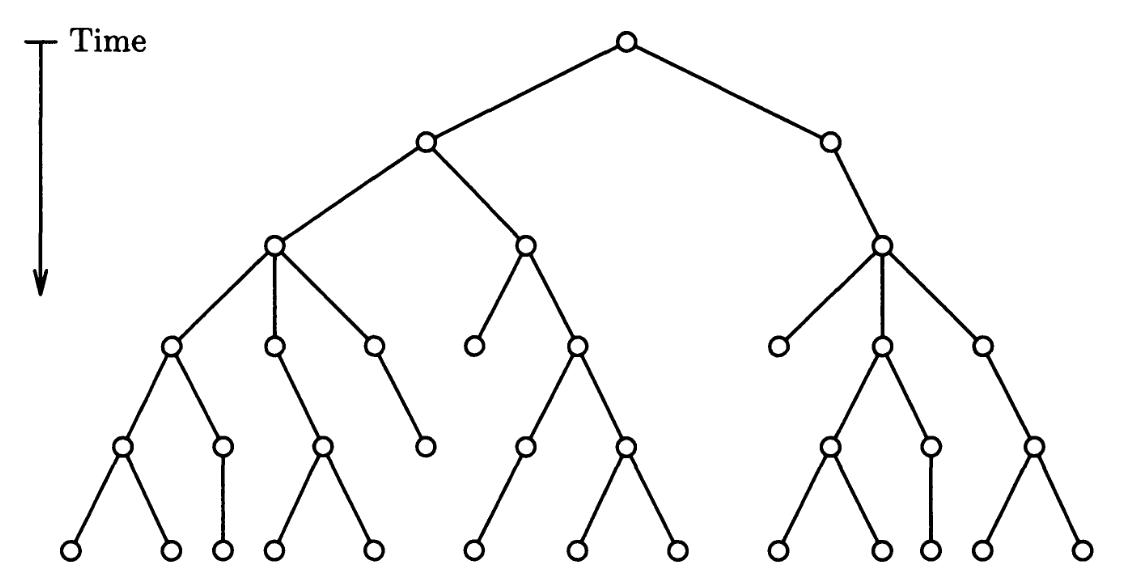
\includegraphics[width=\textwidth]{Images/Albero_configurazioni}
\end{center}
\caption{Computazione non deterministica.}\label{fig:Conf_tree}
\end{figure}

Si dice, inoltre, che una macchina di Turing non deterministica $N$ decide il linguaggio $L$ in tempo $T: \N \to \N$ sse $N$ decide $L$ e, per ogni stringa $x$ in input, ogni possibile scelta non deterministica porta a computazioni che raggiungono lo stato $q_{\mathsf{halt}}$ in un numero di passi $k \leq T(|x|)$.
Nella rappresentazione grafica $T(|x|)$ è una maggiorazione della profondità dell'albero delle possibili computazioni non deterministiche.
È interessante notare che, ad un fissato livello di profondità, il modello di macchina di Turing non deterministica esplora un insieme di possibili configurazioni esponenzialmente più grande rispetto alla macchina di Turing deterministica.

Si possono, ora, introdurre le classi di tempo non deterministico:
\begin{defn}[classe \textbf{NTIME}]\label{defn:NTIME}
 Sia $T: \N \to \N$ una funzione.
 Si definisce \textbf{NTIME}$(T)$ la classe di ogni problema decisionale $L$ per il quale esistono una costante $c > 0$ e una macchina di Turing non deterministica $N$ t.c. $N$ decide $L$ in tempo $c \cdot T$.
\end{defn}
Ovvero la trasposizione non deterministica della definizione \ref{defn:DTIME}.
In queste due definizioni, infatti, \textbf{D} indica il determinismo e \textbf{N} il non determinismo del modello computazionale utilizzato.

Si può dare, analogamente al caso di \textbf{P}, la definizione di problema risolubile in tempo polinomiale da una macchina non deterministica.
In questo caso -- come storicamente -- \textbf{NP} indica Non deterministic \textbf{P}.
\begin{defn}[classe \textbf{NP$_\mathbf{s}$}]\label{defn:NP_Ndet}
 Si definisce \textbf{NP$_\mathbf{s}$}$:= \cup_{c\geq 1}$\textbf{NTIME}$(n^c)$.
\end{defn}
Si è scelto il pedice \textbf{s} per indicare che questa è la definizione storica della classe \textbf{NP}.
Si hanno, ora, due definizioni indipendenti di \textbf{NP}, le quali risultano equivalenti:
\begin{thm}[equivalenza delle definizioni di \textbf{NP}]
 \textbf{NP$_\mathbf{s}$ = NP}
\end{thm}
\begin{proof}
 La dimostrazione si basa sul fatto che la successione di scelte che porta la macchina di Turing non deterministica a verificare l'input $x$ può essere usata come un certificato.
 \begin{enumerate}[align=left]
  \item[\textbf{NP$_\mathbf{s}$ $\subseteq$ NP:}] Sia $L \in$ \textbf{NP$_\mathbf{s}$}, allora esistono un polinomio $q: \N \to \N$ e una macchina di Turing non deterministica $N$ tali che per ogni input $x$, in un numero di passi inferiore a $q(|x|)$, $N$ giunge allo stato $q_{\mathsf{halt}}$.
  In particolare, se $x \in L$, per una particolare sequenza di scelte non deterministiche, $N$ stampa in output il valore $1$.
  Si consideri una codifica binaria della stringa che descrive le scelte.
  Se ne può individuare una tale che la lunghezza della codifica binaria sia al più $p(|x|) := c \cdot q(|x|)$ per ogni $x$, con $c \in \N$ una costante.
  
  Questa stringa opera come certificato per la definizione \ref{defn:NP_det}.
  Si può ora usare una macchina di Turing $M$ per simulare la macchina $N$, seguendo le scelte codificate dal certificato.
  Chiaramente questa simulazione può essere svolta con un solo incremento polinomiale nel tempo $q$ impiegato da $N$.
  $M$, in questo caso, verifica in tempo polinomiale che $x \in L$.
  Se, inoltre, $x \notin L$ si può prendere una qualsiasi sequenza di scelte non deterministiche e $M$ arriverà allo stato $q_{\mathsf{halt}}$, sempre in tempo polinomiale.
  La coppia $p$, $M$, dunque, soddisfa la definizione citata, per cui $L \in$ \textbf{NP}.
  
  \item[\textbf{NP$_\mathbf{s}$ $\supseteq$ NP:}] Sia $L \in$ \textbf{NP}, si considerino il polinomio $p: \N \to \N$ e la macchina di Turing $M$ come da definizione \ref{defn:NP_det}.
  Per ogni $x \in L$ esiste un certificato $u \in \left\{0,1\right\}^{p(|x|)}$ per cui $M(x,u)=1$.
  Si definisce la macchina di Turing non deterministica $N$ di $k+1$ nastri, dove $k$ è il numero di nastri di $M$, che opera nel seguente modo:
  Per le prime $p(|x|)$ operazioni scrive un carattere scelto casualmente tra $0$ e $1$ sul secondo nastro, poi opera deterministicamente.
  In particolare, nel secondo periodo, opera come la macchina di Turing $M$, considerando i primi due nastri come nastri di input (come se fossero concatenati).
  In quanto esiste un certificato $u$ di lunghezza $p(|x|)$ per cui $M(x,u)=1$, allora esiste una sequenza di scelte non deterministiche per cui $N$ stampa $u$ sul secondo nastro e arriva a stampare $1$.
  In quanto la macchina $M$ è polinomiale segue che anche $N$ lo sarà: esegue esattamente $p(|x|)$ operazioni più di quelle di $M$.
  Si è, quindi, verificato che $L \in$ \textbf{NP$_\mathbf{s}$}.\qedhere
 \end{enumerate}
\end{proof}

\subsection{Relazione tra P ed NP}
In quanto la definizione di macchina di Turing non deterministica è un'estensione di quella deterministica, risulta chiaro che ogni macchina di Turing $M$ è anche non deterministica (semplicemente non è molto interessante come tale).
È, quindi, chiaro che, per ogni funzione $T: \N \to \N$, si ha \textbf{DTIME}$(T) \subseteq$ \textbf{NTIME}$(T)$.
Da questo segue che \textbf{P} $\subseteq$ \textbf{NP}.

Purtroppo questo è il più raffinato risultato conosciuto per quanto riguarda la relazione tra \textbf{P} ed \textbf{NP}.
Uno dei $7$ problemi del millennio, infatti, chiede di stabilire se, effettivamente, \textbf{P} $\neq$ \textbf{NP}, ma rimane tutt'ora irrisolto.

Anche riprendendo i pochi esempi descritti nella sezione precedente si nota l'incompletezza delle informazioni a nostra disposizione:

\begin{enumerate}[align=left]
 \item[\textbf{Commesso viaggiatore:}] Si può dimostrare che è un problema di ``difficile'' soluzione.
 In particolare si dimostra che è in \textbf{P} sse \textbf{P} = \textbf{NP}.
 \item[\textbf{Numero composto:}] È stato recentemente mostrato, in \cite{Article:PRIMESinP}, che questo problema è in \textbf{P}.
 \item[\textbf{Fattorizzazione:}] Tutt'ora non si sa se sia, o meno, in \textbf{P} o se sia ``difficile'' quanto il problema del commmesso viaggiatore.
 Si suppone, assumendo \textbf{P} $\neq$ \textbf{NP}, che sia in \textbf{NP}$\setminus$\textbf{P}.
 È per questa ragione che esistono sistemi crittografici basati sul problema della fattorizzazione degli interi.
\end{enumerate}

\section{Classi di complessità quantistica}
Per ora è stata introdotta la sola teoria classica.
Per passare allo studio degli algoritmi che seguiranno è necessario formalizzare il modello dei circuiti, in particolare quantistici, e introdurre le definizioni, che riprendano quelle date nelle sezioni precedenti, per richieste computazionali e classi di complessità.

\subsection{Circuiti Booleani e complessità}
Nel primo capitolo si è data una nozione informale e operativa di circuito, per comprendere il funzionamento di un computer quantistico.
Segue una definizione più formale dei circuiti classici utilizzati per computare funzioni di Boole, associate ai problemi decisionali.
\begin{defn}[Circuito booleano]
 Si definisce {\upshape circuito booleano} con $n$ bit di input un grafo aciclico diretto nel quale i nodi possono essere:
 \begin{itemize}
  \item {\upshape nodi di input}, di grado entrante $0$, etichettati da uno degli $n$ bit dell'input,
  \item {\upshape porte logiche}, con grado entrante $1$ o $2$, scelte tra i gate \textsc{and}, \textsc{or} e \textsc{not}.
 \end{itemize}
 Tra questi nodi si sceglie un gate logico come porta di {\upshape output} del circuito.
\end{defn}
Ogni nodo con grado entrante maggiore di 1 è detto gate logico o porta logica.
Si indica con $C(x)$ l'output del circuito $C$ a partire dall'input $x$.
Si definiscono, inoltre, \textit{dimensione} del circuito il numero di porte logiche che possiede e \textit{profondità} del circuito la massima lunghezza di un cammino da una porta di input alla porta di output.

Risulta chiaro che, ogni circuito booleano con $n$ bit di input, computa una funzione booleana $f:\{0,1\}^n \to \{0,1\}$.
Si può, quindi, pensare di utilizzare dei circuiti per decidere linguaggi, o problemi decisionali.
In generale, però, un linguaggio -- o la sua codifica binaria -- contiene elementi di diversa lunghezza, per cui non basta un singolo circuito per decidere un intero linguaggio.
Si deve, infatti, introdurre la nozione di \textit{famiglia di circuiti}. 
Essa è una successione $\left\{ C_n \right\}_{n \in \N}$ di circuiti booleani, in cui il circuito $C_n$ opera su input di lunghezza binaria $n$.

Dato un linguaggio $L$, quindi, esiste sempre una famiglia di circuiti $\left\{ C_n \right\}_{n \in \N}$ che decide il linguaggio $L$, ovvero che ne computa la funzione booleana associata.
Si dice che questa famiglia è di \textit{dimensione minimale} (rispettivamente di \textit{profondità minimale}) se non esistono famiglie, che decidono lo stesso linguaggio, di dimensione (rispettivamente profondità) minore.

A partire da questi concetti, quindi, si dà la seguente definizione:
\begin{defn}[Complessità della dimensione dei circuiti]
 Dato un linguaggio formale $L$ si definisce {\upshape complessità della dimensione} dei circuiti la funzione $T: \N \to \N$, che associa ad ogni $n$ la dimensione di $C_n$, ovvero dell'$n$-esimo circuito della famiglia di dimensione minimale che decide $L$.
\end{defn}
Sostituendo profondità a dimensione si ottiene l'analoga definizione per la \textit{complessità di profondità} dei circuiti.

Il fatto che input di lunghezza diversa siano analizzati da circuiti distinti rende questo modello di computazione non uniforme.
A priori, infatti, in una famiglia di circuiti, non è richiesta alcuna relazione tra i vari elementi della famiglia.
Per studiare le classi di complessità originate da questo modello computazionale si introduce il concetto di uniformità.
Intuitivamente una famiglia è uniforme se esiste un algoritmo che descriva, in funzione della sola dimensione $n$ dell'input, come costruire il corrispondente circuito $C_n$.
Inoltre si distinguono vari tipi di uniformità in funzione delle risorse impiegate dall'algoritmo richiesto.

In particolare saranno utili le seguenti famiglie uniformi di circuiti (non solo booleani):
\begin{defn}[Famiglia uniforme in tempo polinomiale]\label{defn:Unif_family}
 Una famiglia di circuiti $\left\{ C_n \right\}_{n \in \N}$ si dice {\upshape uniforme in tempo polinomiale} sse esiste una macchina di Turing deterministica $M$ tale che:
 \begin{itemize}
  \item $M$ opera in tempo polinomiale,
  \item per ogni $n \in \N$ la macchina $M$ produce una descrizione del circuito $C_n$ sull'input della stringa contenente esattamente $n$ simboli $1$, denotata con $1^n$.
 \end{itemize}
\end{defn}

\subsection{Circuiti quantistici}\label{sec:QCircuits}
In analogia ai circuiti booleani si definiscono i circuiti quantistici:
\begin{defn}[Circuito quantistico]
 Si definisce {\upshape circuito quantistico} con $n$ qubit di input un grafo aciclico diretto nel quale i nodi possono essere:
 \begin{itemize}
  \item {\upshape nodi di input}, di grado entrante $0$, etichettati da uno degli $n$ qubit dell'input,
  \item {\upshape porte logiche}, con grado entrante uguale a quello uscente, scelte in una fissata famiglia di gate.
%  \item misure nella base computazionale, con grado uscente pari a quello entrante.
 \end{itemize}
 Di questi nodi si scelgono $m$ nodi con grado entrante maggiore di zero, ai quali si associa l'{\upshape output} del circuito.
\end{defn}
Dai nodi di output si vuole ottenere dell'informazione classica.
%Se il nodo scelto è una misura non si deve operare ulteriormente, altrimenti è necessario far seguire la porta logica da un'opportuna misura nella base computazionale.
È necessario, quindi, far seguire la porta logica di output da un'opportuna misura nella base computazionale, nell'implementazione del circuito.
Per un circuito $QC$ si indica l'output con $QC(x)$, dove $x$ è lo stato quantistico di input.
La famiglia di gate tra cui scegliere le porte logiche potrebbe essere finita o infinita.
Nella realizzazione fisica si è più portati a scegliere famiglie finite di porte logiche, per ovvie questioni pratiche.
A tal fine è importante lo studio di quelle che sono chiamate famiglie di gate universali, svolto in \cite{Book:QCQI}.
A differenza dei gate universali classici, che possono computare ogni funzione a valori in stringhe binarie, le famiglie universali quantistiche possono \textit{approssimare}, con arbitraria precisione, qualsiasi gate realizzabile.

Per scopi più teorici, invece, è utile considerare la famiglia infinita contenente tutti i gate su un singolo qubit e il gate \textsc{cnot}.
Essa, infatti, si dimostra essere sufficiente a simulare il comportamento di qualsiasi altro gate quantistico.
Per approfondire questo argomento si rimanda a \cite{Book:QCQI}.

\subsubsection{Classi di complessità}
Su questo modello computazionale si ripropongono, senza alterazioni, le nozioni di complessità della dimensione e della profondità dei circuiti.
Si riporta, per chiarezza, la prima:
\begin{defn}[Complessità della dimensione dei circuiti]
 Dato un linguaggio formale $L$ si definisce {\upshape complessità della dimensione} dei circuiti la funzione $T: \N \to \N$, che associa ad ogni $n$ la dimensione di $QC_n$, ovvero dell'$n$-esimo circuito della famiglia di dimensione minimale che decide $L$.
\end{defn}
Questa stima sarà spesso utilizzata nel capitolo seguente, per analizzare l'efficienza degli algoritmi sviluppati.
In particolare si userà la notazione asintotica descritta nella definizione \ref{defn:Oh_notation}.
Si dirà, dunque, che un algoritmo ha un costo computazionale di $O(T)$ gate per affermare che la corrispondente famiglia di circuiti ha complessità di dimensione $F = O(T)$.

Come per la complessità, anche i concetti di famiglia uniforme e, in particolare, di famiglia uniforme in tempo polinomiale, definizione \ref{defn:Unif_family}, si traspongono senza alterazione alcuna.

Si possono, ora, definire le classi di complessità quantistiche equivalenti a \textbf{P} ed \textbf{NP}.
La differenza principale con le precedenti, a meno del differente modello computazionale, risiede nella natura aleatoria della computazione quantistica. Si sarà, infatti, costretti a richiedere una minima probabilità di successo degli algoritmi.
\begin{defn}[classe BQP]\label{defn:BQP}
 La classe \textbf{BQP} contiene tutti i problemi decisionali $L$ che ammettono una famiglia uniforme in tempo polinomiale di circuiti quantistici $\left\{ QC_n \right\}_{n \in \N}$ tale che:
 \begin{itemize}
  \item Per ogni $n$ il circuito $QC_n$ prende in input $n$ qubit e restituisce in output un singolo bit,
  \item Per ogni $x \in L$ vale $\P\left(QC_{|x|}(x) = 1\right) \geq 2/3$
  \item Per ogni $x \notin L$ vale $\P\left(QC_{|x|}(x) = 0\right) \geq 2/3$
 \end{itemize}
\end{defn}
La sigla \textbf{BQP} rappresenta: ``Bounded-error Quantum Polynomial time''.
Si richiede, infatti, l'esistenza di una famiglia di circuiti, di cui si può ottenere una descrizione in tempo polinomiale tramite una macchina di Turing e che ha una probabilità di errore limitata.
Si noti che il valore $2/3$ è, fondamentalmente, simbolico.
La ripetizione, di un algoritmo che rispetti tale condizione, un numero costante di volte diminuisce esponenzialmente la probabilità di errore -- ogni ripetizione è indipendente -- rispettando comunque le condizioni della definizione.

Analogamente alla classe \textbf{P} si considerano i problemi in \textbf{BQP} come efficientemente risolubili da una computer quantistico.
Tutti gli algoritmi che verranno studiati nel prossimo capitolo soddisfano le condizioni appena esposte, ovvero risolvono problemi in questa classe di complessità.
Intuitivamente ciò è dovuto al fatto che si riesce a dare una descrizione esplicita dei circuiti che li implementano, indipendentemente dalla lunghezza degli input, in questa breve trattazione.

Mentre, come è reso evidente dai risultati trovati da Fredkin e Toffoli è noto che \textbf{P} $\subseteq$ \textbf{BQP}, attualmente non è conosciuta alcuna relazione tra le classi \textbf{NP} e \textbf{BQP}.
Ci sono, però, evidenze che \textbf{NP} $\nsubseteq$ \textbf{BQP}.
Inoltre, per quanto un computer quantistico possa essere fondamentalmente più veloce di un computer classico, è stato dimostrato che non sarà esponenzialmente più veloce di esso.

Si passa, ora, all'analogo quantistico di \textbf{NP}:
\begin{defn}[classe QMA]\label{defn:QMA}
 Si definisce \textbf{QMA} la classe contenente tutti i linguaggi $L \subseteq \left\{0,1\right\}^*$ tali per cui esistono un polinomio $p: \N \to \N$ e una famiglia uniforme in tempo polinomiale di circuiti quantistici $\left\{ QC_n \right\}_{n \in \N}$ tali che:
 \begin{align}
  \forall\, x \in L\ \exists \ket{\psi} \in \left(\C{2}\right)^{\otimes p(|x|)} \text{ t.c. }& \P\left( QC_{|x|}(\ket{x},\ket{u}) = 1 \right) \geq \frac{2}{3}\\
  \forall\, x \notin L\ , \forall\, \ket{\psi} \in \left(\C{2}\right)^{\otimes p(|x|)} \text{ si ha }& \P\left( QC_{|x|}(\ket{x},\ket{u}) = 1 \right) \leq \frac{1}{3}
 \end{align}
\end{defn}
Tale definizione riprende la definizione deterministica di problemi per i quali esiste un certificato efficientemente verificabile.
Come nel caso di \textbf{BQP} le differenze principali dalla definizione classica sono le seguenti.
Innanzitutto si ammette una probabilità di errore per la natura probabilistica della computazione quantistica.
Inoltre si richiede che il certificato sia di natura quantistica, ovvero un $p(|x|)$-qubit.

\chapter{Algoritmi quantistici}\label{chap:algorithms}
Con gli strumenti sviluppati fin'ora si possono, finalmente, studiare i primi algoritmi quantistici.
Innanzitutto verranno presentati degli algoritmi che sfruttano il comportamento quantistico del modello computazionale esibendo comportamenti impossibili in quello classico.
In seguito verranno trattati degli algoritmi per la risoluzione di importanti problemi dal punto di vista pratico.
Tali algoritmi si baseranno sulla \textit{trasformata di Fourier quantistica}, una riscrittura in termini quantistici della \textit{trasformata di Fourier discreta}, alla base di molti algoritmi efficienti in termini classici.
È notevole osservare che tutti questi algoritmi mostreranno richieste computazionali decisamente minori, a volte anche in modo esponenziale, rispetto alle migliori controparti classiche.

\section{Fenomeni quantistici}\label{sec:Quantum_phenomena}
Come introdotto nella sezione \ref{sec:paragone_cc} il modello di computazione quantistica gode di svariate peculiarità rispetto alla computazione classica.
La sezione citata si concentra sulle mancanze della prima rispetto all'ultima, in questa, invece, si mostreranno alcuni fenomeni che non sono replicabili classicamente.
In particolare si tratteranno alcuni possibili vantaggi ottenibili con il nuovo paradigma di computazione.

\subsection{Stati di Bell}\label{sec:Bell_states}
\begin{figure}[h]
 \begin{center}
  \bgroup
   %Il bgroup è per avere un minimo di padding verticale nella tabella
   \def\arraystretch{1.3}
   \begin{tabular}{ l | c }
       \hline
       In & Out  \\ \hline
       $\ket{00}$ & $\left( \ket{00} + \ket{11} \right)/\sqrt{2} =: \ket{\beta_{00}}$  \\
       $\ket{01}$ & $\left( \ket{01} + \ket{10} \right)/\sqrt{2} =: \ket{\beta_{01}}$  \\
       $\ket{10}$ & $\left( \ket{00} - \ket{11} \right)/\sqrt{2} =: \ket{\beta_{10}}$  \\
       $\ket{11}$ & $\left( \ket{01} - \ket{10} \right)/\sqrt{2} =: \ket{\beta_{11}}$  \\
       \hline
   \end{tabular}
  \egroup
  \quad \quad
  \begin{quantikz}[column sep=1.8em, row sep=2.2em, thin lines]
   \lstick{$\ket{x}$} & \gate{H} & \ctrl{1} & \qw\rstick[wires=2]{$\ket{\beta_{xy}}$} \\
   \lstick{$\ket{y}$} & \qw & \targ{} & \rstick{} \qw
  \end{quantikz}
 \end{center}
 \caption{Circuito che costruisce gli stati di Bell a partire dagli elementi della base computazionale. Nella tabella sono elencati gli output del circuito, al variare dei valori in input.}\label{fig:Bell_states}
\end{figure}
A partire dagli elementi della base computazionale il circuito rappresentato in figura \ref{fig:Bell_states} produce i seguenti stati:
\begin{align}
 \ket{\beta_{00}} &= \frac{\ket{00} + \ket{11}}{\sqrt{2}}\\
 \ket{\beta_{01}} &= \frac{\ket{01} + \ket{10}}{\sqrt{2}}\\
 \ket{\beta_{10}} &= \frac{\ket{00} - \ket{11}}{\sqrt{2}}\\
 \ket{\beta_{11}} &= \frac{\ket{01} - \ket{10}}{\sqrt{2}}
\end{align}
in cui la notazione $\ket{\beta_{xy}}$, oltre a rappresentare gli stati di partenza su cui opera il circuito \ref{fig:Bell_states}, può essere usata per ottenere l'esplicita espressione del corrispondente stato di Bell tramire la seguente espressione
\begin{align}
 \ket{\beta_{xy}} = \frac{\ket{0y} + (-1)^x \ket{1\bar{y}}}{\sqrt{2}},
\end{align}
dove $\bar{y} := \neg y$ è la negazione di $y$.

Questi stati sono noti con il nome di \textit{stati di Bell} o \textit{stati EPR} in onore di Bell, Einstein, Podolsky e Rosen, i quali per primi hanno studiato le proprietà di questi speciali stati.
Essi, infatti, sono stati entangled, come è stato mostrato per $\ket{\beta_{00}}$ nella sezione \ref{sec:entanglement}, e formano una base per $\C{4}$.
Quest'ultima affermazione, in particolare, è evidente dal fatto che sono immagini tramite un circuito quantistico, ovvero un operatore unitario, degli elementi della base computazionale.

Questi stati, inoltre, sono legati dalle seguenti relazioni, che implicitamente giocheranno un ruolo molto importante nelle prossime sezioni:
\begin{align}\label{eqn:Bell_identities}
 Id \otimes Id \ket{\beta_{00}} = Id \otimes Id \ket{\beta_{00}} = \ket{\beta_{00}};&\
 X \otimes Id \ket{\beta_{00}} = Id \otimes X \ket{\beta_{00}} = \ket{\beta_{01}};\\
 Z \otimes Id \ket{\beta_{00}} = Id \otimes Z \ket{\beta_{00}} = \ket{\beta_{10}};&\
 iY \otimes Id \ket{\beta_{00}} = Id \otimes iY \ket{\beta_{00}} = \ket{\beta_{11}}
\end{align}
dove $Id, X, Y$ e $Z$ sono le matrici di Pauli, per cui
\begin{align}
 Id  = 
 \begin{bmatrix}
  1 & 0\\
  0 & 1
 \end{bmatrix};\ \
 X  = 
 \begin{bmatrix}
  0 & 1\\
  1 & 0
 \end{bmatrix};\ \
 Z = 
 \begin{bmatrix}
  1 & 0\\
  0 & -1
 \end{bmatrix};\ \
 iY = ZX = 
 \begin{bmatrix}
  0 & 1\\
  -1 & 0
 \end{bmatrix}.
\end{align}


\subsection{Teletrasporto quantistico}\label{sec:QTeleportation}
Si sfrutteranno, ora, le peculiarità degli stati di Bell per ottenere un risultato sorprendente e di grande utilità per la comprensione del funzionamento dei computer quantistici. 
L'obiettivo del seguente algoritmo, detto di \textit{teletrasporto quantistico}, è di trasmettere lo stato $\ket{\psi}$ di un qubit tra due computer quantistici, rispettivamente in mano ad Alice e Bob, scambiando solamente 2 bit di informazione classica.
Senza un precedente scambio di informazioni tale processo è chiaramente impossibile, in quanto, come evidenziato nelle sezioni precedenti, lo stato di un qubit è descritto da 3 valori reali, che richiederebbero una quantità infinita di bit classici per essere descritti. 

\begin{figure}
 \begin{center}
  \begin{quantikz}[column sep=2em, row sep=1.6em, thin lines, slice style=black]
   \lstick{$\ket{\psi}$} & \qw \slice{$\ket{\psi_0}$} & \ctrl{1} \slice{$\ket{\psi_1}$} & \gate{H} \slice{$\ket{\psi_2}$} & \meter{} \rstick{$\ M_1$\\\vspace{1.5mm}} & \cw \slice{$\ket{\psi_3}$} & \cw  & \cwbend{2} \slice{$\ket{\psi_4}$} & \\
   \lstick[wires=2]{$\ket{\beta_{00}}$} & \qw & \targ{} & \qw & \meter{} \rstick{$\ M_2$\\\vspace{1.5mm}} & \cw  & \cwbend{1} & \\
   & \qw & \qw & \qw & \qw & \qw & \gate{X^{M_2}} & \gate{Z^{M_1}} & \rstick{$\ket{\psi}$}\qw 
  \end{quantikz}
 \end{center}
 \caption{Circuito per l'algoritmo di teletrasporto quantistico. Lo stato $\ket{\psi}$ passa dal primo all'ultimo registro, tramite sola comunicazione classica.}\label{crq:Quantum_teleportation}
\end{figure}

Per sorvolare questo problema si crea uno stato entangled di Bell, per semplicità $\ket{\beta_{00}}$, e si dà il primo qubit di questa coppia ad Alice e il secondo a Bob.
Per quanto i due computer quantistici possano essere separati da una grande distanza spaziale, si descriverà il sistema con un unico stato dei 3-qubit, in cui, inizialmente, il primo (da trasmettere) sarà nello stato $\ket{\psi} = a \ket{0} + b \ket{1}$ e gli altri due in quello entangled $\ket{\beta_{00}}$.
Di questo stato i valori $a$ e $b$ sono arbitrari e, a priori, sconosciuti.
Si assume, inoltre, che i primi due qubit siano in possesso di Alice e solo il terzo di Bob.
Lo stato iniziale, quindi, sarà
\begin{equation}
 \ket{\psi_0} := \ket{\psi}\ket{\beta_{00}} = \frac{1}{\sqrt{2}}\left\{ a\ket{0} \left(\ket{00} + \ket{11} \right) + b\ket{1} \left(\ket{00} + \ket{11} \right) \right\},
\end{equation}
come indicato in figura \ref{crq:Quantum_teleportation}. Inizialmente Alice agisce sulla propria coppia di qubit, prima con un gate \textsc{cnot}, ad ottenere lo stato
\begin{equation}
 \ket{\psi_1} = \frac{1}{\sqrt{2}}\left\{a \ket{0} \left(\ket{00} + \ket{11} \right) + b \ket{1} \left(\ket{10} + \ket{01} \right) \right\}
\end{equation}
e, poi, con un gate Hadamard sul primo qubit, ad ottenere
\begin{equation}
 \ket{\psi_2} = \frac{1}{2} \left\{a \left(\ket{0} + \ket{1} \right) \left(\ket{00} + \ket{11} \right) + b \left(\ket{0} - \ket{1} \right) \left(\ket{10} + \ket{01} \right) \right\}.
\end{equation}
Questo stato, in particolare, può essere riscritto raggruppando i primi 2 qubit, in possesso di Alice, come segue
\begin{align}
 \ket{\psi_2} = \frac{1}{2}\{&\ket{00} \left(a\ket{0} + b\ket{1} \right) + \ket{01} \left(a\ket{1} + b\ket{0} \right) \nonumber \\
 + &\ket{10} \left(a\ket{0} - b\ket{1} \right) + \ket{11} \left(a\ket{1} - b\ket{0} \right) \}.
\end{align}
In questo stato, Alice, misurando la propria coppia di qubit, forzerà, a causa dell'entanglement della coppia di Bell, il bit di Bob ad assumere uno dei $4$ stati appena elencati. 
In particolare, in funzione della misurazione $M_1M_2$ di Alice, lo stato del qubit di Bob sarà $\ket{\psi_3(M_1M_2)}$, più esplicitamente:
\begin{align}\label{eqn:QT_post_measure1}
 M_1M_2 = 00 \implies \ket{\psi_3(00)} &= \left( a \ket{0} + b \ket{1} \right)\\
 M_1M_2 = 01 \implies \ket{\psi_3(01)} &= \left( a \ket{1} + b \ket{0} \right)\\
 M_1M_2 = 10 \implies \ket{\psi_3(10)} &= \left( a \ket{0} - b \ket{1} \right)\\
 M_1M_2 = 11 \implies \ket{\psi_3(11)} &= \left( a \ket{1} - b \ket{0} \right).\label{eqn:QT_post_measure4}
\end{align}
A questo punto, in seguito alla comunicazione della coppia di bit dalla misurazione di Alice dei propri qubit, Bob può provvedere ad operare sul qubit in suo possesso per ottenere $\ket{\psi}$.
In particolare dovrà agire con le seguenti operazioni:
\begin{align}
 M_1M_2 = 00 \implies Id\ket{\psi_3(00)} =& \left( a \ket{0} + b \ket{1} \right) = \ket{\psi}\\
 M_1M_2 = 01 \implies X\ket{\psi_3(01)} =& \left( a \ket{0} + b \ket{1} \right) = \ket{\psi}\\
 M_1M_2 = 10 \implies Z\ket{\psi_3(10)} =& \left( a \ket{0} + b \ket{1} \right) = \ket{\psi}\\
 M_1M_2 = 11 \implies ZX\ket{\psi_3(11)} =& \left( a \ket{0} + b \ket{1} \right) = \ket{\psi}.
\end{align}
In particolare, nell'ultima riga si opera con la trasformazione $ZX$, che corrisponde ad applicare prima il gate $X$ e poi il gate $Z$, come rappresentato nel circuito \ref{crq:Quantum_teleportation}, in cui le operazioni si susseguono da sinistra a destra.
Inoltre risulta chiaro dal prospetto precedente che le operazioni corrette per ottenere lo stato $\ket{\psi}$, data la misurazione $M_1M_2$, sono $Z^{M_1}X^{M_2}$, ovvero quanto rappresentato nel circuito, in cui lo stato finale, correttamente, è proprio $\ket{\psi}$.

Questo interessante fenomeno merita due ulteriori commenti prima di essere abbandonato.
Innanzitutto potrebbe parre che, trasportando lo stato del qubit $\ket{\psi}$ da Alice a Bob, se ne stia creando una copia, in violazione del teorema \ref{thm:N-C} (no cloning theorem).
Ciò non è vero, in quanto, in seguito alla misurazione della coppia di qubit di Alice, il primo registro, in cui era immagazzinato lo stato $\ket{\psi}$, si ritrova in uno dei due stati della base computazionale: $\ket{0}$ o $\ket{1}$.
Si ottiene, quindi, una sola copia dello stato $\ket{\psi}$, senza alcuna contraddizione del suddetto teorema.

Un'ulteriore commento, di natura più fisica, riguarda la parvenza che questo circuito permetta, in contraddizione con la teoria della relatività generale, la trasmissione di informazione a velocità superluminale.
Questa idea potrebbe essere scatenata dal fatto che la misurazione dei qubit di Alice porta all'immediato ``collasso'' del qubit di Bob a uno degli stati in \eqref{eqn:QT_post_measure1}-\eqref{eqn:QT_post_measure4}. 
Anche questa affermazione è solo apparentemente vera: per ottenere lo stato del primo qubit Bob deve attendere l'informazione classica della misurazione effettuata da Alice, la quale non può essere trasmessa a velocità superluminali.
In realtà, con strumenti matematici più potenti rispetto a quelli introdotti in questa breve trattazione, si può mostrare che, senza lo scambio dei bit classici, il solo fenomeno di entaglement non trasferisce alcuna informazione -- si veda \cite{Book:QCQI} alla sezione 2.4.3.

\subsection{Superdense coding}
\begin{figure}[h]
 \begin{center}
  \begin{quantikz}[column sep=1.5em, row sep=1.6em, thin lines,slice style=black]
   \lstick{$\ket{0}$} & \gate{H}\gategroup[2,steps=2,style={dashed, inner xsep=2pt}, background, label style={label position=below,anchor=north,yshift=-0.2cm}]{Preparazione} & \ctrl{1} & \qw \slice{$\ket{\beta_{00}}$} & \qw & \gate{X^{b_2}}\gategroup[1,steps=2,style={dashed, inner xsep=2pt}, background, label style={label position=above,anchor=south,yshift=-0.2cm}]{Alice} & \gate{Z^{b_1}} & \qw\slice{$\ket{\beta_{b_1b_2}}$} & \qw & \ctrl{1}\gategroup[2,steps=5,style={dashed, inner xsep=2pt}, background, label style={label position=below,anchor=north,yshift=-0.2cm}]{Bob} & \gate{H}\slice{$\ket{b_1b_2}$} & \meter{} & \cw \rstick{$b_1$} & \\
   \lstick{$\ket{0}$} & \qw & \targ{} & \qw & \qw &\qw\gategroup[1,steps=4,style={dashed, inner xsep=2pt}, background, label style={label position=below,anchor=north,yshift=-0.2cm}]{Bob} & \qw & \qw & \qw & \targ{} & \qw & \meter{}  & \cw \rstick{$b_2$} &
  \end{quantikz}
 \end{center}
 \caption{Circuito per l'algoritmo di superdense coding. Permette la trasmissione di 2 bit classici tramite lo scambio di 1 solo qubit.}\label{crq:Superdense_coding}
\end{figure}

L'algoritmo precedente ha una controparte, che sfrutta sempre gli stati entangled di Bell, per ottenere l'effetto opposto: inviare due bit classici $b_1$ e $b_2$, tramite lo scambio di un singolo qubit da Alice a Bob.
Tale algoritmo è chiamato \textit{superdense coding} ed è rappresentato nel circuito in figura \ref{crq:Superdense_coding}.
Per comprenderne appieno il funzionamento si commentano i vari stadi del circuito.
Nel riquadro ``Preparazione'', a partire da $\ket{00}$, viene preparato lo stato $\ket{\beta_{00}}$, come descritto in sezione \ref{sec:Bell_states}.
Il primo qubit di questo stato viene dato ad Alice, mentre il secondo a Bob.
Come descritto dalle identità in \eqref{eqn:Bell_identities} Alice trasforma il qubit $\ket{\beta_{00}}$ in $\ket{\beta_{b_1b_2}}$, dove $b_1$ e $b_2$ sono i bit classici che vuole trasmettere a Bob.
A questo punto Alice invia anche il proprio qubit a Bob, il quale è, ora, in possesso di entrambi i componenti dello stato entangled.
Per reversibilità degli operatori quantistici Bob, eseguendo al contrario il circuito quantistico in figura \ref{fig:Bell_states} ottiene, a partire da $\ket{\beta_{b_1b_2}}$, lo stato della base computazionale $\ket{b_1b_2}$.
A Bob non resta che misurare lo stato in proprio possesso nella base computazionale per ottenere, con certezza, la coppia di bit $b_1b_2$ che Alice doveva comunicargli, come ci si era prefissati.

Gli ultimi due algoritmi mostrano come, fondamentalmente, la capacità di memoria di un sistema di $n$-qubit sia $2^n$ bit classici, dando alla computazione quantistica, su questo fronte, un vantaggio esponenziale rispetto a quella classica.

\subsection{Parallelismo quantistico}\label{sec:Quantum_par}
Una fondamentale caratteristica dei computer quantistici è la possibilità di valutare svariati valori di una funzione binaria contemporaneamente. Questa proprietà è chiamata \textit{parallelismo quantistico} ed è alla base di tutta la sezione \ref{sec:QFT}, in cui la trasformata di Fourier quantistica ne farà uso.

Per comprendere appieno le potenzialità, ma soprattutto le limitazioni, di questo peculiare comportamento quantistico è necessario osservarne il funzionamento nel dettaglio.
Per chiarezza sarà trattato per primo il caso di una funzione $f:\left\{ 0,1 \right\} \to \left\{ 0,1 \right\}$ arbitraria.
Questa funzione non è necessariamente unitaria (o invertibile), quindi non è immediatamente implementabile quantisticamente.
Si può, però, decidere di tenere in memoria sia il valore in entrata alla funzione, sia l'immagine della funzione.
Si crea, quindi, il gate $U_f$ che manda il generico stato $\ket{x,y}$ in $\ket{x,y \oplus f(x)}$, dove $\oplus$ indica la somma modulo 2. Per funzioni binarie come $f$, inoltre, tale trasformazione è unitaria.

In particolare, se $y=0$, lo stato $\ket{x,0}$ verrà mandato da $U_f$ in $\ket{x, f(x)}$, dando esplicitamente il valore della funzione. La parte interessante del procedimento per ottenere il parallelismo quantistico, però, si incontra analizzando $x$.
Infatti, ponendo $\ket{x} = \left(\ket{0} + \ket{1} \right)/\sqrt{2}$ -- facilmente preparabile applicando un gate $H$ a un qbit nello stato $\ket{0}$ -- $U_f$ agirà nel seguente modo:
\begin{equation}
 \ket{x,0} = \frac{\ket{0} + \ket{1}}{\sqrt{2}}\ket{0} \stackrel{U_f}{\longmapsto} \frac{\ket{0,f(0)} + \ket{1,f(1)}}{\sqrt{2}}.
\end{equation}
In questo stato sono presenti entrambe le immagini della funzione $f$ e queste sono state computate simultaneamente, da un singolo circuito.

Analogamente, data una funzione $f:\left\{ 0,1 \right\}^n \to \left\{ 0,1 \right\}^m$, si definisce un gate $U_f$, che opera come
\begin{equation}
 \ket{x,y} \stackrel{U_f}{\longmapsto} \ket{x,y + f(x) \mod 2^m}.
\end{equation}
Scrivendone la rappresentazione come matrice risulta chiaro che è anch'esso unitario. 
Si può persino mostrare che, se esiste un algoritmo classico per computare $f:\left\{ 0,1 \right\}^n \to \left\{ 0,1 \right\}^m$, allora l'algoritmo quantistico per computare $U_f$ è di paragonabile efficienza.
Per approfondire si rimanda a \cite{Book:QCQI}, sezione 3.2.5.\\
In particolare, a partire dallo stato 
\begin{equation}
 \ket{x}\ket{y} := \left(\frac{1}{2^{n/2}}\sum_{j=0}^{2^n-1} \ket{j}\right)\ket{0} = 
 \frac{1}{2^{n/2}}\sum_{j=0}^{2^n-1} \ket{j}\ket{0},
\end{equation}
il gate $U_f$ produrrà lo stato
\begin{equation}
 \frac{1}{2^{n/2}}\sum_{j=0}^{2^n-1} \ket{j}\ket{f(j)},
\end{equation}
il quale, come nel caso precedente, contiene tutte le immagini di $f$.
In particolare lo stato $\ket{x}$ iniziale può essere facilmente preparato applicando un gate Hadamard $H^{\otimes n}$ allo stato $\ket{0}{\otimes n}$.

A seguito di quest'analisi risulta chiaro che il circuito quantistico alla base del parallelismo quantistico corrisponda con quanto rappresentato in figura \ref{crq:Quantum_parallelism}.
Inoltre, per lo scopo attuale, non è importante conoscere la realizzazione del gate $U_f$, ma solo il fatto che possa essere realizzato.
Per l'applicabilità del processo di parallelismo può essere semplicemente considerato come una scatola nera.

\begin{figure}[h]
 \begin{center}
  \begin{quantikz}[column sep=2em, row sep=1.6em, thin lines]
   \lstick{$\ket{0}$} & \gate{H^{\otimes n}}\qwbundle{n} & \gate[wires=2][2cm]{U_f}\gateinput{$x$}\gateoutput{$x$} & \qw\rstick[wires=2]{$\displaystyle{\frac{1}{2^{n/2}}\sum_{x=0}^{2^n-1}\ket{x}\ket{f(x)}}$}\\
   \lstick{$\ket{0}$} & \qw\qwbundle{m} & \gateinput{$y$}\gateoutput{$y \oplus f(x)$} & \qw
  \end{quantikz}
 \end{center}
 \caption{Circuito per l'algoritmo di parallelismo quantistico. Crea uno stato finale contenente la valutazione della funzione $f$ su tutti gli elementi del proprio dominio.}
 \label{crq:Quantum_parallelism}
\end{figure}

Ora che è chiaro il funzionamento dell'algoritmo si possono analizzare più nel dettaglio le sue proprietà.
Innanzitutto, indipendentemente dalla grandezza del dominio della funzione $f$, supposto di aver abbastanza memoria per poter rappresentare tutti gli elementi del dominio, basta un singolo circuito quantistico per operare con il parallelismo. 
In ambito classico, per valutare la funzione su tutti gli elementi del dominio in contemporanea sarebbe necessario un circuito per ciascun elemento, con una richiesta di risorse fisiche esponenzialmente più grande.

Nonostante questo grandissimo vantaggio, purtroppo, lo stato finale di questo circuito non è immediatamente accessibile: per osservarlo sarebbe necessario misurarlo, facendolo collassare su un solo elemento della sovrapposizione.
Ciò restituirebbe come risultato l'immagine di un singolo elemento del dominio, scelto casualmente, cancellando il resto della computazione.
Questo fatto comporta la necessità di sfruttare in modo meno diretto la grande quantità di informazioni contenuta nella sovrapposizione.
È necessario, infatti, in base al problema da affrontare, operare ulteriormente sullo stato preparato dal parallelismo, per ottenere, con grande probabilità, un risultato corretto.
Per mostrare come ciò possa essere messo in atto, nella prossima sezione, verrà analizzato un problema la cui risoluzione quantistica si basa su un ingegnoso uso del parallelismo.

\subsection{Algoritmo di Deutsch-Josza}\label{sec:Deutsch-Josza}
L'algoritmo di \textit{Deutsch-Josza} si pone un problema di poca utilità pratica, ma grande utilità didattica.
Servirà per comprendere come il parallelismo quantistico possa essere utilizzato per risolvere problemi in cui è necessario valutare una funzione più volte.
Innanzitutto è necessario spiegare il problema da risolvere.
Sia $f:\left\{0,1\right\}^n \to \left\{0,1\right\}$ una funzione binaria.
Tale funzione deve, inoltre, essere \textit{costante}, ovvero assumere lo stesso valore per ogni elemento del dominio, oppure \textit{bilanciata}, ovvero asssumere il valore $1$ esattamente la metà delle volte e $0$ l'altra metà.
L'algoritmo di \textit{Deutsch-Josza}, con una sola esecuzione della scatola nera $U_f$ vuole individuare con certezza se la corrispondente funzione $f$ è bilanciata o costante.
Per ottenere tale risultato si opera, come descritto nel circuito della figura \ref{crq:Deutsch-Josza}, applicando un circuito di \textit{parallelismo quantistico} e manipolando lo stato ottenuto in modo tale da far interferire tra loro gli elementi della sovrapposizione, fino a poter misurare, con certezza, una risposta al problema.

\begin{figure}[h]
 \begin{center}
  \begin{quantikz}[column sep=2em, row sep=1.6em, thin lines, slice style=black]
   \lstick{$\ket{0}$} & \qw\qwbundle{n}\slice{$\ket{\psi_0}$} & \gate{H^{\otimes n}}\slice{$\ket{\psi_1}$} & \gate[wires=2][2cm]{U_f}\gateinput{$x$}\gateoutput{$x$}\slice{$\ket{\psi_2}$} & \gate{H^{\otimes n}}\slice{$\ket{\psi_3}$} & \meter{}\\
   \lstick{$\ket{1}$} & \qw & \gate{H} & \gateinput{$y$}\gateoutput{$y \oplus f(x)$} &  \qw & \qw
  \end{quantikz}
 \end{center}
 \caption{Circuito per l'algoritmo di Deutsch-Josza. Riesce a distinguere tra funzioni binarie costanti ed equilibrate.}
 \label{crq:Deutsch-Josza}
\end{figure}
Per comprendere la breve spiegazione precedente è necessario descrivere passo passo il comportamento del circuito. 
Lo stato iniziale della computazione è
\begin{equation}
 \ket{\psi_0} = \ket{0}^{\otimes n} \ket{1},
\end{equation}
su cui operano i gate Hadamard per creare la sovrapposizione
\begin{equation}
 \ket{\psi_1} = \sum_{x \in \left\{0,1\right\}^n} \frac{\ket{x}}{2^{n/2}} \left[\frac{\ket{0} - \ket{1}}{\sqrt{2}} \right].
\end{equation}
Questo stato è interessante in quanto i primi $n$ qubit, come nell'algoritmo di parallelismo quantistico, sono nella una sovrapposizione uniforme di tutti gli elementi del dominio.
L'ultimo bit, invece, è in una combinazione delle immagini possibili, non solo nello stato $\ket{0}$, come ci si aspetterebbe per operare con il parallelismo.
Questo fa intuire che si voglia sfruttare una particolare sovrapposizione per ottenere una risposta al problema.

Fissato $x \in \left\{0,1\right\}^n$, posto $y := \left(\ket{0} - \ket{1}\right)/\sqrt{2}$, l'azione di $U_f$ su $\ket{x,y}$ diventa
\begin{equation}
 \ket{x,y} \stackrel{U_f}{\longmapsto} \ket{x} \left[ \frac{\ket{0 \oplus f(x)} - \ket{1 \oplus f(x)}}{\sqrt{2}} \right] = (-1)^{f(x)}\ket{x} \left[ \frac{\ket{0} - \ket{1}}{\sqrt{2}} \right].
\end{equation}
Segue che, dopo l'applicazione del gate $U_f$, lo stato del circuito diventa
\begin{equation}
 \ket{\psi_2} = \sum_{x \in \left\{0,1\right\}^n} \frac{(-1)^{f(x)}\ket{x}}{2^{n/2}} \left[\frac{\ket{0} - \ket{1}}{\sqrt{2}} \right].
\end{equation}
In questo stato l'informazione dell'immagine di $f$ non è accessibile solo dall'ultimo qubit, ma anche dai primi $n$. 
Si può, quindi, operare per fare interferire i termini della combinazione lineare dei primi $n$ qubit per ottenere una risposta al problema. 
Per raggiungere questo obiettivo, nel circuito rappresentato, si opera con un gate di Hadamard, arrivando allo stato $\ket{\psi_3}$.
Al fine di  calcolarne la forma esplicita si ricorda l'espressione per $H^{\otimes n}$ individuata in \eqref{eqn:H^n}, per cui, dato $z \in \left\{0,1\right\}^n$,
\begin{equation}
 H^{\otimes n}\ket{z} = \frac{1}{2^{n/2}}\sum_{x \in \left\{0,1\right\}^n} \left(-1 \right)^{x\cdot z}\ket{x},
\end{equation}
dove $x \cdot z$ rappresenta il prodotto bit per bit, modulo 2, tra numeri binari.
Questa rappresentazione si presta molto bene alla scrittura esplicita di $\ket{\psi_3}$, il quale risulta essere
\begin{equation}
 \ket{\psi_3} = \sum_{z \in \left\{0,1\right\}^n} \sum_{x \in \left\{0,1\right\}^n} \frac{(-1)^{x\cdot z + f(x)}\ket{z}}{2^n} \left[\frac{\ket{0} - \ket{1}}{\sqrt{2}} \right].
\end{equation}
In cui, in particolare, il coefficiente dello stato $\ket{0}^{\otimes n}$ del primo registro è $\left(\sum_x (-1)^{f(x)} \right)/2^n$. 
In base al fatto che $f$ sia costante o bilanciata questa espressione assumerà due possibili valori. 
Se $f$ è costante, allora il termine $\ket{0}^{\otimes n}$ avrà coefficiente $+1$ o $-1$, in base al valore di $f$. 
Segue che ogni altro termine nella combinazione lineare dello stato $\ket{\psi_3}$ sarà 0.
Se, invece, $f$ è bilanciata allora lo stato $\ket{0}^{\otimes n}$ avrà coefficiente 0, in quanto i termini positivi e negativi sono in egual numero.
In particolare, eseguendo una misura nella base computazionale dei primi $n$ qubit, se $f$ è costante si otterrà con certezza 0, altrimenti, con certezza, si otterrà un risultato diverso da 0, permettendo di distinguere tra i due casi possibili.
Si è riusciti, quindi, a far interferire i termini della sovrapposizione in modo tale da ottenere facilmente una risposta a un problema richiedente la valutazione di una funzione su tutti gli elementi del dominio.
Per riassumere, a meno dei commenti, segue una descrizione dell'algoritmo di Deutsch-Josza.

\begin{algo}[Deutsch-Josza]\*
\begin{description}
  \item [Input:] (1) una scatola nera per eseguire il gate $U_f$, che opera su $x \in \left\{0,1\right\}^n$ e $y \in \left\{0,1\right\}$ come $\ket{x}\ket{y} \mapsto \ket{x}\ket{y\oplus f(x)}$. Nel gate precedente la funzione è $f: \left\{0,1\right\}^n \to \left\{0,1\right\}$ ed è bilanciata o costante. (2) $n$ qubit inizializzati nello stato $\ket{0}$ ed un qubit nello stato $\ket{1}$.
  \item [Output:] 0 se la funzione $f$ è costante, un valore diverso da 0 se è bilanciata.
  \item [Runtime:] una singola chiamata alla scatola nera per l'esecuzione del gate $U_f$. Ritorna sempre un output corretto.
  \newpage
  \item [Procedura:] \ 
    \begin{enumerate}
     \item ${\displaystyle\ket{0}^{\otimes n}\ket{1}}$
     \hfill {\small stato iniziale}
     \item ${\displaystyle\stackrel{H^{\otimes n+1}}{\longmapsto} \frac{1}{2^{n/2}} \sum_{x=0}^{2^n-1} \ket{x}\left[\frac{\ket{0} - \ket{1}}{\sqrt{2}} \right]}$
     \hfill {\small sovrapposizione iniziale}
     \item ${\displaystyle\stackrel{U_f}{\longmapsto} \sum_{x=0}^{2^n-1} \frac{(-1)^{f(x)}\ket{x}}{2^{n/2}} \left[\frac{\ket{0} - \ket{1}}{\sqrt{2}} \right]}$
     \hfill {\small risultato scatola nera}
     \item ${\displaystyle\stackrel{H^{\otimes n}}{\longmapsto} \sum_{z=0}^{2^n-1} \sum_{x=0}^{2^n-1} \frac{(-1)^{x\cdot z + f(x)}\ket{z}}{2^n} \left[\frac{\ket{0} - \ket{1}}{\sqrt{2}} \right]}$
     \hfill {\small sovrapposizione finale}
     \item ${\displaystyle\longmapsto z}$
     \hfill {\small misura primo registro}
    \end{enumerate}
 \end{description}
\end{algo}

\section{Trasformata di Fourier quantistica} \label{sec:QFT}
Classicamente si definisce la \textit{trasformata di Fourier discreta} l'applicazione che associa al vettore $\left(x_0, \dotsc, x_{N-1}\right)$ di lunghezza $N$ il vettore $\left(y_0, \dotsc, y_{N-1}\right)$, le cui componenti sono determinate dalla seguente espressione:
\begin{equation}\label{eqn:y_k}
 y_k := \frac{1}{\sqrt{N}} \sum_{j=0}^{N-1} x_j e^{2 \pi i j k/N}.
\end{equation}

Analogamente la \textit{trasformata di Fourier quantistica} o \textsc{qft} (Quantum Fourier Transform) è l'unico operatore lineare così definito sulla base ortonormale $\left(\ket{0}, \dotsc, \ket{N-1}\right)$:
\begin{equation}\label{defn:QFT}
 \ket{j} \mapsto \frac{1}{\sqrt{N}} \sum_{k=0}^{N-1} e^{2 \pi i j k/N} \ket{k}.
\end{equation}
Da cui si ottiene l'azione della \textsc{qft} sul generico stato:
\begin{equation}\label{defn:QFT_generica}
 \sum_{j=0}^{N-1}x_j\ket{j} \mapsto \sum_{k=0}^{N-1} y_k \ket{k},
\end{equation}
dove le $y_k$ sono le immagini tramite la \textit{trasformata di Fourier discreta} del vettore $\left(x_0, \dotsc, x_{N-1}\right)$, definite in \eqref{eqn:y_k}.

Non è ovvio dalla definizione, ma tale operatore è unitario:

\begin{lem}
 L'operatore \textit{trasformata di Fourier quantistica} è unitario.
\end{lem}
\begin{proof}
 Dalla definizione della \textit{trasformata di Fourier quantistica} risulta chiaro che, nella base $\left(\ket{0}, \dotsc, \ket{N-1}\right)$, ha rappresentazione matriciale data da:
 
 \begin{equation}\label{defn:QFT_Matrix}
  F := \frac{1}{\sqrt{N}} \left[e^{2 \pi i j k / N} \right]_{j,k}
 \end{equation}
 che, per commutatività del prodotto, è chiaramente una matrice simmetrica. 
 In quanto, inoltre, $(e^{2 \pi i j k / N})^* = e^{-2 \pi i j k / N}$, si trova che la matrice associata all'operatore aggiunto di $F$ è:
 
 \begin{equation}\label{defn:QFTa_Matrix}
  F^\dag = \frac{1}{\sqrt{N}} \left[e^{-2 \pi i j k / N} \right]_{j,k}.
 \end{equation}
 Prendendo il prodotto di \eqref{defn:QFT_Matrix} e \eqref{defn:QFTa_Matrix} si ottiene:
 \begin{equation}\label{eqn:U_QFT}
 \left[F \cdot F^{\dagger} \right]_{l,m} = \frac{1}{N} \sum_{j=0}^{N-1} e^{\frac{2 \pi i}{N} j \cdot \left(l - m \right)}.
 \end{equation}
 Se $l = m$, l'ultimo termine di \eqref{eqn:U_QFT} diventa 
 \begin{equation}\label{eqn:U_QFT_ausiliario1}
  {\frac{1}{N} \sum_{j=0}^{N-1} 1} = \frac{1}{N} \cdot N = 1,
 \end{equation}
 altrimenti ${l - m \neq 0}$, per cui, al variare di ${j \in \left\{0, \dotsc, N-1 \right\}}$, i termini $e^{\frac{2 \pi i}{N} j \cdot \left(l - m \right)}$ scorrono, magari più di una volta, tutte le radici $R$-esime dell'unità, ove $R := N /$ MCD$\left(N,l-m\right)$. Inoltre, per ogni $R \in \mathbb{N}$, vale la scomposizione:
 \begin{equation}
  x^{R} - 1 = (x - 1) (x^{R - 1} + x^{R - 2} + \dotsb + 1).
 \end{equation}
 Se $z$ è una radice $R$-esima primitiva dell'unità, allora
 \begin{equation}\label{eqn:Sum_Rth_1_rad}
  z^R - 1 = 0 = (z - 1) (z^{R - 1} + z^{R - 2} + \dotsb + 1)
 \end{equation}
 da cui, per la legge di annullamento del prodotto, segue che, se $l \neq m$, 
 \begin{equation}\label{eqn:U_QFT_ausiliario2}
  \left[F \cdot F^\dag \right]_{l,m} = \frac{1}{N} \sum_{j=0}^{N-1} e^{\frac{2 \pi i}{N} j \cdot \left(l - m \right)} = 0.
 \end{equation}
 Da \eqref{eqn:U_QFT_ausiliario1} e \eqref{eqn:U_QFT_ausiliario2} si può concludere \eqref{eqn:U_QFT} con
 \begin{equation}\label{eqn:U_QFT2}
 \left[F \cdot F^\dag \right]_{l,m} = \frac{1}{N} \sum_{j=0}^{N-1} e^{\frac{2 \pi i}{N} j \cdot \left(l - m \right)} = \delta_{l,m}.
 \end{equation}
 
 In particolare vale \eqref{eqn:U_QFT2} $\iff F \cdot F^\dag = Id \iff$ $F$ è un operatore unitario.
\end{proof}

Questo lemma ha come conseguenza il fatto che la trasformata di Fourier quantistica sia un gate quantistico ammissibile su $n$-qubit.
In particolare, adesso cercheremo di individuare esplicitamente un circuito quantistico per il calcolo della \textsc{qft}

\subsubsection{Circuito quantistico}
Si consideri $N = 2^n$, con $n \in \mathbb{N}$, e un sistema di $n$-qubit sul cui spazio degli stati si prende la base computazionale $\ket{0 \dots 0}, \dotsc, \ket{1 \dots 1}$. 
Usando la rappresentazione binaria per gli elementi della base $j = j_1 2^{n-1} + j_2 2^{n-2} + \dots + j_n 2^0 =: j_1j_2 \dots j_n$ e per le frazioni binarie $0.j_lj_{l+1} \dots j_m := j_l/2 + j_{l+1}/2^2 + \dots + j_m/2^{m-l+1}$, si ottiene una più agevole forma della \textsc{qft}:

\begin{lem}[rappresentazione prodotto]
 La trasformata di Fourier quantistica ha la seguente rappresentazione euqivalente:
 \begin{equation}\label{lem:QFT_PR}
 \ket{j_1j_2 \dots j_n} \mapsto \frac{\left( \ket{0} + e^{2 \pi i 0.j_n} \ket{1} \right) \left( \ket{0} + e^{2 \pi i 0.j_{n-1}j_n} \ket{1} \right) \dotsm \left( \ket{0} + e^{2 \pi i 0.j_1j_2 \dots j_n} \ket{1} \right)}{2^{n/2}}
\end{equation}
\end{lem}
\begin{proof}
 Per definizione \eqref{defn:QFT} la trasformata di Fourier quantistica agisce sugli elementi della base computazionale come:
 \begin{align*}
  \ket{j} &\mapsto \frac{1}{2^{n/2}} \sum_{k=0}^{2^n-1} e^{2 \pi i j k/2^n} \ket{k}\\
  & = \frac{1}{2^{n/2}} \sum_{k_1=0}^1 \sum_{k_2=0}^1 \dots \sum_{k_n=0}^1 e^{2 \pi i j \left( \sum_{l=1}^n k_l 2^{-l} \right)} \ket{k_1k_2 \dots k_n}\\
  & = \frac{1}{2^{n/2}} \sum_{k_1=0}^1 \sum_{k_2=0}^1 \dots \sum_{k_n=0}^1 \bigotimes_{l=1}^n e^{2 \pi i j k_l 2^{-l} } \ket{k_l}\\
  & = \frac{1}{2^{n/2}} \bigotimes_{l=1}^n \left[ \sum_{k_l=0}^1 e^{2 \pi i j k_l 2^{-l} } \ket{k_l} \right]\\
  & = \frac{1}{2^{n/2}} \bigotimes_{l=1}^n \left[ \ket{0} + e^{2 \pi i j 2^{-l} } \ket{1} \right]\\
  & = \frac{\left( \ket{0} + e^{2 \pi i 0.j_n} \ket{1} \right) \left( \ket{0} + e^{2 \pi i 0.j_{n-1}j_n} \ket{1} \right) \cdots \left( \ket{0} + e^{2 \pi i 0.j_1j_2 \dots j_n} \ket{1} \right)}{2^{n/2}}
 \end{align*}
\end{proof}

Per arrivare alla costruzione di un circuito quantistico per la \textsc{qft} si definisce il gate $R_k$:
\begin{equation} \label{defn:gate_R_k}
 R_k := 
 \begin{bmatrix}
      1 &   0   \\
      0 &   e^{2 \pi i/2^k}   \\
 \end{bmatrix},
\end{equation}
il quale, insieme con il gate di Hadamard è alla base del circuito rappresentato in figura \ref{crq:QFT}, che è il cuore dell'implementazione della \textit{trasformata di Fourier quantistica}.
\begin{figure}[h]
 \centering
\begin{adjustwidth}{-2cm}{}
 \begin{quantikz}[column sep=0.36em, row sep=0.48em, thin lines]
     \lstick{$\ket{j_1}$} & \gate{H} & \gate{R_2} & \qw & \ \ldots\ \qw & \gate{R_{n-1}} & \gate{R_n} & \qw & \qw & \ \ldots\ \qw & \qw & \qw & \qw & \ \ldots\ \qw & \qw & \qw & \qw & \qw\rstick{$\ket{0} + e^{2 \pi i 0.j_1 \dots j_n} \ket{1}$}\\
     \lstick{$\ket{j_2}$} & \qw & \ctrl{-1} & \qw & \ \ldots\ \qw & \qw & \qw & \gate{H} & \qw & \ \ldots\ \qw & \gate{R_{n-2}} & \gate{R_{n-1}} & \qw & \ \ldots\ \qw & \qw & \qw & \qw & \qw\rstick{$\ket{0} + e^{2 \pi i 0.j_2 \dots j_n} \ket{1}$}\\
     \lstick{$\vdots \ \ $} & & & & \vdots & & & & & \vdots & & & & \vdots & & & & \rstick{$\quad\ \ \vdots$}\\
     \lstick{$\ket{j_{n-1}}$} & \qw & \qw & \qw & \ \ldots\ \qw & \ctrl{-3} & \qw & \qw & \qw & \ \ldots\ \qw & \ctrl{-2} & \qw & \qw & \ \ldots\ \qw & \gate{H} & \gate{R_2} & \qw & \qw\rstick{$\ket{0} + e^{2 \pi i 0.j_{n-1}j_n} \ket{1}$}\\
     \lstick{$\ket{j_n}$} & \qw & \qw & \qw & \ \ldots\ \qw & \qw & \ctrl{-4} & \qw & \qw & \ \ldots\ \qw & \qw & \ctrl{-3} & \qw & \ \ldots\ \qw & \qw & \ctrl{-1} & \gate{H} & \qw\rstick{$\ket{0} + e^{2 \pi i 0.j_n} \ket{1}$}
 \end{quantikz}
\end{adjustwidth} 
 \caption{Circuito che implementa la trasformata di Fourier}
 \label{crq:QFT}
\end{figure}

Per comprendere come opera il circuito appena rappresentato lo seguiremo in dettaglio, a partire dallo stato iniziale $\ket{j_1j_2 \dots j_n}$. Applicando il gate di Hadamard al primo qubit si ottiene lo stato
\begin{equation}
 \frac{1}{2^{1/2}} \left( \ket{0} + e^{2 \pi i 0.j_1} \ket{1} \right) \ket{j_2 \dots j_n},
\end{equation}
in quanto $e^{2 \pi i 0.j_1} = -1$ se $j_1 = 1$, mentre vale $+1$ se $j_1 = 0$.
In seguito all'azione del gate $R_2$-controllato si arriva allo stato
\begin{equation}
 \frac{1}{2^{1/2}} \left( \ket{0} + e^{2 \pi i 0.j_1j_2} \ket{1} \right) \ket{j_2 \dots j_n}
\end{equation}
e, continuando ad applicare i gate $R_k$, con $k \in \left\{3, \dots, n \right\}$, al primo qubit si giunge a
\begin{equation}
 \frac{1}{2^{1/2}} \left( \ket{0} + e^{2 \pi i 0.j_1j_2 \dots j_n} \ket{1} \right) \ket{j_2 \dots j_n}.
\end{equation}
Analogamente si opera con un gate Hadamard sul secondo qubit, ottenendo
\begin{equation}
 \frac{1}{2^{2/2}} \left( \ket{0} + e^{2 \pi i 0.j_1j_2 \dots j_n} \ket{1} \right) \left( \ket{0} + e^{2 \pi i 0.j_2} \ket{1} \right) \ket{j_3 \dots j_n}
\end{equation}
che, in seguito all'azione dei gate $R_k$-controllati diventa
\begin{equation}
 \frac{1}{2^{2/2}} \left( \ket{0} + e^{2 \pi i 0.j_1j_2 \dots j_n} \ket{1} \right) \left( \ket{0} + e^{2 \pi i 0.j_2 \dots j_n} \ket{1} \right) \ket{j_3 \dots j_n}.
\end{equation}
Operando in modo analogo per i rimanenti qubit si ottiene lo stato finale
\begin{equation}
 \frac{\left( \ket{0} + e^{2 \pi i 0.j_1j_2 \dots j_n} \ket{1} \right) \left( \ket{0} + e^{2 \pi i 0.j_2 \dots j_n} \ket{1} \right) \cdots \left( \ket{0} + e^{2 \pi i 0.j_n} \ket{1} \right)}{2^{n/2}}.
\end{equation}

Questa non è ancora un'implementazione della \textsc{qft}. Operando con opportuni scambi di qubit, di cui il circuito \eqref{crq:Qswap} mostra una possibile realizzazione, si può ottenere un circuito il cui stato finale è
\begin{equation}
 \frac{\left( \ket{0} + e^{2 \pi i 0.j_n} \ket{1} \right) \left( \ket{0} + e^{2 \pi i 0.j_{n-1}j_n} \ket{1} \right) \cdots \left( \ket{0} + e^{2 \pi i 0.j_1j_2 \dots j_n} \ket{1} \right)}{2^{n/2}}.
\end{equation}
che, come definito in \eqref{lem:QFT_PR}, è l'immagine cercata.
Si ha un circuito che implementa la \textit{trasformata di Fourier quantistica}.

È interessante notare che, per $k$ molto grandi, i gate $R_j$, con $j$ piccolo, operano con un piccolo cambiamento di fase.
Fisicamente risultano molto difficili da realizzare in modo accurato, per cui sono stati studiati circuiti quantistici che implementino la trasformazione in modo approssimato, evitando i gate incriminati.

\subsubsection{Costo computazionale}
Il circuito che implementa la \textit{trasformata di Fourier quantistica}, basato su quello rappresentato in \eqref{crq:QFT}, richiede il seguente numero di gate per essere implementato:
\begin{enumerate}
 \item In \eqref{crq:QFT} sono utilizzati $1$ gate Hadamard ed $n-1$ gate $R_k$ per il primo qubit, $n-1$ gate per il secondo qubit e così via fino all'$n$-esimo qubit con $1$ gate, per un totale di $n + (n-1) + \dots + 1 = \frac{n(n+1)}{2}$ gate.
 \item Gli scambi finali sono al più $n/2$, ciascuno dei quali è implementato da $3$ gate \textsc{cnot}. 
\end{enumerate}
Ovvero questo circuito richiede di $\Theta(n^2)$ gate ed è, dunque, l'implementazione di un algoritmo $\Theta(n^2)$ per la \textit{trasformata di Fourier quantistica}.

In contrasto i migliori algoritmi classici per la computazione della trasformata di Fourier discreta (come, per esempio, \textsc{fft}) su $2^n$ elementi richiedono $\Theta(n2^n)$ gate per la propria implementazione, ovvero esponenzialmente più gate della \textsc{qft}. Superficialmente questo dato sembra miracoloso, vista l'importanza della trasformata di Fourier discreta nelle applicazioni pratiche.
Purtroppo l'algoritmo quantistico non può sostituire direttamente l'algoritmo classico, in quanto non è possibile ottenere direttamente i coefficienti delle immagini, se non perturbando il sistema.
Per sfruttare, quindi, le potenzialità di questo algoritmo bisogna agire in modo più sottile.

\subsection{Stima di fase}\label{sec:alg_phase}
La trasformata di Fourier è alla base dell'algoritmo per la risoluzione del seguente problema: dato un operatore unitario $U$ su $\C{m}$ e un suo autovettore $\ket{u}$ a cui è associato l'autovalore $e^{2 \pi i \varphi}$, individuare $\varphi$, la fase di $\ket{u}$.
Un algoritmo che risolve questo problema è detto algoritmo di \textit{stima di fase}.
Nell'esecuzione dell'algoritmo saranno chiamati varie volte dei gate $U^{2^j}$-controllati, ovvero i gate controllati che eseguono $2^j$ volte consecutive l'operatore $U$.
Ai fini dell'algoritmo di \textit{stima di fase} non è importante la realizzazione del gate $U$, che sarà considerato una \textit{scatola nera} o un \textit{oracolo} e non influenzerà il conto per la complessità computazionale dell'algoritmo.

\subsubsection{Circuito quantistico}
\begin{figure}[h]
\begin{center}
 \begin{quantikz}[column sep=1.5em, row sep=1.6em, thin lines]
     \lstick{$\ket{0}$}  & \gate{H^{\otimes{t}}} \qwbundle{t} \rstick{$\ \ket{j}$\\\vspace{2mm}} & \ctrl{1} & \gate{FT^\dag} & \meter{} & \cw\rstick{$m$}\\
     \lstick{$\ket{u}$} & \qwbundle[alternate]{} & \gate{U^j}\qwbundle[alternate]{} & \qwbundle[alternate]{} & \qwbundle[alternate]{} & \rstick{$\ket{u}$} \qwbundle[alternate]{}
 \end{quantikz}
\end{center}
\caption{Circuito che implementa l'algoritmo di stima di fase.}
\label{crq:QPF}
\end{figure}
L'algoritmo che verrà descritto in questa sezione fa uso di $2$ registri: un primo, di $t$ qubit, inizializzato allo stato $\ket{0}$, dove verrà salvata la stima della fase $\varphi$, e un secondo, inizializzato nello stato $\ket{u}$, abbastanza capiente da rappresentare l'autovettore di $U$.
La scelta di $t$, lunghezza del primo registro, si mostrerà dipendere dall'accuratezza con cui si vuole ottenere la stima della fase $\varphi$ e dalla probabilità di successo dell'algoritmo. 

L'algoritmo di \textit{stima di fase} è rappresentato nel circuito in figura \ref{crq:QPF}, la cui spiegazione nel dettaglio è a seguire:
Innanzitutto si opera con un gate di Hadamard su tutti i $t$ qubit del primo registro, che porta allo stato
\begin{equation}
 \ket{j} \otimes \ket{u} = \frac{\left(\ket{0} + \ket{1} \right) \left(\ket{0} + \ket{1} \right) \dots \left(\ket{0} + \ket{1} \right)}{2^{t/2}} \otimes \ket{u}.
\end{equation}
A questo punto, come descritto più in dettaglio nel circuito rappresentato in figura \ref{crq:QPF_inizio}, si opera con il gate controllato $U^j$, ove $j$ è lo stato del qubit nel primo registro.
Dal diagramma si desume che il gate controllato $U^j$ è implementato da successivi gate controllati $U^{2^k}$, i quali agiscono sempre sul qubit nello stato $\ket{u}$. 
In particolare il gate controllato $U$ agisce sul 2-qubit nello stato $\left(\ket{0} + \ket{1} \right) \ket{u}$ nel seguente modo
\begin{equation}
 CU \left(\ket{0} + \ket{1} \right) \ket{u} = \ket{0}\ket{u} + \ket{1} \left(e^{2 \pi i \varphi} \ket{u} \right) = \left(\ket{0} + e^{2 \pi i \varphi} \ket{1} \right) \ket{u}
\end{equation}
Analogamente agiscono i gate $U^{2^j}$ controllati, per cui, in seguito al circuito \ref{crq:QPF_inizio}, il primo registro si trova nello stato

\begin{equation}\label{eqn:QPF_half}
 \frac{\left(\ket{0} + e^{2 \pi i 2^{t-1} \varphi} \ket{1} \right) \cdots \left(\ket{0} + e^{2 \pi i 2^0 \varphi} \ket{1} \right)}{2^{t/2}} = \frac{1}{2^{t/2}} \sum_{k=0}^{2^t-1} e^{2 \pi i k \varphi} \ket{k},
\end{equation}
mentre il secondo per tutta la computazione è restato, e resterà, nello stato $\ket{u}$.
\begin{figure}
\begin{center}
\begin{quantikz}[column sep=1.3em, row sep=0.3em, thin lines]
     \lstick{$\ket{0}$} & \gate{H} & \qw & \qw & \qw & \ \ldots\ \qw & \ctrl{7} & \rstick{$\ket{0} + e^{2 \pi i \left(2^{t-1} \varphi \right)} \ket{1}$} \qw \\
     \lstick{$\vdots \ \ $} & & & & & {\vdots} & & & \rstick{$\ \vdots$} \\
     \lstick{$\ket{0}$} & \gate{H} & \qw & \ctrl{5} & \qw & \ \ldots\ \qw & \qw & \rstick{$\ket{0} + e^{2 \pi i \left(2^{1} \varphi \right)} \ket{1}$} \qw \\
     \lstick{$\ket{0}$} & \gate{H} & \ctrl{4} & \qw & \qw & \ \ldots\ \qw & \qw & \rstick{$\ket{0} + e^{2 \pi i \left(2^{0} \varphi \right)} \ket{1}$} \qw \\
     & & & & & & & & \\
     & & & & & {\vdots} & & & \\
     & & & & & & & & \\
     \lstick{$\ket{u}$} & \qwbundle[alternate]{} & \gate{U^{2^0}}\qwbundle[alternate]{} & \gate{U^{2^1}}\qwbundle[alternate]{} & \qwbundle[alternate]{} & \ \ldots\ \qwbundle[alternate]{} & \gate{U^{2^{t-1}}}\qwbundle[alternate]{} & \rstick{$\ket{u}$} \qwbundle[alternate]{} \\
     & & & & & & & & \\
 \end{quantikz}
\end{center}
\caption{Prima parte del circuito \ref{crq:QPF} in dettaglio}
\label{crq:QPF_inizio}
\end{figure}

La seconda parte della computazione consiste nell'applicare al primo registro la trasformata di Fourier inversa, per la quale un circuito può essere l'inverso del circuito \ref{crq:QFT} per la trasformata di Fourier, descritto nella sezione precedente.
Successivamente si misura tale registro nella base computazionale.

Per comprendere il funzionamento dell'algoritmo è utile supporre, inizialmente, che $\varphi$ sia un numero razionale, la cui scrittura $0.\varphi_1\varphi_2\dots\varphi_m$ abbia $m \leq t$ cifre e, quindi, sia rappresentabile nel primo registro. 
Chiamati $\varphi_{m+1} = \dots = \varphi_t = 0$, osi ottiene che lo stato \eqref{eqn:QPF_half} può essere riscritto come
\begin{equation}
 \frac{\left(\ket{0} + e^{2 \pi i 0.\varphi_t} \ket{1} \right) \left(\ket{0} + e^{2 \pi i 0.\varphi_{t-1}\varphi_t} \ket{1} \right) \cdots \left(\ket{0} + e^{2 \pi i 0.\varphi_1\varphi_2 \dots \varphi_t} \ket{1} \right)}{2^{t/2}}.
\end{equation}
Confrontato con la rappresentazione prodotto della trasformata di Fourier \eqref{lem:QFT_PR}, rende evidente il fatto che, in seguito alla trasformata di Fourier inversa, il primo registro si troverà nello stato $\ket{\varphi_1\varphi_2\dots\varphi_t}$. 
Da questo stato la misurazione nella base computazionale restituirà sempre il valore esatto di $\varphi$.

\subsubsection{Accuratezza e probabilità di successo}

Nel caso generale il processo è più complesso e non restituisce sempre il risultato richiesto, per cui richiede un'analisi più attenta.
Si chiami $0 \leq b \leq 2^t -1$ il massimo numero tale che $b/2^t = 0.b_1b_2\dots b_t \leq \varphi$, ovvero tale che $b/2^t$ è la miglior approssimazione per difetto di $\varphi$, lunga $t$ bit. 
Si definisce, inoltre, $\delta := \varphi - b/2^t$, il quale, chiaramente, soddisfa $0 \leq \delta \leq 2^{-t}$.
Lo stato \eqref{eqn:QPF_half}, in seguito alla trasformata di Fourier inversa, diventa
\begin{equation}
 \frac{1}{2^t} \sum_{k,l = 0}^{2^t-1} e^{-\frac{2 \pi i k l}{2^t}} e^{2 \pi i \varphi k} \ket{l},
\end{equation}
i cui coefficienti $\alpha_l$ dei termini $\ket{(b + l) \mod 2^t}$ sono
\begin{equation}
 \alpha_l = \frac{1}{2^t} \sum_{k=0}^{2^t-1} \left(e^{2 \pi i \left(\varphi - (b+l)/2^t\right)}\right)^k.
\end{equation}
Prendendo la somma parziale della serie geometrica possono essere riscritti come
\begin{equation}\label{eqn:dirichlet_kernel}
 \alpha_l = \frac{1}{2^t} \left( \frac{1 - e^{2 \pi i 2^t \left(\varphi - (b+l)/2^t\right)}}{1 - e^{2 \pi i \left(\varphi - (b+l)/2^t\right)}} \right) =
 \frac{1}{2^t} \left( \frac{1 - e^{2 \pi i \left(2^t\delta - l\right)}}{1 - e^{2 \pi i \left(\delta - l/2^t\right)}} \right).
\end{equation}
Per studiare l'errore commesso dal metodo si introduce un valore $e$, intero positivo, che rappresenta la tolleranza sul calcolo di $b$ che si è disposti ad accettare.
Tale valore $e$ rappresenta un errore di $e/2^t$ nel calcolo di $b/2^t$, che diventa di $e/2^t + \delta \leq (e+1)/2^t$, in quanto $0 \leq \delta \leq 2^{-t}$, per $\varphi$.
Vogliamo studiare, e limitare, la probabilità di ottenere, in seguito alla misurazione, un valore $m$ che non rispetti questa tolleranza, ovvero per cui $|m-b| > e$. 
La probabilità di osservare un tale $m$ è
\begin{equation}\label{eqn:QPF_prob_defn}
 \P\left( |m-b| > e \right) =
 \sum_{-2^{t-1}<l \leq -(e+1)} |\alpha_l|^2 + \sum_{e+1 \leq l \leq 2^{t-1}} |\alpha_l|^2
\end{equation}
Inoltre per ogni $\theta$ reale $1 - e^{i\theta} \leq 2$, da cui
\begin{equation}
 |\alpha_l| \leq \frac{2}{2^t \left| 1-e^{2 \pi i (\delta -l/2^t)} \right|}.
\end{equation}
Si dimostra, inoltre, che, se $-\pi \leq \theta \leq \pi$, allora $\left| 1-e^{i\theta}\right| \geq 2 |\theta|/\pi$. In particolare, se $-2^{t-1} < l \leq 2^{t-1}$, si ha $-\pi \leq 2\pi (\delta - l/2^t) \leq \pi$, da cui
\begin{equation}\label{eqn:QPF_magg-alpha_l}
 |\alpha_l| \leq \frac{2}{2^{t+1}(\delta - l/2^t)}.
\end{equation}
Sostituendo \eqref{eqn:QPF_magg-alpha_l} in \eqref{eqn:QPF_prob_defn}, si ottiene
\begin{equation}
 \P\left( |m-b| > e \right) \leq
 \frac{1}{4} \left[ \sum_{l=-2^{t-1} +1}^{-(e+1)} \frac{1}{(l - 2^t\delta)^2} + \sum_{l=e+1}^{2^{t-1}} \frac{1}{(l - 2^t\delta)^2} \right],
\end{equation}
che, in quanto $0 \leq 2^t \delta \leq 1$, diventa
\begin{align}
 \P\left( |m-b| > e \right) &\leq
 \frac{1}{4} \left[ \sum_{l=-2^{t-1} +1}^{-(e+1)} \frac{1}{l^2} + \sum_{l=e+1}^{2^{t-1}} \frac{1}{(l - 1)^2} \right]\\
 &\leq \frac{1}{2} \sum_{l=e}^{2^{t-1} - 1} \frac{1}{l^2}\\
 &\leq \int_{e-1}^{2^{t-1}-1} \frac{1}{l^2} \mathrm{d}l\\
 &\leq \frac{1}{2(e-1)}. \label{eqn:QPF_prob_err}
\end{align}
Per ottenere un'approssimazione di $\varphi$ accurata a $2^{-n}$ si sceglie ${e = 2^{t-n}-1}$, per quanto visto quando si è introdotta la tolleranza $e$. Inoltre si può scegliere $t$ arbitrariamente grande per ottenere con grande probabilità una stima che soddisfa tale requisito di accuratezza.
In particolare da \eqref{eqn:QPF_prob_err} si ricava che la probabilità  di ottenere un risultato entro i requisiti è $1 - \frac{1}{2(2^p-2)}$, posto $t = n + p$. 
Da questo risultato si desume che, per ottenere un avere corretto con probabilità $1 - \epsilon$, si deve scegliere
\begin{equation}
 t = n + \left\lceil \log_2 \left(2 + \frac{1}{2\epsilon} \right) \right\rceil.
\end{equation}
Un ultimo commento sull'algoritmo: nella descrizione precedente si è richiesto di preparare il secondo registro nello stato $\ket{u}$, autovettore dell'operatore $U$. Non sempre tale preparazione è possibile, ma ciò non preclude l'utilizzo di questo algoritmo.
È possibile, infatti, preparare una sovrapposizione di autovettori $\ket{\psi} = \sum_u c_u \ket{u}$.
Applicando l'algoritmo ai nuovi registri $\ket{0}\ket{\psi}$, per linearità delle operazioni coinvolte, restituirà come risultato $\sum_u c_u \ket{\widetilde{\varphi_u}} \ket{u}$, dove, con grande probabilità, $\widetilde{\varphi_u}$ è una buona approsimazione di $\varphi_u$.
Misurando il primo registro, quindi, si ottiene con probabilità $|c_u|^2$ una stima della fase di $\ket{u}$, autovettore di $U$.
Si è riusciti lo stesso a ottenere il risultato richiesto, al costo di introdurre una maggiore aleatorietà nell'output del programmma.

\begin{algo}[Stima di fase quantistica]\*
\begin{description}
  \item [Input:] (1) una scatola nera per eseguire il gate $U^j$ controllato, dove $j$ è un intero arbitrario, (2) un autovettore $\ket{u}$ di $U$, con autovalore $e^{2 \pi i \varphi_u}$ (o una combinazione lineare di tali autovettori), (3) $t = n + \left\lceil \log_2 \left(2 + \frac{1}{2\epsilon} \right) \right\rceil$ qubit inizializzati nello stato $\ket{0}$.
  \item [Output:] $\widetilde{\varphi_u}$, un'approsimazione di $n$ bit di $\varphi_u$.
  \item [Runtime:] $O(t^2)$ operazioni (dovute alla trasformata di Fourier inversa) e una chiamata alla scatola nera per l'esecuzione del gate $U^j$ controllato. Ritorna un output corretto con probabilità almeno $1 - \epsilon$.
  \item [Procedura:] \ 
    \begin{enumerate}
     \item ${\displaystyle\ket{0}\ket{u}}$
     \hfill {\small stato iniziale}
     \item ${\displaystyle\stackrel{H^{\otimes t}}{\longmapsto} \frac{1}{\sqrt{2^t}} \sum_{j=0}^{2^t-1} \ket{j}\ket{u}}$
     \hfill {\small sovrapposizione iniziale}
     \item ${\displaystyle\stackrel{CU^j}{\longmapsto} \frac{1}{\sqrt{2^t}} \sum_{j=0}^{2^t-1} \ket{j} U^j \ket{u}}$
     \hfill {\small scatola nera} \\*
     \ \ ${\displaystyle\quad\quad = \frac{1}{\sqrt{2^t}} \sum_{j=0}^{2^t-1} e^{2 \pi i j \varphi_u} \ket{j} \ket{u}}$
     \hfill {\small risultato scatola nera}
     \item ${\displaystyle\stackrel{FT^\dag}{\longmapsto} \ket{\widetilde{\varphi_u}} \ket{u}}$
     \hfill {\small risultato trasformata Fourier inversa}
     \item ${\displaystyle\longmapsto \widetilde{\varphi_u}}$
     \hfill {\small misura primo registro}
    \end{enumerate}
 \end{description}
\end{algo}

\subsection{Individuazione dell'ordine}\label{sec:alg_ordine}
Le prossime due sezioni sono strettamente correlate, tanto da risultare problemi equivalenti. 
Per una questione di chiarezza nell'esposizione si è preferito esporre i due argomenti in modo distinto, in particolare prima il problema di individuazione dell'ordine, per poi spiegarne l'applicazione per la fattorizzazione dei numeri interi.

La scelta di trattare questi algoritmi, inoltre, è dovuta al fatto che entrambi godono di un forte interesse sia teorico che applicativo. 
Dal punto di vista pratico possono essere usati per attaccare, in modo efficiente, la crittografia a chiave pubblica \textsc{rsa}, come descritto in appendice \ref{app:Crypto}. 
Da un punto di vista più teorico, invece, sono una prima evidenza della possibilità che i computer quantistici siano effettivamente più potenti di quelli classici.
Potrebbero, quindi, essere un controesempio alla tesi forte di Church-Turing, di grande importanza nell'impostazione della teoria della complessità computazionale.

Il problema da risolvere è il seguente.
Sia $\Zn{n}$ l'anello delle classi di resto modulo $n$ -- l'anello quoziente di $\Z$ sull'ideale $n\Z$.
Si indichi con $\left(\Zn{n}\right)^*$ l'insieme degli elementi invertibili dell'anello $\Zn{n}$, considerato con la naturale struttura di gruppo moltiplicativo.
Il problema di ricerca dell'ordine consiste, dato un arbitrario elemento $x$ del gruppo $\left(\Zn{n}\right)^*$, nel trovarne l'ordine.
In altre parole si chiede di trovare il minimo $r \in \N$ tale che $x^r = 1 \mod N$. 

\subsubsection{Circuito quantistico}
\begin{figure}[h]
\begin{center}
 \begin{quantikz}[column sep=1.5em, row sep=1.6em, thin lines]
     \lstick{$\ket{0}$}  & \gate{H^{\otimes{t}}} \qwbundle{t} \rstick{$\ \ket{j}$\\\vspace{2mm}} & \ctrl{1} & \gate{FT^\dag} & \meter{} & \cw\rstick{$\varphi$} \\
     \lstick{$\ket{1}$} & \qw\qwbundle{L} & \gate{x^j \mod n} & \qw & \qw & \rstick{$\ket{1}$} \qw
 \end{quantikz}
\end{center}
\caption{Circuito che implementa l'algoritmo di individuazione dell'ordine, si noti l'estrema somiglianza al circuito \ref{crq:QPF} per la stima di fase.}\label{crq:QOF}
\end{figure}
Per illustrare l'algoritmo di ricerca dell'ordine è necessario introdurre il seguente operatore unitario $U_{x,N}$:
\begin{equation}
 U_{x,N}\ket{y} := \ket{xy \mod N},
\end{equation}
dove $y \in \left\{0,1\right\}^L$, con $L:=\left\lceil \log_2(N) \right\rceil$, ovvero il minimo $L \in \N$ t.c. $N \leq 2^L$.
Si assume, inoltre, nella definizione di $U_{x,N}$ che, se $N \leq y \leq 2^L -1$, allora $xy \mod N$ sia ancora $y$, ovvero $U_{x,N}$ agisce in modo non banale solo sugli $0 \leq y \leq N$.
Definito questo operatore, e mostrato che è unitario, l'algoritmo di individuazione dell'ordine si ridurrà ad una stima di fase per l'operatore $U_{x,N}$.

Innanzitutto si dimostra che è un operatore unitario: 
\begin{lem}\label{lem:unitariety}
 $U_{x,N}:\ket{y} \mapsto \ket{xy \mod N}$ è un operatore unitario
\end{lem}
\begin{proof}
 $x$ è un elemento del gruppo degli invertibili di $\Zn{n}$, quindi la sua azione per moltiplicazione a sinistra su $(\Zn{n})^*$ può essere vista, per il teorema di Cayley, come una permutazione $\sigma$ sull'insieme finito $(\Zn{n})^*$.
 Tale permutazione può essere rappresentata sotto forma di matrice come
 \begin{equation}
  X_{ij} := \delta_{\sigma(j),j},
 \end{equation}
 dove $\delta$ è la delta di Kronecker.
 Questa matrice è chiaramente a coefficienti reali, per cui la sua aggiunta corrisponderà con la trasposta.
 In particolare $\sigma^{-1}$, l'inversa di $\sigma$ sarà la permutazione per cui $\sigma^{-1}\left(\sigma(j)\right) = j$, ovvero $\sigma^{-1}: \sigma(j) \mapsto j$.
 Ne segue che la rappresentazione matriciale di $\sigma^{-1}$ sarà 
 \begin{equation}
 Y_{i,j} := \delta_{j,\sigma(j)}.
 \end{equation}
 È chiaro che $Y$ è la trasposta di $X$, ovvero $X$ -- e di conseguenza $U_{x,N}$ -- è unitaria.
\end{proof}
Per riuscire ad applicare l'algoritmo di ricerca di fase, inoltre, è necessario individuare degli autovettori.
Un esempio sono, al variare di $0 \leq s \leq r-1$, gli stati definiti come
\begin{equation}\label{defn:eig_QOF}
 \ket{u_s} := \frac{1}{\sqrt{r}}\sum_{k=0}^{r-1}\exp\left(-\frac{2 \pi i }{r} sk \right)\ket{x^k \mod N}.
\end{equation}
Su di essi, infatti, $U_{x,N}$ agisce, per linearità, nel seguente modo
\begin{align}
 U_{x,N} \ket{u_s} &= \frac{1}{\sqrt{r}}\sum_{k=0}^{r-1}\exp\left(-\frac{2 \pi i }{r} sk \right)\ket{x^{k+1} \mod N}\\
 &= \exp\left(\frac{2 \pi i}{r} s \right)\ket{u_s}.
\end{align}
Da questi autovettori si può ottenere, con grande probabilità e accuratezza, una stima di $\exp\left(\frac{2 \pi i s}{r}\right)$, dalla quale, con buona probabilità -- se $s$ ed $r$ sono coprimi -- si può ricavare $r$.

Purtroppo per preparare lo stato $\ket{u_s}$, per un qualsiasi $s$, è necessario conoscere l'ordine $r$ di $x$, ovvero il risultato cercato.
Per ovviare questo problema si sfrutta il risultato ottenuto in \eqref{eqn:Sum_Rth_1_rad} riguardo alla somma delle radici $R$-esime dell'unità.
Esso, infatti, garantisce che $\forall k \in \left\{1, \dots, r-1 \right\}$
\begin{equation}
 \sum_{s=0}^{r-1} \exp\left(-\frac{2 \pi i}{r} sk\right) = 0.
\end{equation}
Mentre, per $k = 0$,
\begin{equation}
 \sum_{s=0}^{r-1} \exp\left(-\frac{2 \pi i}{r} s0\right) = r.
\end{equation}
Queste osservazioni comportano che, sommando su $s$ in \eqref{defn:eig_QOF}, rimane solo la somma con $k=0$, ovvero:
\begin{equation}
 \frac{1}{\sqrt{r}}\sum_{s=0}^{r-1} \ket{u_s} = \frac{1}{r}\sum_{s=0}^{r-1} \exp\left(-\frac{2 \pi i }{r} s0 \right)\ket{1} = \ket{1}.
\end{equation}
Da tutto ciò si desume che, applicando l'algoritmo di stima di fase per $U_{x,N}$, usando $t = 2L + 1 + \left\lceil \log_2\left(2 + \frac{1}{2\epsilon}\right)\right\rceil$ qubit nel primo registro e preparando il secondo registro nello stato $\ket{1}$ -- di facile preparazione -- si otterrà una stima $\varphi$ della fase  $s/r$, accurata a $2L+1$ bit, dove $s$ è scelto uniformemente in $0, \dots, r-1$.

A questo punto della computazione termina la fase prettamente quantistica e inizia un processo di elaborazione di $\varphi$ che sfrutta algoritmi classici e può, quindi, essere svolta su un modello di computazione classico.
Per questo motivo il circuito in figura \ref{crq:QOF} termina con la misurazione di $\varphi$ e non rappresenta le prossime operazioni.

In particolare, fissato $s$, si è a conoscenza del numero razionale $\varphi$, stima di $s/r$ accurata a $2L+1$ bit. 
Per ottenere $r$ da $\varphi$ si sfruttano l'algoritmo delle frazioni continue, che fornisce approssimazioni sempre più accurate di $\varphi$, descritto a seguire, e il teorema \ref{thm:Cont_frac}, la cui dimostrazione, per non appesantire troppo questa spiegazione, è stata relegata all'appendice \ref{app:Cont_frac}.
\begin{algo}[Espansione in frazione continua]\ \\
 Ogni numero razionale positivo può essere rappresentato come frazione continua finita ``semplice'', ovvero con un'espressione come
 \begin{equation}
  [a_0;a_1,a_2,\dots,a_n] := 
  a_0 + \cfrac{1}{a_1 
      + \cfrac{1}{a_2 
      + \cfrac{1}{\dots + \cfrac{1}{a_n} } } },
 \end{equation}
 in cui $a_0 \in \N$ e $a_1, \dots, a_n \in \N^+:=\left\{1,2,\dotsc\right\}$.
 In questa notazione si chiama convergente $j$-esimo, con $0 \leq j \leq n$, l'espansione $[a_0;a_1,a_2,\dots,a_j]$, corrispondente a una frazione $p_j/q_j$.
 Questa espansione si può trovare operando con il seguente
 \begin{description}
 \item[Algoritmo:] Sia $x = p_0/p_1$ un numero razionale. Si ricavano, iterativamente, $a_j$ operando nel seguente modo. $a_0 = \lfloor x \rfloor$ è la parte intera di $x$, per cui 
  \begin{equation}
   x = a_0 + \frac{p_2}{p_1} = a_0 +\frac{1}{\frac{p_1}{p_2}},
  \end{equation}
  in cui, nell'ultimo passaggio, si è invertita la frazione. In particolare, in quanto $a_0 = \lfloor x \rfloor$ segue che $p_2/p_1 < 1$, ovvero $p_2 < p_1$.
  Chiamato $x_1 := p_1/p_2$ si ripete su $x_1$ il processo appena svolto, ad ottenere $a_1$ e $x_2 := p_2/p_3$, con $p_3 < p_2$.
  Iterando si calcolano $a_n$, $x_{n+1}$ e $p_{n+2}$ a partire da $x_n$, costruendo un'espansione in frazione continua per $x$.
  Tale algoritmo si arresta quando $x_n = \lfloor x_n \rfloor$ è intero, ovvero quando $p_{n+1} = 0$.
  In particolare, per ogni $x$ razionale, $p_j$ è una successione a coefficienti in $\N^+$ e strettamente decrescente. Ne consegue che, in un numero finito di passi $p_j = 0$, ovvero l'algoritmo si ferma.
 \end{description}
\end{algo}
In appendice \ref{app:Cont_frac}, nel teorema \ref{thm:Cont_frac_convergents}, si definisce un algoritmo per il calcolo dei convergenti.
Questo algoritmo verrà usato, ma è importante citare alcune sue proprietà prima di usarlo.
Come mostrato nel lemma \ref{lem:Cont_frac_coprimality}, dimostrato in appendice, le frazioni costruite da tale algoritmo sono ridotte ai minimi termini.
Inoltre, come conseguenza dello stesso teorema \ref{thm:Cont_frac_convergents}, la successione dei denominatori delle frazioni corrispondenti ai convergenti è strettamente crescente.

Infine, prima di continuare, è necessario citare il seguente risultato:
\begin{thm}\label{thm:Cont_frac}
 Siano $\varphi$ ed $s/r$ razionali tali che
 \begin{equation}
  \left| \frac{s}{r} - \varphi \right| \leq \frac{1}{2r^2}
 \end{equation}
 Allora $s/r$ è un convergente della frazione continua di $\varphi$
\end{thm}
Nel caso analizzato $\varphi$ è un'approssimazione di $s/r$ precisa a $2L + 1$ bit, per cui $\left| s/r - \varphi \right| \leq 2^{-2L - 1} \leq \frac{1}{2r^2}$, in quanto $r < N \leq 2^L$.
Si può, quindi, applicare il teorema.
In quanto il valore $r$ è ignoto, mentre $N$ è noto e vale la più forte disuguaglianza $\left| s/r - \varphi \right| \leq \frac{1}{2N^2}$ è utile concentrarsi su questa.
In quanto $2N^2 > 2r$ si sa che in $\left(\varphi - \frac{1}{4N^2}, \varphi + \frac{1}{4N^2} \right)$ esiste un solo numero del tipo $a/r$, ovvero $s/r$.
Si consideri, ora, $m < r$, allora per ogni frazione $l/m$ si avrà, necessariamente
\begin{equation}
 \left| \frac{l}{m} -\frac{s}{r} \right| = \left| \frac{lr-sm}{rm} \right| > \frac{1}{rm} > \frac{1}{N^2}.
\end{equation}
Da cui $l/m$ non può distare meno di $1/2N^2$ da $\varphi$.
Ovvero, per ogni $m < r$, non esiste alcuna frazione con $m$ a denominatore nell'intervallo $\left(\varphi - \frac{1}{4N^2}, \varphi + \frac{1}{4N^2} \right)$.
La frazione con il più piccolo denominatore che vi appartiene è, quindi, $s/r$.
Nell'esecuzione dell'algoritmo per i convergenti della frazione continua, dunque, $s/r$ si può individuare come la prima frazione $l/m$ che soddisfa la condizione
\begin{equation}
  \left| \frac{l}{m} - \varphi \right| < \frac{1}{2N^2}.
\end{equation}

È, però, da notare che l'algoritmo delle frazioni continue genera denominatori e numeratori coprimi tra loro. Nel caso in cui, casualmente, MCD$(s,r) \neq 1$, allora, il denominatore ottenuto non sarà $r$, ma $r' \mid r$. 
Nella prossima sezione si analizzerà la probabilità di successo dell'algoritmo e verranno proposte delle strategie operative per mitigare il problema dovuto alla non coprimalità di $s$ ed $r$.

\subsubsection{Probabilità di successo}
Per finalizzare l'algoritmo è interessante studiare quali sono le cause di insuccesso di tale algoritmo e quali strategie possono essere implementate per mitigarle.
Si introdurranno queste soluzioni prima di passare allo studio del costo computazionale dell'algoritmo, per poter dare un risultato più accurato.

Il primo motivo per cui questo algoritmo potrebbe fallire è che, con probabilità minore di $\epsilon$ l'algoritmo di ricerca dell'ordine potrebbe restituire una stima non sufficientemente accurata di $s/r$. 
Questa probabilità di errore può essere resa piccola a piacere con un piccolo incremento delle dimensioni del circuito -- aumentando $t$.
Il secondo, e più importante, motivo di errore è dato, come accennato a fine della sezione precedente, dalla possibilità che $s$, scelto uniformemente tra $0$ er $r-1$, abbia fattori comuni con $r$. 
In tal caso il risultato dell'algoritmo di espansione in frazione continua restituirà come output $r' \mid r$, ma non $r$.
Si espongono, ora, 3 possibili strategie per mitigare il problema.

La prima consiste, semplicemente, nel notare che la probabilità che $s$ ed $r$ siano coprimi tra loro è, in realtà abbastanza elevata. Vale, infatti il seguente risultato, la cui dimostrazione è fuori dallo scopo di questa trattazione:
\begin{thm}\label{thm:Prime_extimate}
 Sia $\pi: \N \to \N$ la mappa che associa ad $n \in \N$ il numero di numeri primi minori o uguali di $n$. Vale la seguente disuguaglianza:
 \begin{equation}
  \pi(2n) \geq \frac{n}{\log(2n)}.
 \end{equation}
\end{thm}
Segue che almeno $r/r\log(r)$ dei naturali minori di $r$ sono primi. La probabilità che $s$ sia primo -- e quindi coprimo con $r$ -- è di $1/2\log(r) > 1/r\log(N)$, da cui, ripetendo l'algoritmo $2\log(N)$ volte si ha una grande probabilità di successo.

Un secondo metodo, più interessante, richiede di notare che, se $s \neq 0$, $r' \neq r$ è un fattore proprio di $r$. 
L'ordine di $x' := x^{r'} \mod N$ sarà, quindi, $r/r'$ e si potrà operare con lo stesso algoritmo su $x'$. 
È possibile che anche in questo caso $s'$ ed $r'$ non siano coprimi, richiedendo di procedere ulteriormente. 
Ad ogni passo, però, l'ordine $r^{(n)}$ di $x^{(n)}$ viene diviso per un fattore strettamente maggiore di 2. 
È necessario, allora, operare al più $\log_2(r) = O(L)$ volte per trovare l'ordine dell'ultima iterazione.
A quel punto, moltiplicando tra loro tutti i risultati ottenuti, si ottiene l'ordine di $x$.

L'ultimo metodo, invece, richiede solamente un numero finito di tentativi, a differenza dei primi due. 
Operando 2 volte si ottengono i risultati $r_1, s_1$ ed $r_2, s_2$.
Da questi, se $s_1$ ed $s_2$ non hanno fattori comuni, si può ricavare $r$ semplicemente prendendo il minimo comune multiplo di $r_1$ ed $r_2$.
È necessario, quindi, stimare la probabilità che $s_1$ ed $s_2$ non abbiano fattori comuni.
Per fare ciò si calcola la probabilità che ne abbiano, ovvero la probabilità dell'evento complementare.
Questa può essere espressa come la probabilità che esista almeno un primo $p$ che divide entrambi.
La probabilità da stimare è, quindi
\begin{equation}\label{eqn:QOF_3rdMethod_prob}
 P := 1 - \P\left(\exists\, p \text{ primo} : p \mid s_1 \text{ e } p \mid s_2\right).
\end{equation}
Per subadditività della probabilità, inoltre, si ottiene la maggiorazione
\begin{equation}
  \P\left(\exists\, p \text{ primo} : p \mid s_1 \text{ e } p \mid s_2\right) \leq \sum_{p}  \P\left(p \mid s_1 \text{ e } p \mid s_2\right),
\end{equation}
dove la somma è su tutti i numeri primi $p$.
In particolare i numeri $s_1$ ed $s_2$ sono scelti in modo indipendente l'uno dall'altro, per cui vale anche
\begin{equation}
  \P\left(p \mid s_1 \text{ e } p \mid s_2\right) = \P\left(p \mid s_1 \right) \P\left(p \mid s_2\right).
\end{equation}
Si deve, inoltre, notare che $s_1$ -- ma la stessa osservazione vale anche per $s_2$ -- è scelto uniformemente in $0, \dots, r-1$.
La probabilità che sia divisibile per $p$ è, quindi, data da
\begin{equation}
 \frac{\left|p\N \cap \left\{0, \dots, r-1\right\}\right|}{\left|\left\{0, \dots, r-1\right\}\right|} = \frac{\lfloor r/p \rfloor + 1}{r} \leq \frac{r/p + 1}{r} = \frac{1}{p} + \frac{1}{r} < \frac{1}{p}.
\end{equation}
Sostituendo queste maggiorazioni in \eqref{eqn:QOF_3rdMethod_prob} si ottiene la stima
\begin{equation}\label{eqn:QOF_3rdMethod_stima_parz}
 P = 1 - \P\left(\exists\, p \text{ primo} : p \mid s_1 \text{ e } p \mid s_2\right) > 1 - \sum_{p} \frac{1}{p^2},
\end{equation}
dove, come prima, la somma è sui numeri primi $p$.
Rimane, ora, solamente da stimare 
\begin{equation}\label{eqn:QOF_3rdMethod_stima_ultima}
 \sum_{p} \frac{1}{p^2} < \sum_{n=2}^\infty \frac{1}{n^2}.
\end{equation}
A tal fine si sfrutta il seguente risultato
\begin{equation}\label{eqn:QOF_3rdMethod_stima_magg}
 \int_{x}^{x+1} \frac{1}{y^2} \text{ d}y \geq \frac{2}{3x^2} \quad \forall x \geq 2.
\end{equation}
Ciò è vero in quanto $\int_{x}^{x+1} 1/y^2 \text{ d}y = 1/(x+x^2)$ e, inoltre, vale la seguente
\begin{align}
 \frac{1}{x+x^2} \geq \frac{2}{3x^2} \iff& 3x^2 \geq 2x^2 + 2\\
 \iff& x^2 - 2x \geq 0.
\end{align}
L'ultima disuguaglianza è chiaramente verificata per ogni $x \geq 2$.
Sfruttando il risultato di \eqref{eqn:QOF_3rdMethod_stima_magg} in \eqref{eqn:QOF_3rdMethod_stima_ultima} si arriva a
\begin{equation}
 \sum_{n=2}^\infty \frac{1}{n^2} \leq \frac{3}{2}\int_{2}^{\infty} \frac{1}{y^2} \text{ d}y = \frac{3}{4}.
\end{equation}
Sostituito in \eqref{eqn:QOF_3rdMethod_stima_parz} si ottiene la stima cercata, ovvero:
\begin{equation}
 P > 1 - \sum_{p} \frac{1}{p^2} > \frac{1}{4}.
\end{equation}
Ripetendo l'algoritmo 4 volte si ha, quindi, una grande probabilità di ottenere il risultato corretto.
La cosa importante da notare di questa strategia è che la probabilità di ottenere il risultato giusto non dipende da $N$.
Per $N$ grandi risulta, quindi, la scelta migliore, richiedendo solo un numero costante di ripetizioni.

\subsubsection{Costo computazionale}
Per eseguire il circuito \ref{crq:QOF}, ed analizzarne il costo computazionale, è necessario implementare un circuito che operi la seguente trasformazione
\begin{equation}
 \ket{z}\ket{y} \mapsto \ket{z}\ket{x^zy \mod N}
\end{equation}
A tal fine si userà, ed analizzerà, l'algoritmo di \textit{esponenziazione modulare}. 
Non verrà, però, trattato con estrema profondità, per la quale si rimanda a \cite{Article:Shor:1997}.

\begin{algo}[esponenziazione modulare]\label{algo:modular_exponentiation}\ \\
 L'algoritmo di \textit{esponenziazione modulare} opera nel seguente modo su una coppia di registri, il primo di lunghezza $t = 2L + 1 + \left\lceil \log_2\left(2 + \frac{1}{2\epsilon}\right)\right\rceil$ e il secondo di lunghezza $L = \lceil\log_2(N)\rceil$:
 \begin{equation}
  \ket{z}\ket{y} \mapsto \ket{z}\ket{x^zy \mod N}.
 \end{equation}
 Espresso $z$ in base binaria $z = z_t\dots z_1$, dove $z_1, \dots, z_t$ sono le cifre binarie di $z$, l'azione dell'algoritmo è analoga a:
 \begin{align}
  \ket{z}\ket{y} \mapsto& \ket{z}\ket{x^{z_t2^{t-1}}\cdot \dots \cdot x^{z_1 2^0} y \mod N}\\
  =& \ket{z} U^{z_t2^{t-1}} \dots U^{z_1 2^0}\ket{y}.
 \end{align}
 Nell'ultima riga si è espressa l'applicazione di una sequenza di gate $U_{x,N}^{2^j}$ controllati.
 Ciascuno di questi gate può essere implementato usando un registro ausiliario in cui calcolare in modo reversibile la funzione $x^z \mod N$.
 Si moltiplica, poi, sempre in modo reversibile il secondo registro, nello stato $\ket{y}$ per il contenuto del terzo registro.
 Il gate termina cancellando il contenuto del terzo registro eseguendo le operazioni usate per calcolare $x^z \mod N$ in ordine inverso.
 Come mostrato da \cite{Article:Shor:1997}, nella sezione 3, tale algoritmo, se implementato con l'usale algoritmo di prodotto di numeri interi (quello insegnato alle elementari) ha un costo di $O(L^2)$ gate.
 
 L'algoritmo di esponenziazione modulare, quindi, si implementa nelle seguenti due fasi.
 In primo luogo si calcolano, usando la procedura appena delineata, i valori $x^{2^j} \mod N$, per $0 \leq j \leq t-1$, elevando iterativamente al quadrato il valore precedente. Ciascun elevamento al quadrato ha un costo di $O(L^2)$ gate, da ripetere un totale di $t-1 = 2L +  \left\lceil \log_2\left(2 + \frac{1}{2\epsilon}\right)\right\rceil = O(L)$ di volte. Questa fase, quindi, ha un costo complessivo di $O(L^3)$.
 
 La seconda fase, invece, richiede di calcolare, nel secondo registro,
 \begin{equation}
  x^z \mod N = \left(x^{z_t2^{t-1}} \mod N\right)\cdot \dots \cdot \left(x^{z_1 2^0} \mod N \right),
 \end{equation}
 ovvero di eseguite i $t-1$ gate controllati $U_{x,N}^{2^j}$.
 Ciascuna di queste moltiplicazioni, come mostrato prima, richiede $O(L^2)$ operazioni per essere eseguita. Anche la seconda fase ha, quindi, un costo computazionale di $O(L^3)$ gate.
 
 Seguendo questa descrizione si può implementare un gate quantistico che opera la seguente trasformazione
 \begin{equation}
 \ket{z}\ket{y} \mapsto \ket{z}\ket{x^zy \mod N}
 \end{equation}
 a un costo di $O(L^3)$ gate. 
 Questo non è il risultato (asintotico) più efficiente conosciuto, per approfondire si può consultare l'articolo precedentemente citato.
\end{algo}

Per quanto riguarda l'algoritmo di espansione in frazione continua la richiesta computazionale è analoga. 
Sia, infatti, $x = p/q$ un numero razionale maggiore di 1, dove $p$ e $q$ sono coprimi.
Siano, inoltre, $a_0, \dots, a_N$ i primi $N$ termini dell'espansione in frazione continua semplice di $x$.
Prese $p_n$ e $q_n$ come definite nel teorema \ref{thm:Cont_frac_convergents} si ha che $p_n \geq 2p_{n-2}$ e $q_n \geq 2q_{n-2}$, come mostrato in \eqref{eqn:Cont_frac_convergents_increasing}.
Segue che $p_n, q_n \geq 2^{\lfloor n/2 \rfloor}$, per cui $2^{\lfloor N/2 \rfloor} \leq q \leq p$. 
Da ciò si ottiene che il numero di termini dell'espansione in frazione continua è $n = O(\log_2(p))$.
In particolare, se $p$ e $q$ sono numeri rappresentabili con $L$ bit, allora $n = O(L)$.
L'algoritmo per le frazioni continue, quindi, opera con $O(L)$ inversioni e sottrazioni, ciascuna di esse eseguibili con $O(L^2)$ operazioni.
Il suo costo computazionale complessivo è, come promesso, $O(L^3)$ gate.

Gli altri due algoritmi che compaiono nel circuito \ref{crq:QOF} sono il gate di Hadamard, con una richiesta di $O(L)$ operazioni e la trasformata di Fourier inversa, che ne richiede $O(L^2)$.

Infine, supponendo di adottare il terzo metodo per mitigare la possibilità di errore dovuta alla non coprimalità di $s$ ed $r$, si deve ripetere un numero costante di volte l'algoritmo.
Combinando tutti questi risultati si ottiene che il costo computazionale complessivo è di $O(L^3)$.

\begin{algo}[Individuazione dell'ordine quantistico]\*
\begin{description}
  \item [Input:] (1) $x, N \in \N$ t.c. MCD$(x,N) \neq 1$, (2) $t = 2L + 1 + {\left\lceil \log_2 \left(2 + \frac{1}{2\epsilon} \right) \right\rceil}$ qubit inizializzati nello stato $\ket{0}$, (3) $L$ qubit inizializzati nello stato $\ket{1}$.
  \item [Output:] il minimo $r \in \N$ tale che $x^r = 1 \mod N$.
  \item [Runtime:] $O(L^3)$ operazioni (per il calcolo dell'esponenziazione modulare). Ritorna un output corretto con probabilità $O(1)$.
  \newpage
  \item [Procedura:] \ 
    \begin{enumerate}
     \item ${\displaystyle\ket{0}\ket{1}}$
     \hfill {\small stato iniziale}
     \item ${\displaystyle\stackrel{H^{\otimes t}}{\longmapsto} \frac{1}{\sqrt{2^t}} \sum_{j=0}^{2^t-1} \ket{j}\ket{1}}$
     \hfill {\small sovrapposizione iniziale}
     \item ${\displaystyle\stackrel{U_{x,N}}{\longmapsto} \frac{1}{\sqrt{2^t}} \sum_{j=0}^{2^t-1} \ket{j} \ket{x^j \mod N}}$
     \hfill {\small risultato $U_{x,N}$}\\*
     \ \ ${\displaystyle\quad \approx \frac{1}{\sqrt{r2^t}} \sum_{s=0}^{r-1}\sum_{j=0}^{2^t-1} e^{2 \pi i s j / r} \ket{j} \ket{u_s}}$
     \item ${\displaystyle\stackrel{FT^\dag}{\longmapsto} \frac{1}{\sqrt{r}}\sum_{s=0}^{r-1} \widetilde{\ket{s/r}}\ket{u_s}}$
     \hfill {\small risultato trasformata Fourier inversa}
     \item ${\displaystyle\longmapsto \widetilde{s/r}}$
     \hfill {\small misura primo registro}
     \item ${\displaystyle\longmapsto s}$
     \hfill {\small algoritmo frazioni continue}
    \end{enumerate}
 \end{description}
\end{algo}

\subsection{Fattorizzazione degli interi}\label{sec:factoring}
Nelle due sezioni a seguire saranno descritti due problemi di teoria dei numeri di grande importanza teorica.
Questi sono il problema di fattorizzazione e il problema del logaritmo discreto, per la risoluzione dei quali non si dispone di un algoritmo classico efficiente.
In realtà si crede che questi problemi non ammettano una risoluzione classica efficiente e, per questo motivo, sono stati implementati vari protocolli crittografici basati su essi.

Si introdurranno, però, algoritmi quantistici efficienti per la risoluzione dei problemi di fattorizzazione e di calcolo del logaritmo discreto.
I motivi di interesse in questi algoritmi sono sostanzialmente due.
Innanzitutto, se si dimostrasse che questi problemi, classicamente, non ammettono risoluzione efficiente, si avrebbe una conferma che la computazione quantistica rappresenta un modello più potente di quello classico: un controesempio alla tesi forte di Church-Turing.
Inoltre le applicazioni pratiche, nel rendere inefficaci i sistemi crittografici citati -- come mostrato più in dettaglio in appendice \ref{app:Crypto} -- creano un forte interesse nell'utilizzo di questi algoritmi.

In questa sezione si ottiene una riduzione del problema di ricerca di un fattore primo al problema di individuazione dell'ordine, appena studiato.
Ottenuto questo risultato si ricava, di conseguenza, un algoritmo efficiente per la fattorizzazione dei numeri interi, come preannunciato.

La seguente riduzione assume che il numero $N$ di cui cercare la fattorizzazione sia dispari e non sia una potenza di un primo.
Questa restrizione non è molto pesante.
Il primo caso, infatti, può essere scartato dividendo ripetutamente per $2$ e, in notazione binaria, riconscere un numero pari non pone un problema.
Il secondo caso, invece, richiede di operare con il seguente algoritmo classico:
\begin{enumerate}
 \item Con un algoritmo veloce, per esempio quello descritto in \cite{Article:PerfectPowers}, si controlla se il numero $N$ è una potenza perfetta, ovvero la $b$-esima potenza di un altro numero naturale.
 \item Si controlla con un algoritmo veloce, si veda \cite{Article:PRIMESinP}, che tale $b$-esima radice di $N$ sia un numero primo.
\end{enumerate}

Per terminare la riduzione del problema di fattorizzazione alla ricerca dell'ordine sono, infine, necessari i seguenti risultati:
\begin{thm}
 Sia $N$ un numero di $L$ bit composito, ovvero non primo. 
 Sia $x$ una soluzione non banale, ovvero $1 < x < N-1$, dell'equazione $x^2 = 1 \mod N$.
 Allora almeno uno tra MCD$(x-1,N)$ e MCD$(x+1,N)$ è un fattore proprio, non banale, di $N$.
 In particolare la richiesta computazionale per il suo calcolo è di $O(L^3)$ operazioni.
\end{thm}
\begin{proof}
 $x^2 = 1 \mod N$ implica che $N$ divide $x^2 - 1 = (x+1)(x-1)$, ovvero $N$ ha almeno un fattore comune con $x-1$ o con $x+1$.
 Per ipotesi $1 < x < N-1$ comporta che $x-1 < x+1 < N$, ovvero il fattore comune non può essere $N$ stesso ed è, quindi, un fattore proprio di $N$.
 Per finire la dimostrazione basta notare che MCD$(x-1,N)$ e MCD$(x+1,N)$ si possono calcolare operando con l'algoritmo di Euclide, con una spesa di $O(L^3)$ operazioni -- come mostrato in \cite{Book:Knuth_2}.
\end{proof}

Il teorema appena dimostrato afferma che, individuato un particolare elemento di $\Zn{N}^*$, da esso si può trovare efficientemente un fattore proprio di $N$. 
Il problema si riconduce, ora, alla ricerca di tali elementi in $\Zn{N}^*$.
Per trovarli è sufficiente individuare degli elementi $y \in \Zn{N}^*$, di ordine $r$ pari, per cui $y^{r/2} \neq \pm 1 \mod N$.
Posto $x=y^{r/2}$ si ha una soluzione non banale di $x^2 = 1 \mod N$.
A priori potrebbe essere molto raro individuare tali elementi, fortunatamente non è il caso. 
L'obiettivo dei seguenti teoremi è di calcolare la probabilità che, scelto uniformemente un elemento in $\left(\Zn{N}\right) \setminus \{0\}$, soddisfi le proprietà appena enunciate.

\begin{lem}\label{lem:Prob_factorization}
 Siano $p$ un primo dispari ed $\alpha$ un numero naturale.
 Sia $2^d$ la più grande potenza di $2$ che divide $\varphi\left(p^\alpha\right)$.
 Allora, scelto $x \in \Zn{p^\alpha}^*$ uniformemente, $2^d$ divide l'ordine di $x$ con probabilità esattamente $1/2$.
\end{lem}
\begin{proof}
 In quanto $p$ è dispari $\varphi\left(p^\alpha\right) = p^{\alpha-1}(p-1)$ è pari, quindi $d \geq 1$.
 Si può mostrare -- si veda \cite{Book:Jacobson}, Teorema 4.19, pagina 274 -- che $\Zn{p^\alpha}^*$ è un gruppo ciclico.
 Sia $g$ un suo generatore e si consideri il generico elemento $g^k$, con $1 \leq k \leq \varphi\left(p^\alpha\right)$.
 Chiamato $r$ l'ordine di $g^k$ si considerano i due possibili casi per $k$.
 Se $k$ è dispari, in quanto $kr = \varphi\left(p^\alpha\right)$ e $2^d \mid \varphi\left(p^\alpha\right)$, allora $2^d \mid r$.
 Altrimenti $k$ è pari, quindi
 \begin{equation}
  g^{k\varphi\left(p^\alpha\right)/2} = \left(g^{\varphi\left(p^\alpha\right)}\right)^{k/2} = 1^{k/2} = 1_{\Zn{p^\alpha}^*}.
 \end{equation}
 Ovvero $r$, ordine di $g^k$, divide $\varphi\left(p^\alpha\right)/2$, per cui $2^d$ non divide $r$.
 
 Ricapitolando, $\Zn{p^\alpha}^*$ si divide in 2 insiemi di uguale cardinalità: gli elementi che possono essere scritti come $g^k$, con $k$ dispari, e quelli con $k$ pari. 
 Per i primi $2^d$ divide $r$, per gli ultimi no.
 Scegliendo uniformemente $x$ in $\Zn{p^\alpha}^*$ si ha, quindi, esattamente probabilità $1/2$ di trovare un elemento a cui $2^d$ divide l'ordine.
\end{proof}

Prima di calcolare esplicitamente la probabilità richiesta, si ricorda il seguente teorema.
Non verrà data una dimostrazione, che si può trovare in \cite{Book:QCQI}.
\begin{thm}[cinese dei resti]\label{thm:Chinese}
 Siano $m_1, \dots, m_n$ interi positivi, a due a due coprimi.
 Il sistema di equazioni
 \begin{equation}
  \begin{cases}
   x = a_1 \mod m_1\\
   x = a_2 \mod m_2\\
   \ \ \ \vdots\\
   x = a_n \mod m_n
  \end{cases}
 \end{equation}
 ammette soluzioni. In particolare tutte le soluzioni di tale sistema coincidono, modulo $M := m_1m_2 \dots m_n$
\end{thm}

\begin{thm}
 Sia $N = p_1^{\alpha_1} \dots p_m^{\alpha_m}$ la fattorizzazione di un numero composito dispari. 
 Sia $x$ un numero scelto uniformemente in $\left\{1,\dots,N-1\right\}$ coprimo con $N$. 
 Sia  $r$ l'ordine di $x$ modulo $N$.
 Allora
 \begin{equation}
  \P\left( 2 \mid r \text{ e } x^{r/2} \neq -1 \mod N \right) \geq 1 - \frac{1}{2^{m-1}}.
 \end{equation}
\end{thm}
\begin{proof}
 Per dimostrare la tesi verrà mostrato l'equivalente:
 \begin{equation}
  \P\left( 2 \nmid r \text{ o } x^{r/2} \neq -1 \mod N \right) \leq \frac{1}{2^{m-1}}.
 \end{equation}
 Per il teorema cinese dei resti scegliere $x$ uniformemente in $\Zn{N}^*$ è equivalente a scegliere uniformemente $x_j$ indipendentemente in $\Zn{p_j^{\alpha_j}}^*$ e a richiedere che $x = x_j \mod p_j^{\alpha_j}$ per ogni $j$.
 Si chiami $r_j$ l'ordine di $x_j$ in $\Zn{p_j^{\alpha_j}}^*$.
 Siano $2^{d_j}$ la più grande potenza di 2 che divide $r_j$ e $2^d$ la più grande che divide $r$.
 Se $r$ è dispari, in quanto, per ogni $j$, $r_j \mid r$, si ha che $d_j = 0$ per ogni $j$, in particolare tutti i $d_j$ coincidono.
 Se, invece, $x^{r/2} = -1 \mod N$, allora $x^{r/2} = -1 \mod p_j^{\alpha_j}$ per ogni $j$.
 Segue che non esiste alcun $j$ per cui $r_j \mid (r/2)$.
 Si sa, per costruzione, che $r_j \mid r$, per cui $d_j = d$ per ogni $j$, in particolare tutti i $d_j$ coincidono.
 Quest'analisi mostra che vale la seguente inclusione di eventi
 \begin{equation}\label{eqn:Factoring_thm_condition}
  \left\{2 \nmid r \text{ o } x^{r/2} \neq -1 \mod N\right\} \subseteq \left\{\exists d \in \N : d_j = d\ \ \forall\, 1 \leq j \leq m \right\},
 \end{equation}
 che, per monotonia della probabilità, comporta che
 \begin{equation}
  \P\left( 2 \nmid r \text{ o } x^{r/2} \neq -1 \mod N \right) \leq \P\left( \exists d \in \N : d_j = d\ \ \forall\, 1 \leq j \leq m \right).
 \end{equation}
 Per il lemma \ref{lem:Prob_factorization} si sa che, fissato $j$, la probabilità che $d_j = d$ è al più $1/2$ -- nel caso in cui $d$ è la massima potenza di $2$ che divide $\varphi\left(p^{\alpha_j}\right)$.
 Si nota, inoltre, che, per l'abitrarietà di $d$, si può imporre $d:=d_1$ e verificare la condizione in \eqref{eqn:Factoring_thm_condition} solo per $j \geq 2$.
 In quanto gli $x_j$ sono scelti indipendentemente, infine, la probabilità si fattorizza, ovvero:
 \begin{equation}
  \P\left(d_j = d_1\ \ \forall\, 2 \leq j \leq m \right) = \prod_{j=2}^m \P\left(d_j = d_1 \right) \leq \prod_{j=2}^m \frac{1}{2} = \frac{1}{2^{m-1}}.
 \end{equation}
\end{proof}
Operando come descritto in precedenza, quindi, si ha una grande probabilità di calcolare un fattore proprio di $N$ numero composito dispari. 
La probabilità di successo non dipende direttamente da $N$, ma dal numero di fattori in cui si decompone, ovvero non è del tipo $O\left(f(N)\right)$ per una funzione di $N$, ma è $O(1)$ e, in particolare, è sempre maggiore di $3/4$.

Riguardo all'efficienza è interessante notare come tutti i passaggi di questo algoritmo, a meno della ricerca dell'ordine, possano essere eseguiti efficientemente anche su un computer classico.
Questa riduzione è, quindi, una riduzione alla sola ricerca dell'ordine, in quanto l'efficienza dell'algoritmo di fattorizzazione dipende principalmente dalla velocità di quest'ultimo.

È, ora, possibile dare una descrizione sintetica della riduzione:
\begin{algo}[Riduzione della fattorizzazione alla ricerca dell'ordine]\
 \begin{description}
  \item [Input:] un numero $N$.
  \item [Output:] un fattore non banale di $N$.
  \item [Runtime:] $O\left((\log_2 N)^3\right)$ operazioni. Ritorna un output corretto con probabilità $O(1)$.
  \item [Procedura:] \ 
    \begin{enumerate}
     \item Se $N$ è pari ritorna il fattore $2$.
     \item Se $N = a^b$ per $a \geq 1$ e $b \geq 2$ -- individuato con l'algoritmo classico descritto in \cite{Article:PerfectPowers} -- restituisce $a$.     
     \item Sceglie uniformemente $1 \leq x \leq N-1$. Se MCD$(x,N) > 1$ ritorna il fattore non banale MCD$(x,N)$.
     \item Trova, con l'algoritmo di individuazione dell'ordine, l'ordine $r$ di $x$. Se $r$ non è pari l'algoritmo si ferma senza restituire un risultato.
     \item Se $r$ è pari e $x^{r/2} \neq \pm 1 \mod N$ calcola MCD$(x^{r/2}-1,N)$ e MCD$(x^{r/2}+1,N)$. Ritorna il fattore proprio di $N$ individuato tra i numeri appena calcolati. Se $x^{r/2} = \pm 1 \mod N$ l'algoritmo si ferma senza dare un risultato.
    \end{enumerate}
 \end{description}
\end{algo}
Per concludere propriamente la fattorizzazione è necessario iterare la ricerca di fattori propri, fino a che non si ha una completa fattorizzazione.
In particolare se, al punto $3.$ si sceglie un elemento $x$ il cui ordine è dispari o tale che $x^{r/2} = \pm 1 \mod N$ si ripete il punto $3.$, scegliendo un elemento diverso.
Se, invece, restituisce un fattore proprio $D$ si ripete l'algoritmo sul fattore $D$ e sul rapporto $N/D$.
Se gli elementi appena descritti sono numeri primi il punto $2.$ lo individua e si può fermare l'iterazione.

\subsection{Logaritmo discreto}
Il problema del calcolo del logaritmo discreto è il seguente.
Dato $p \in \N$ primo si sa che $\left(\Zn{p}\right)^*$ è un gruppo moltiplicativo ciclico.
Sia $a$ un generatore di tale gruppo e $b$ un qualsiasi altro elemento.
Il problema del logaritmo discreto chiede di individuare la più piccola potenza $a^s$ che soddisfi l'equazione $a^s = b \mod p$.

Per eseguire questo calcolo si descrive un algoritmo che usa tre registri.
Il terzo è di lunghezza $L := \lceil\log_2{p}\rceil$, ovvero la minima potenza di $2$ necessaria per rappresentare tutti gli elementi di $\left(\Zn{p}\right)^*$.
I primi due, invece, sono di lunghezza $t = 2L + 1 + \left\lceil \log_2\left(2 + \frac{1}{2\epsilon}\right)\right\rceil$, valore su cui dipende la probabilità di successo dell'algoritmo.

Infine, per rendere più chiara la generalizzazione di questo problema a gruppi arbitrari, si chiamerà $r$ l'ordine di $a$, invece di riferirsi ad esso con il suo valore esplicito: $p-1$.

\subsubsection{Circuito Quantistico}
\begin{figure}[h]
 \begin{center}
  \begin{quantikz}[column sep=1.8em, row sep=2.0em, thin lines]
   \lstick{$\ket{0}$} & \gate{H^{\otimes{t}}} \qwbundle{t} \rstick{$\ \ket{j}$\\\vspace{2mm}} & \slice{$\ket{\psi_1}$}\qw & \gate[wires=3][2.5cm]{U_f}\gateinput{$x$}\gateoutput{$x$}\slice{$\ket{\psi_2}$} & \gate{FT^\dag}\slice{$\ket{\psi_3}$} & \meter{} & \cw\rstick{$\varphi$} \\
   \lstick{$\ket{0}$} & \gate{H^{\otimes{t}}} \qwbundle{t} \rstick{$\ \ket{j}$\\\vspace{2mm}} & \qw & \gateinput{$y$}\gateoutput{$y$} & \gate{FT^\dag} & \meter{} & \cw\rstick{$\psi$} \\
   \lstick{$\ket{0}$} & \qw\qwbundle{L} & \qw & \gateinput{$0$}\gateoutput{$a^xb^y$} & \qw & \qw & \rstick{$\ket{v}$} \qw
  \end{quantikz}
 \end{center}
 \caption{Circuito che implementa l'algoritmo di calcolo del logaritmo discreto.}\label{crq:DLP}
\end{figure}

Per iniziare si definisce la funzione $f(x,y) := a^xb^y = a^{x+sy} \mod p$.
A tale funzione, come descritto nella sezione \ref{sec:Quantum_par} riguardo al parallelismo quantistico, si associa il gate quantistico $U_f$, che agisce come:

\begin{equation}
 \ket{x}\ket{y}\ket{z} \stackrel{U_f}{\longmapsto} \ket{x}\ket{y}\ket{z + f(x,y) \mod 2^L}.
\end{equation}

Il circuito \ref{crq:DLP} inizia creando, con i gate Hadamard, la sovrapposizione uniforme sui primi due qubit, ovvero lo stato
\begin{equation}
 \ket{\psi_1} = \frac{1}{2^t}\sum_{x,y = 0}^{2^t-1} \ket{x}\ket{y}\ket{0}.
\end{equation}
Operando con il gate $U_f$ su $\ket{\psi_1}$, in quanto il terzo qubit è nello stato $\ket{0}$, si arriva a
\begin{equation}
 \ket{\psi_2} = \frac{1}{2^t}\sum_{x,y = 0}^{2^t-1} \ket{x}\ket{y}\ket{a^xb^y \mod p} = 
 \frac{1}{2^t}\sum_{x,y = 0}^{2^t-1} \ket{x,y,a^{x+sy} \mod p}.
\end{equation}
Si definiscono, ora, in modo analogo alla sezione \ref{sec:alg_ordine} per l'individuazione dell'ordine, gli stati $u_k$
\begin{equation}
 \ket{u_k} := \frac{1}{\sqrt{r}}\sum_{l=0}^{r-1} \exp(-\frac{2 \pi i}{r} kl) \ket{a^k \mod p}.
\end{equation}
Si definisce, inoltre, per come opera sugli stati $\ket{j}$ della base computazionale, l'operatore $U_a$ unitario, come mostrato nel lemma \ref{lem:unitariety},
 \begin{equation}
 U_a\left(\ket{j} \right) := \ket{aj \mod p}.
\end{equation}
Svolgendo i calcoli, in quanto $a$ ha ordine $r$, risulta chiaro che 
\begin{equation}
  U_a\left(\ket{u_k} \right) = \exp(\frac{2 \pi i}{r} k) \ket{u_k},
\end{equation}
ovvero che i $k$ elementi $\ket{u_k}$ sono autovettori dell'operatore $U_a$, con autovalori $\exp(-\frac{2 \pi i}{r} k)$.
Operando, ora, come nella sezione \ref{sec:alg_ordine}, sull'algoritmo di individuazione dell'ordine, si dimostra che
\begin{equation}\label{eqn:sum_eigenvectors}
  \frac{1}{\sqrt{r}}\sum_{k=0}^{r-1}\ket{u_k} = \ket{1}.
\end{equation}
In particolare si può osservare che, applicando $x + sy$ volte l'operatore $U_a$, si manda $\ket{1}$ in $\ket{a^{x+sy} \mod p}$.
Inoltre lo stato $\ket{1}$ è descrivibile dalla somma in \eqref{eqn:sum_eigenvectors}, ovvero dalla somma di autovettori di $U_a$.
A partire da queste indicazioni si può facilmente desumere l'uguaglianza
\begin{equation}
 \ket{x,y,a^{x+sy} \mod p} = \ket{x,y} \frac{1}{\sqrt{r}}\sum_{k=0}^{r-1} \exp(\frac{2 \pi i}{r} k(x+sy)) \ket{u_k}.
\end{equation}
Segue che lo stato $\ket{\psi_2}$ può essere riscritto come
\begin{equation}
 \ket{\psi_2} = \frac{1}{2^t}\sum_{x,y = 0}^{2^t-1} \ket{x,y} \frac{1}{\sqrt{r}}\sum_{k=0}^{r-1} \exp(\frac{2 \pi i}{r} k(x+sy)) \ket{u_k}.
\end{equation}
Applicando la trasformata di Fourier inversa, infine, si arriva allo stato
\begin{equation}\label{eqn:DLP_last_state}
 \ket{\psi_3} = \frac{1}{\sqrt{r}}\sum_{k=0}^{r-1} \bigg(
  \sum_{x',y' = 0}^{2^t-1}
  \frac{1}{2^t}\big(\sum_{x = 0}^{2^t-1} \omega_{2^t}^{-xx'}\omega_{r}^{kx} \big) \ket{x'}
  \frac{1}{2^t}\big(\sum_{y = 0}^{2^t-1} \omega_{2^t}^{-yy'}\omega_{r}^{ksy}\big) \ket{y'}
 \bigg) \ket{u_k},
\end{equation}
in cui $\omega_r := \exp(\frac{2 \pi i}{r})$. Inoltre i coefficienti di $\ket{x'}$ sono:
\begin{equation}
 \alpha_{x'} :=
 \sum_{x = 0}^{2^t-1} \omega_{2^t}^{-xx'}\omega_{r}^{kx} = 
 \sum_{x = 0}^{2^t-1} \big(\omega_{2^t}^{-x'}\omega_{r}^{k} \big)^x =
 \sum_{x = 0}^{2^t-1} \big(e^{2 \pi i (k/r - x'/2^t)} \big)^x.
\end{equation}
Calcolando la somma parziale della serie geometrica, come in \eqref{eqn:dirichlet_kernel}, si ottiene
\begin{equation}
 \alpha_{x'} =
 \sum_{x = 0}^{2^t-1} \omega_{2^t}^{-xx'}\omega_{r}^{kx} = 
 \frac{1 - e^{2 \pi i 2^t(k/r - x'/2^t)}}{1 - e^{2 \pi i (k/r - x'/2^t)}}.
\end{equation}
Si può svolgere un calcolo analogo per i coefficienti di $\ket{y'}$ ed ottenere
\begin{equation}
 \alpha_{y'} :=
 \sum_{y = 0}^{2^t-1} \omega_{2^t}^{-yy'}\omega_{r}^{ksy} = 
 \frac{1 - e^{2 \pi i 2^t(ks/r - y'/2^t)}}{1 - e^{2 \pi i (ks/r - y'/2^t)}}.
\end{equation}
Sia, ora, $k$ fissato. 
Per studiare il funzionamento dell'algoritmo si riprendono le stime ricavate nello studio dell'algoritmo per la stima di fase, alla sezione \ref{sec:alg_phase}
Si introducono due valori $c$ e $d$, i quali rappresentano le migliori stime che possono essere misurate, rispettivamente per $2^tk/r$ e $2^tks/r$.
In particolare si pongono $c := \lfloor 2^tk/r \rfloor$ e $d := \lfloor 2^tks/r \rfloor$.
Si introduce anche una tolleranza $e$ su tali stime, che si ripercuote in una tolleranza $2^{-t}e$ sulla stima di $k/r$ e $ks/r$.
Chiamate $\varphi$ e $\psi$ le misure, rispettivamente del primo e del secondo registro, si ottengono le seguenti stime, ottenute come mostrato fino a \eqref{eqn:QPF_prob_err}:
\begin{align}
 \P\left(|\varphi - c| > e \right) &\leq \frac{1}{2(e-1)} \quad \text{ e }\\
 \P\left(|\psi - d| > e \right) &\leq \frac{1}{2(e-1)}.
\end{align}
Seguendo sempre l'analisi per l'algortimo di stima di fase si ottiene un'espressione per la lunghezza $t$ dei primi due registri.
Si vuole ottenere una stima di $k/r$ e $ks/r$ accurata a $2L + 1$ bit, con probabilità almeno $1 - \epsilon$.
Si deve, quindi, scegliere $t = 2L + 1 + \left\lceil \log_2\left(2 + \frac{1}{2\epsilon}\right)\right\rceil$.

Inoltre, lo stato \eqref{eqn:DLP_last_state} è, nel terzo registro, in una sovrapposizione uniforme degli autovettori $\ket{u_k}$ di $U_a$.
La probabilità di misurare una stima accurata, per un fissato $k$, di $k/r$ e $ks/r$ sarà di $(1-\epsilon)/k$.

La scelta di prendere $t$ maggiore di $2L+1$ è giustificata dalla necessità di operare, come per l'individuazione dell'ordine, descritto in sezione \ref{sec:alg_ordine}, con l'algoritmo dell'espansione in frazione continua.
Tale scelta, infatti, permette di rispettare le ipotesi del teorema \ref{thm:Cont_frac}, il quale garantisce che $k/r$ è un convergente della frazione continua di $\varphi$ e $ks/r$ di $\psi$.

Operando con l'algoritmo per le frazioni continue, quindi, si ottiengono una frazione ridotta ai minimi termini per $k/r$ e una per $ks/r$.
Moltiplicando i due risultati per $r$, che è un valore noto, si ottengono sempre $k$ e $ks$.
Dividendo la seconda stima per la prima si ottiene esattamente $s$, come richiesto.
La probabilità che tale procedura abbia successo dipende solamente dall'accuratezza della stima di $k/r$ e di $ks/r$.
Esse hanno, indipendentemente, probabilità $1-\epsilon$ di rientrare nei criteri stabiliti, ovvero l'algoritmo produce un risultato corretto con probabilità almeno $\left(1 - \epsilon \right)^2$.

Si può, inoltre, generalizzare questo algoritmo a ogni gruppo moltiplicativo.
Per far ciò $a$ può essere scelto in modo arbitrario, tra gli elementi di ordine maggiore di $1$.
$b$, invece, deve essere una potenza di $a$, per cui deve essere scelto in $\langle a \rangle$.
Grazie all'algoritmo di ricerca dell'ordine si può individuare l'ordine $r$ di $a$ e operare con quel valore, al posto che $p-1$, implicitamente considerato in questa sezione.

\subsubsection{Costo computazionale}
Percorrendo il circuito in ordine di esecuzione si incontrano:
Due gate di Hadamard, con un costo computazionale di $O(L)$ ciascuno, per un totale di $O(L)$.
Il gate $U_f$, la cui implementazione può essere data da due algoritmi per l'esponenziazione modulare in serie.
Ciascuno di essi ha un costo di $O(L^3)$ operazioni, come mostrato in \ref{algo:modular_exponentiation}, nella sezione per l'algoritmo di ricerca dell'ordine.
Il gate $U_f$ ha, quindi, un costo complessivo di $O(L^3)$.
Compaiono, infine, due trasformate di Fourier inverse, che richiedono $O(L^2)$ operazioni elementari ciascuna.

Segue a questo l'esecuzione dell'algoritmo per le frazioni continue il quale ha un costo di $O(L^3)$ operazioni.
In realtà questo algoritmo può essere eseguito da un computer classico, lasciando libero il computer quantistico di operare con algoritmi più consoni alle proprie caratteristiche.

Combinando tutti questi risultati si ottiene che la complessità della dimensione del circuito  per la risoluzione del problema del logaritmo discreto è di $O(L^3)$ porte logiche elementari.

\begin{algo}[Logaritmo discreto quantistico]\*
\begin{description}
  \item [Input:] (1) $a,b \in \left(\Zn{p}\right)^*$ t.c. $\left(\Zn{p}\right)^* = \langle a \rangle$, (2) $2$ registri contenenti $t = 2L + 1 + {\left\lceil \log_2 \left(2 + \frac{1}{2\epsilon} \right) \right\rceil}$ qubit inizializzati nello stato $\ket{0}$, (3) $L$ qubit inizializzati nello stato $\ket{0}$.
  \item [Output:] il minimo $s \in \N$ tale che $a^s = b \mod p$.
  \item [Runtime:] $O(L^3)$ operazioni. Ritorna un output corretto con probabilità $\left(1-\epsilon\right)^2$.
  \newpage
  \item [Procedura:] \ 
    \begin{enumerate}
     \item ${\displaystyle\ket{0}\ket{0}\ket{0}}$
     \hfill {\small stato iniziale}
     \item ${\displaystyle\stackrel{H^{\otimes 2t}}{\longmapsto} \frac{1}{2^t} \sum_{x,y=0}^{2^t-1} \ket{x}\ket{y}\ket{0}}$
     \hfill {\small sovrapposizione iniziale}
     \item ${\displaystyle\stackrel{U_a}{\longmapsto} \frac{1}{2^t} \sum_{x,y = 0}^{2^t-1} \ket{x,y,a^{x+sy} \mod p}}$
     \hfill {\small risultato $U_a$}\\*
     \ \ ${\displaystyle\quad = \frac{1}{\sqrt{r}}\sum_{k=0}^{r-1} \bigg(\sum_{x',y' = 0}^{2^t-1}
     \frac{1}{2^t}\big(\sum_{x = 0}^{2^t-1} \omega_{2^t}^{-xx'}\omega_{r}^{kx} \big) \ket{x'}
     \frac{1}{2^t}\big(\sum_{y = 0}^{2^t-1} \omega_{2^t}^{-yy'}\omega_{r}^{ksy}\big) \ket{y'}\bigg) \ket{u_k}}$
     \item ${\displaystyle\stackrel{FT^\dag}{\longmapsto} \frac{1}{\sqrt{r}}\sum_{s=0}^{p-2} \widetilde{\ket{k/r}}\widetilde{\ket{ks/r}}\ket{u_k}}$
     \hfill {\small trasformata Fourier inversa}
     \item ${\displaystyle\longmapsto \left(\widetilde{k/r},\widetilde{ks/r}\right)}$
     \hfill {\small misura primi due registri}
     \item ${\displaystyle\longmapsto \left(k,ks\right)}$
     \hfill {\small algoritmo frazioni continue}
     \item ${\displaystyle\longmapsto s}$
    \end{enumerate}
 \end{description}
\end{algo}


\begin{appendices}
 \chapter{Frazioni continue}\label{app:Cont_frac}
\begin{defn}[frazione continua finita]
 Si definisce {\upshape frazione continua finita} la funzione
 \begin{equation}
  [a_0;a_1,a_2,\dots,a_n] :=
  a_0 + \cfrac{1}{a_1 
      + \cfrac{1}{a_2 
      + \cfrac{1}{\dots + \cfrac{1}{a_n} } } }
 \end{equation}
 delle $n + 1$ variabili $a_0, a_1, \dots, a_n \in \R$.
 
 Si chiama {\upshape $j$-esimo convergente} della frazione continua il termine
 \begin{equation}
  [a_0;a_1,a_2,\dots,a_j] = 
  a_0 + \cfrac{1}{a_1 
      + \cfrac{1}{a_2 
      + \cfrac{1}{\dots + \cfrac{1}{a_j} } } },
 \end{equation}
 dove $0 \leq j < n$.
\end{defn}

\begin{thm}\label{thm:Cont_frac_convergents}
 Sia $a_0,\dots, a_N$ una successione di reali positivi. Si ha che
 \begin{equation}
  [a_0;a_1,\dots,a_n] = \frac{p_n}{q_n}
 \end{equation}
 dove $p_n$ e $q_n$ sono numeri reali definiti iterativamente da:\\
 (1) $p_0 := a_0$ e $q_0:=1$\\
 (2) $p_1 := 1 + a_0a_1$ e $q_1:=a_1$\\
 (3) per $2 \leq n \leq N$
 \begin{align}
  p_n :=& a_np_{n-1} + p_{n-2}\\
  q_n :=& a_nq_{n-1} + q_{n-2}
 \end{align}
 Se, inoltre, $a_j \in \N^+$ per ogni $j$, segue che anche $p_j, q_j \in \N^+$ per ogni $j$. 
\end{thm}
\begin{proof}
 Nel caso di $n=0$ è ovvio, mentre nei casi $n=1,2$ è una semplice verifica.
 Si opera, poi, per induzione su $n$, con caso base $n=2$, già affrontato.
 
 Sia, ora $n \geq 3$, e valga l'ipotesi induttiva.
 Risulta chiaro, per definizione di frazione continua, che vale la seguente
 \begin{equation}\label{eqn:app_Induz_1}
  [a_0;\dots, a_{n-1}, a_n] = [a_0;\dots,a_{n-2},a_{n-1} + \frac{1}{a_n}]
 \end{equation}
 Siano $\tilde{p}_j$ e $\tilde{q}_j$ le successioni, definite come nell'enunciato del teorema, associate alla frazione continua che compare nel membro a destra di \eqref{eqn:app_Induz_1}.
 Chiaramente $\tilde{p}_{n-3} = p_{n-3}$, $\tilde{p}_{n-2} = p_{n-2}$ e $\tilde{q}_{n-3} = q_{n-3}$, $\tilde{q}_{n-2} = q_{n-2}$, dove $p_j$ e $q_j$ sono le successioni associate alla frazione continua a sinistra in \eqref{eqn:app_Induz_1}.
 
 Per ipotesi induttiva vale la seguente uguaglianza:
 \begin{equation}\label{eqn:app_Induz_2}
  [a_0;\dots,a_{n-2},a_{n-1} + \frac{1}{a_n}] = \frac{\tilde{p}_{n-1}}{\tilde{q}_{n-1}}.
 \end{equation}
 Dove, per definizione di $\tilde{p}_{n-1}$ e $\tilde{q}_{n-1}$, la frazione a destra può essere riscritta come
 \begin{align}
  \frac{\tilde{p}_{n-1}}{\tilde{q}_{n-1}} &= \frac{(a_{n-1} + 1/a_n)p_{n-2} + p_{n-3}}{(a_{n-1} + 1/a_n)q_{n-2} + q_{n-3}}\\
  &= \frac{p_{n-1} + p_{n-2}/a_n}{q_{n-1} + q_{n-2}/a_n},
 \end{align}
 in cui, l'ultima uguaglianza è dovuta alla definizione di $p_{n-1}$ e $q_{n-1}$.
 Moltiplicando l'ultimo termine per $1 = a_n/a_n$ si ottiente
 \begin{equation}\label{eqn:app_Induz_3}
  \frac{\tilde{p}_{n-1}}{\tilde{q}_{n-1}} = \frac{a_np_{n-1} + p_{n-2}}{a_nq_{n-1} + q_{n-2}} = \frac{p_n}{q_n}
 \end{equation}
 Combinando le equazioni \eqref{eqn:app_Induz_1}, \eqref{eqn:app_Induz_2} e \eqref{eqn:app_Induz_3} si ottiene
 \begin{equation}
 [a_0;\dots, a_{n-1}, a_n] = \frac{p_n}{q_n}
 \end{equation}
 ovvero la tesi.
\end{proof}
Si ha, quindi, un algoritmo per trovare le frazioni associate ai successivi convergenti di una data frazione continua. Inoltre vale il seguente lemma:
\begin{lem}\label{lem:Cont_frac_coprimality}
 $q_np_{n-1} - p_nq_{n-1} = (-1)^n$ p ogni $n \geq 1$
\end{lem}
\begin{proof}
 Si opera per induzione su $n$.
 Sia $n=1$, allora 
 \begin{equation}
  q_1p_0 - p_1q_0 = a_1a_0 - (1 + a_0a_1) = -1 = (-1)^n.
 \end{equation}
 Sia $n > 1$. Per definizione iterativa di $p_n$ e $q_n$ vale
 \begin{align}
  q_np_{n-1} - p_nq_{n-1} &= (a_nq_{n-1} + q_{n-2})p_{n-1} - (a_np_{n-1} + p_{n-2})q_{n-1}\\
  &=  q_{n-2}p_{n-1} - p_{n-2}q_{n-1} = (-1)(q_{n-1}p_{n-2} - p_{n-1}q_{n-2})
 \end{align}
 Per ipotesi induttiva $q_{n-1}p_{n-2} - p_{n-1}q_{n-2} = (-1)^{n-1}$, da cui si ottiene
 \begin{equation}
  q_np_{n-1} - p_nq_{n-1} = (-1)(-1)^{n-1} = (-1)^n
 \end{equation}
\end{proof}

Non era necessario restringere ulteriormente la definizione di \textit{frazione continua} per ottenere i risultati precedenti.
Il concetto con cui opereremo, però, è il più specializzato concetto di frazione continua semplice, di cui segue la definizione.

\begin{defn}[frazione continua finita semplice]
 Si definisce {\upshape frazione continua finita semplice} una frazione continua finita 
 \begin{equation}
  [a_0;a_1,a_2,\dots,a_n] := 
  a_0 + \cfrac{1}{a_1 
      + \cfrac{1}{a_2 
      + \cfrac{1}{\dots + \cfrac{1}{a_n} } } },
 \end{equation}
 in cui $a_0, \dots, a_n \in \N^+ := \left\{1, 2, \dots \right\}$.
\end{defn}
Risulta chiaro che ogni frazione continua finita semplice rappresenta un numero razionale, però, per i numeri razionali maggiori di 1, vale anche il viceversa. È utile introdurre un potente ed efficiente algoritmo per il calcolo delle frazioni continue per mostrare tale risultato:
\begin{algo}[Espansione in frazione continua]\ \\
 Ogni numero razionale maggiore di 1 ha una rappresentazione in frazione continua finita semplice, ovvero con un'espressione come
 \begin{equation}
  [a_0;a_1,a_2,\dots,a_n] := 
  a_0 + \cfrac{1}{a_1 
      + \cfrac{1}{a_2 
      + \cfrac{1}{\dots + \cfrac{1}{a_n} } } },
 \end{equation}
 in cui $a_0, \dots, a_n \in \N^+$.
 Questa espansione si può trovare operando con il seguente
 \begin{description}
  \item[Algoritmo:] Sia $x = p_0/p_1$ un numero razionale. Si ricavano, iterativamente, $a_j$ operando nel seguente modo. $a_0 = \lfloor x \rfloor$ è la parte intera di $x$, per cui 
  \begin{equation}
   x = a_0 + \frac{p_2}{p_1} = a_0 +\frac{1}{\frac{p_1}{p_2}},
  \end{equation}
  in cui, nell'ultimo passaggio, si è invertita la frazione. In particolare, in quanto $a_0 = \lfloor x \rfloor$ segue che $p_2/p_1 < 1$, ovvero $p_2 < p_1$.
  Chiamato $x_1 := p_1/p_2$ si ripete su $x_1$ il processo appena svolto, ad ottenere $a_1$ e $x_2 := p_2/p_3$, con $p_3 < p_2$.
  Iterando si calcolano $a_n$, $x_{n+1}$ e $p_{n+2}$ a partire da $x_n$, costruendo un'espansione in frazione continua per $x$.
  Tale algoritmo si arresta quando $x_n = \lfloor x_n \rfloor$ è intero, ovvero quando $p_{n+1} = 0$.
  In particolare, per ogni $x$ razionale, $p_j$ è una successione a coefficienti in $\N^+$ e strettamente decrescente. Ne consegue che, in un numero finito di passi $p_j = 0$, ovvero l'algoritmo si ferma.
 \end{description}
\end{algo}
In realtà, oltre all'espansione in frazione continua semplice trovata da questo algoritmo, per ogni numero razionale si può trovare un'espansione equivalente. Per fare ciò, all'ultimo passo, invece che scegliere $a_n = a_n$, si può esprimere $a_n = (a_n - 1) + 1/1$, ottenendo un'espansione con $\tilde{a}_n = a_n - 1$ e $\tilde{a}_{n+1} = 1$. Quest'ambiguità tornerà utile, in quanto permette di esprimere un numero razionale con una frazione continua semplice con numero pari o dispari di coefficienti.
Inoltre tale algoritmo, se si concede $a_0 = 0$, può individuare espansioni in frazioni continue ``semplici'' per numeri razionali positivi, anche minori di 1.

Prima di passare al prossimo risultato è utile evidenziare un paio di osservazioni.
Innanzitutto, nel caso di frazioni continue semplici, il lemma \ref{lem:Cont_frac_coprimality} ha come conseguenza che, per ogni $n$, $p_n$ e $q_n$ sono coprimi tra loro. 
Questo segue dall'identità di Bezout, la quale afferma che, per $m,n \in \N$, esistono $a.b \in \Z$ tali che $am + bn =$MCD$(a,b)$.
Se $q_np_{n-1} - p_nq_{n-1} = (-1)^n$ segue che MCD$(q_n,p_n) \mid 1$, ovvero la coprimalità.
Si ha, quindi, che, nel calcolo dei convergenti, l'algoritmo dato dal teorema \ref{thm:Cont_frac_convergents} restituisce solo frazioni ridotte ai minimi termini.

Un'ulteriore conseguenza utile del teorema \ref{thm:Cont_frac_convergents} segue dalla definizione iterativa di $p_n$ e di $q_n$. Nel caso di una frazione continua semplice $a_0, \dots, a_n \in \N^+$, per cui $\nexists j : a_j = 0$, implica che 
\begin{equation}\label{eqn:Cont_frac_convergents_increasing}
 p_n = a_np_{n-1} + p_{n-2} = a_n(a_{n-1}p_{n-2} + p_{n-3}) + p_{n-2} > 2p_{n-2}.
\end{equation}

Per concludere questa sezione, infine, è necessario dimostrare un risultato fondamentale nell'implementazione dell'algoritmo per l'individuazione dell'ordine, ovvero il seguente teorema:
\begin{thm}
 Siano $x$ ed $p/q$ razionali tali che
 \begin{equation}\label{eqn:HP_thm_Convergent}
  \left| \frac{p}{q} - x \right| \leq \frac{1}{2q^2}
 \end{equation}
 Allora $p/q$ è un convergente della frazione continua di $x$
\end{thm}
\begin{proof}
 Se, per caso $x = p/q$, l'affermazione è ovvia.
 Altrimenti sia $p/q = [a_0;\dots, a_n]$ l'espansione in frazione continua semplice di $p/q$.
 Siano $p_j$ e $q_j$ definiti come specificato nel teorema \ref{thm:Cont_frac_convergents}, in modo tale che $p_n/q_n = p/q$.
 Si definisce, inoltre, $\delta$ in modo che
 \begin{equation}
  x = \frac{p_n}{q_n} + \frac{\delta}{2q_n^2}.
 \end{equation}
 Da \eqref{eqn:HP_thm_Convergent} e dal fatto che $q_n \mid q$ si ha che $0 < |\delta| < 1$.
 Si definisce, infine, $\lambda$ come dalla seguente equazione
 \begin{equation}
  \lambda := 2 \left( \frac{q_np_{n-1} - p_nq_{n-1}}{\delta} \right) - \frac{q_{n-1}}{q_n}.
 \end{equation}
 Questa espressione è scelta affinché $\lambda$ soddisfi l'equazione
 \begin{equation}
  x = \frac{\lambda p_n + p_{n-1}}{\lambda q_n + q_{n-1}},
 \end{equation}
 da cui una frazione continua per $x$ è $[a_0;\dots,a_n,\lambda]$.
 Si sceglie, ora, $n$ pari se $\delta > 0$ e $n$ dispari se $\delta < 0$, come concesso dall'osservazione che segue l'algoritmo per l'espansione in frazione continua. Per il lemma \ref{lem:Cont_frac_coprimality}, $q_np_{n-1} - p_nq_{n-1} = (-1)^n$. Segue che 
 \begin{equation}
  2 \left( \frac{q_np_{n-1} - p_nq_{n-1}}{\delta} \right) = \frac{2}{|\delta|} > 0,
 \end{equation}
 e, in particolare, $\lambda$ diventa
 \begin{equation}
  \lambda = \frac{2}{\delta} - \frac{q_{n-1}}{q_n}.
 \end{equation}
 In quanto $|\delta|<1$ e la successione $q_j$ è strettamente crescente vale che
 \begin{equation}
  \lambda = \frac{2}{\delta} - \frac{q_{n-1}}{q_n} > 2 - 1 > 1
 \end{equation}
 ovvero $\lambda$ è un numero razionale e maggiore di 1.
 Per questo motivo ammette un'espansione in frazione continua finita e semplice $\lambda = [b_0, \dots, b_m]$.
 Segue da ciò che l'espansione \textit{semplice} per $x$ è $[a_0, \dots, a_n, b_0, \dots, b_m]$, di cui $p/q$ è un convergente. 
\end{proof}

 \chapter{Crittografia}\label{app:Crypto}
La crittografia è lo strumento utilizzato per offuscare i messaggi in modo tale che siano accessibili solo a mittente e destinatario, risultando indecifrabili a terze parti.
Le motivazioni per utilizzare tali strumenti sono molteplici e hanno spinto a un forte sviluppo nelle tecniche impiegate.
L'idea alla base di queste è che certe operazioni sono più veloci, o semplici, da eseguire rispetto ad altre, come studiato nel capitolo \ref{chap:CC}, concernente la complessità computazionale.
Si ricercano, infatti, operazioni che possano essere svolte in modo efficiente, ma per le quali l'inversa non ammetta algoritmi veloci.

La situazione ideale, quindi, sarebbe di un problema in \textbf{P}, con inverso in \textbf{NP}, assumendo che \textbf{P} $\neq$ \textbf{NP}.
Purtroppo non sempre è questo il caso, per cui alcuni sistemi crittografici utilizzati sfruttano la mancanza di conoscenze attuali come base per la propria sicurezza.
Un tale esempio, il cui comportamento verrà spiegato a breve, è il sistema di crittografia a chiave pubblica \textsc{rsa}, sviluppato da River, Shamir e Adleman.
Dopo aver spiegato il funzionamento di tale sistema si sfrutteranno gli algoritmi sviluppati nel capitolo \ref{chap:algorithms} per mostrare l'inefficacia di questo sistema nei confronti dei computer quantistici.

\section{Crittografia a chiave pubblica}
Il concetto dietro al paradigma della crittografia a chiave pubblica è quello alla base di una casella della posta:
si creano due chiavi distinte, una privata e una pubblica.
Si distribuisce la chiave pubblica affinché chiunque sia in grado di offuscare, crittare, i propri messaggi, analogamente a mettere il messaggio nella casella della posta.
Tale chiave, però, non deve essere in grado, né deve rendere facile, decrittare messaggi già crittati, così come da una casella della posta non si possono togliere messaggi già inseriti.
È solo la chiave privata che può compiere questa azione, dando accesso al possessore a tutti i messaggi crittati, così come la chiave della casella postale permette l'accesso a tutti i messaggi in essa contenuta.

\subsection{Sistema RSA}
Il crittosistema \textsc{rsa} si basa su svariate proprietà dei campi finiti e sull'apparente complessità del problema di fattorizzazione dei numeri interi.

Le chiavi sono coppie di numeri interi e si generano nel seguente modo:
\begin{itemize}
 \item Si scelgono due numeri naturali $p$ e $q$ primi molto grandi. 
 \item Si prende il loro prodotto $n := pq$, chimato \textit{modulo} e si calcola la funzione $\varphi(n) = (p-1)(q-1)$. 
 \item Si sceglie un numero $e$, chiamato \textit{esponente pubblico}, coprimo con $\varphi(n)$ e minore di esso. 
 \item Si calcola $d$, detto \textit{esponente privato}, un numero tale che $ed = 1 \mod \varphi(n)$. 
\end{itemize}
La chiave pubblica è $P = (n,e)$, mentre la privata $S = (n,d)$.

Per crittare un messaggio $M$ si assume che sia codificato in meno di $\lfloor \log_2(n) \rfloor$. 
Altrimenti è sufficiente dividere il messaggio in blocchi di lunghezza al più  $\lfloor \log_2(n) \rfloor$ e cifrare ciascuno di essi indipendentemente.
Il messaggio $M$, tramite la chiave pubblica, viene crittato in
\begin{equation}
 E(M) := M^e \mod n,
\end{equation}
con l'utilizzo dell'algoritmo di esponenziazione modulare.

Il processo di decrittazione opera con la seguente operazione:
\begin{equation}
 D(E(M)) := E(M)^d = M^{ed} \mod n.
\end{equation}
Anche questo calcolo può essere effettuato in modo efficiente con l'algoritmo di esponenziazione modulare.
Bisogna mostrare che questa operazione, indipendentemente dal messaggio $M$ cifrato, permetta di decodificarlo.

\begin{lem}
 Per $d, e, n$ ed $M$ come sopra, vale:
 \begin{equation}
  M^{ed} = M \mod n
 \end{equation}
\end{lem}
\begin{proof}
 Innanzitutto si nota che, per costruzione, $ed = 1 \mod n$, ovvero esiste $k \in \N$ tale che $ed = 1 + k\varphi(n)$.
 Per eseguire la dimostrazione si dividono i due casi:
 \begin{enumerate}[align=left]
  \item[\textit{$M$ coprimo con $n$:}] Essendo coprimo con $n$, $M$ è un elemento invertibile di $\Zn{n}$. 
  Si può, quindi, applicare il piccolo teorema di Fermat:
  \begin{align}
   M^{ed} = M^{1+k\varphi(n)} = M \cdot M^{k\varphi(n)} = M \mod n.
  \end{align}
  \item[\textit{$M$ non coprimo con $n$:}] $M$ non è coprimo con $n$ implica che almeno uno tra $p$ e $q$ divida $M$.
  Si suppone, per iniziare, che $p$ divida $M$, ma $q$ non lo faccia.
  In questo caso $M = 0 \mod p$, per cui $M^{ed} = 0 \mod p$.
  In quanto $q$ non divide $M$ si ha $M \in \Zn{q}^*$.
  Segue che $M$ ha ordine moltiplicativo un divisore di $q-1 = \left|\Zn{q}\right|$, ovvero $M^{q-1} = 1 \mod q$. 
  In quanto $\varphi(n) = (q-1)(p-1)$ si ha anche che $M^{\varphi(n)} = 1 \mod q$. 
  Come osservato in precedenza $ed = 1 + k\varphi(n)$, da cui $M^{ed} = M \mod q$.
  Per il teorema cinese dei resti, teorema \ref{thm:Chinese}, segue che $M^{ed} = M \mod n$.
  
  Se, invece, $q$, ma non $p$, divide $M$ è sufficiente ripercorrere i passaggi precedenti scambiando i ruoli di $p$ e $q$.
  Se, infine, sia $q$ che $p$ dividono $M$ allora $M = 0 \mod n$, per cui ${M^{ed} = 0 = M \mod n}$.\qedhere
 \end{enumerate}
\end{proof}

Sfruttando questo lemma si ottiene che $D(E(M)) = M$ per ogni $M$ di lunghezza appropriata.
Per cui il processo di decrittazione riesce sempre a ricavare il messaggio cifrato.

\subsubsection{Richieste computazionali}
Nell'implementazione si devono considerare in maniera indipendente due problemi: la creazione delle chiavi e il processo usato per crittare e decrittare il messaggio.
Affinché un sistema crittografico sia utile a livello pratico entrambi questi problemi devono essere facilmente risolubili, in presenza delle dovute chiavi.
È per questo motivo che si studia la loro richesta computazionale.

Per quanto riguarda il primo problema la difficoltà principale è posta dall'individuazione di due numeri primi sufficientemente grandi, in quanto il resto delle operazioni è efficientemente eseguibile.
Il migliore metodo individuato è quello di creare numeri casuali e testare la primalità di tali numeri.
Per il problema del test di primalità, come descritto in \cite{Article:PRIMESinP}, sono noti algoritmi efficienti, che impegano meno di $O(L^{15/2})$ operazioni, ove $L$ è la lunghezza, binaria, del numero in input.
Se il numero scelto casualmente è primo si tiene il numero, se è composito lo si scarta e si ripetono i passaggi precedenti.
Il teorema dei numeri primi afferma che $\pi(n) \sim n/\log(n)$, dove $\pi: \N \to \N$ è la funzione che conta i primi $p \leq n$.
Da questo risultato si può stimare la probabilità di ottenere un numero primo, scegliendo uniformemente un numero tra $0$ e $2^L-1$, con $1/\log(2^L) = 1/L$.

Operando $L$ volte con il procedimento appena descritto, quindi, si ha una grande probabilità di ottenere un primo cercato.
Tale ricerca, quindi, ha una richiesta di $O(L^{17/2})$ operazioni, risultando comunque efficiente.
Algoritmi più efficienti per la verifica della primalità possono abbassare tale richiesta fino a $O(L^3)$ operazioni, come descritto in \cite{Book:QCQI}.

A questo si aggiungono solo la ricerca di $e$ e del suo inverso moltiplicativo $d$.
La ricerca del primo valore, in genere, ha ha un impatto trascurabile sulle richieste computazionali: a volte il valore di $e$ è persino harcoded negli algoritmi, o al più, è ristretto in un piccolo intervallo.
In genere tale intervallo è scelto per massimizzare l'efficienza dell'algoritmo di cifratura, che usa la chiave pubblica -- contenente $e$.
Individuato $e$, poi, il calcolo del suo inverso $d$ modulo $\varphi(n)$ si effettua tramite l'algoritmo di Euclide.
In particolare questo procedimento ha una spesa di $O(L^3)$ operazioni -- si veda \cite{Book:Knuth_2} per un'analisi dettagliata.

Per quanto riguarda il secondo problema, invece, si opera con l'algoritmo \ref{algo:modular_exponentiation} per l'esponenziazione modulare, il quale, come descritto in precedenza, ha una richiesta di $O(L^3)$ operazioni.

Il sistema di crittografia \textsc{rsa} risulta, quindi, praticamente implementabile in computer classici.

\subsection{Bucare RSA}
Ci sono due principali strade per eludere la cifratura, senza conoscere la chiave privata.

Il primo metodo consiste nell'individuare una fattorizzazione di $n$, primo elemento della chiave pubblica.
Si ottengono, quindi, $p$ e $q$, con i quali è semplice computare $\varphi(n) = (p-1)(q-1)$.
Conoscendo questo valore risulta facile calcolare l'inverso di $d$ modulo $\varphi(n)$ operando, come descritto in precedenza, con l'algoritmo di Euclide.
L'inverso di $d$ è proprio $e$: conoscendo la fattorizzazione di $n$ si ottiene efficientemente la chiave privata.

Il secondo metodo, invece, non comporta l'individuazione della chiave privata, ma permette lo stesso di decifrare il messaggio cifrato.
Sia $M$ un messaggio, cifrato in $M^{e} \mod n$.
Se $M^e$ non è invertibile in $\Zn{n}$, allora MCD$(M^e,n) \neq 1$, per cui, con l'algoritmo di Euclide, si può estrarre un fattore primo di $n$, ovvero $p$ o $q$.
Da questo punto si può operare come sopra e ottenere la chiave privata.

Se, invece, $M^e$ è invertibile ne si può calcolare l'ordine moltiplicativo $r$, ovvero il minimo intero tale che $\left(M^e\right)^r = 1 \mod n$.
Per il teorema di Lagrange si sa che $r \mid \varphi(n)$, in quanto $\varphi(n)$ è l'ordine del gruppo moltiplicativo $\Zn{n}^*$.
Il numero $e$ è coprimo con $\varphi(n)$, per costruzione, quindi è coprimo anche con $r$.
Per questo motivo $e$ ammette un inverso $d'$ modulo $r$.
Esiste, quindi, un $k \in \N$ tale che $ed' = 1 + kr$.
Inoltre l'ordine di $M^e$ è esattamente l'ordine $\tilde{r}$ di $M$ diviso per MCD$(e,\tilde{r})$.
In quanto, come prima, $\tilde{r} \mid \varphi(n)$, si desume che $e$ è coprimo anche con $\tilde{r}$, per cui MCD$(e,\tilde{r}) = 1$.
Si ha, quindi, che $\tilde{r} = r$, per cui $M^r = M^{kr} = 1 \mod n$.

Utilizzando il numero $d'$ calcolato si ottiene, quindi:
\begin{align}
 \left(M^e\right)^{d'} = M^{1+kr} = M \cdot M^{kr} = M \mod n,
\end{align}
ovvero il messaggio originale $M$, supponendo che fosse di lunghezza appropriata.

Il motivo per cui si ritiene il sistema di crittografia \textsc{rsa} sicuro è che i metodi appena descritti devono risolvere problemi per i quali si crede non esistano algoritmi classici efficienti.
Purtroppo questa è solo una convinzione informale, non si hanno risultati teorici che garantiscano la difficoltà del problema di fattorizzazione o di ricerca dell'ordine su computer classici.
Risulta, infatti, un sistema inefficace in ambito quantistico, in quanto entrambi tali problemi sono risolubili con un algoritmo efficiente, ovvero sono in \textbf{BQP}.

Il fatto che siano state descritte due diverse strade per aggirare tale sistema crittografico, di cui una che non richiede nemmeno la chiave privata, dovrebbe far porre delle domande riguardo alla sicurezza del sistema.
In realtà, come si è mostrato nel paragrafo \ref{sec:factoring}, un algoritmo di individuazione dell'ordine efficiente può essere usato per implementare un algoritmo efficiente per la fattorizzazione.
Praticamente, quindi, risulta che, se si dovesse riuscire a seguire una qualsiasi delle due strade, si potrebbe ottenere la chiave privata a partire da quella pubblica.

Risulta, però, un problema la possibilità di decifrare il messaggio anche senza possedere la chiave privata.
Inoltre il fatto che non siano stati descritti altri possibili metodi per aggirare la crittografia \textsc{rsa} non significa che non ne esistano, né che non ne esistano di efficienti.
In sostanza, dal punto di vista teorico, non si è dimostrata la sicurezza di tale metodo, ma solo la difficoltà di aggirarlo con le conoscenze attuali.

In quanto, però, dopo due decenni di ricerca non si sono trovate altre vulnerabilità degne di nota porta a fidarsi, nella pratica, del sistema crittografico appena descritto.
Semplicemente si ha la consapevolezza che l'ambito di efficacia di tale sistema è limitata alla computazione classica, in quanto risulta facilmente aggirabile da computer quantistici.

\end{appendices}

\nocite{*}
\printbibliography
\end{document}
